\documentclass{article}
% NeurIPS 2026 main-track submission: the official style file, unmodified (STYLE_SOURCE.json).
\PassOptionsToPackage{numbers,sort&compress}{natbib}
\usepackage{neurips_2026}
\usepackage[T1]{fontenc}
\usepackage[utf8]{inputenc}
\usepackage{amsmath,amssymb,amsthm}
\usepackage{booktabs}
\usepackage{multirow}
\usepackage{longtable}
\usepackage{float}
\usepackage{graphicx}
\usepackage{microtype}
\usepackage{xcolor}
\usepackage{listings}
\PassOptionsToPackage{hyphens}{url}
\usepackage[hidelinks]{hyperref}

% Numbers, tables, figures and appendices are generated by `python -m ciayn paper`; nothing is typed by hand.
% generated by `python -m ciayn paper`: do not edit
\newcommand{\AccPctBertAgnews}{94.2}
\newcommand{\AccPctBertGerman}{70.5}
\newcommand{\AccPctBertSst}{91.6}
\newcommand{\AccPctBertWdbc}{77.8}
\newcommand{\AccPctJevAgnews}{87.9}
\newcommand{\AccPctJevGerman}{46.7}
\newcommand{\AccPctJevSst}{96.0}
\newcommand{\AccPctJevWdbc}{41.1}
\newcommand{\AccPctQwenAgnews}{87.7}
\newcommand{\AccPctQwenGerman}{54.4}
\newcommand{\AccPctQwenSst}{95.6}
\newcommand{\AccPctQwenWdbc}{82.5}
\newcommand{\AccPctXgbAgnews}{91.4}
\newcommand{\AccPctXgbGerman}{74.1}
\newcommand{\AccPctXgbSst}{79.1}
\newcommand{\AccPctXgbWdbc}{94.9}
\newcommand{\AccuracyBertAgnews}{0.942}
\newcommand{\AccuracyBertGerman}{0.705}
\newcommand{\AccuracyBertSst}{0.916}
\newcommand{\AccuracyBertWdbc}{0.778}
\newcommand{\AccuracyJevAgnews}{0.879}
\newcommand{\AccuracyJevGerman}{0.467}
\newcommand{\AccuracyJevSst}{0.960}
\newcommand{\AccuracyJevWdbc}{0.411}
\newcommand{\AccuracyQwenAgnews}{0.877}
\newcommand{\AccuracyQwenGerman}{0.544}
\newcommand{\AccuracyQwenSst}{0.956}
\newcommand{\AccuracyQwenWdbc}{0.825}
\newcommand{\AccuracyXgbAgnews}{0.914}
\newcommand{\AccuracyXgbGerman}{0.741}
\newcommand{\AccuracyXgbSst}{0.791}
\newcommand{\AccuracyXgbWdbc}{0.949}
\newcommand{\AuditRegeneratedMatches}{99}
\newcommand{\AuditUnlogged}{100}
\newcommand{\AuditUnloggedCached}{99}
\newcommand{\AwsAttempts}{12}
\newcommand{\AwsBillableHoursTotal}{8.7}
\newcommand{\AwsBillableMinutes}{175}
\newcommand{\AwsBillableMinutesBert}{94}
\newcommand{\AwsBillableMinutesQwen}{251}
\newcommand{\AwsBillableMinutesXgb}{175}
\newcommand{\AwsCostTotalUSD}{25.67}
\newcommand{\AwsCostUSD}{0.67}
\newcommand{\AwsCostUSDBert}{1.97}
\newcommand{\AwsCostUSDQwen}{23.02}
\newcommand{\AwsCostUSDXgb}{0.67}
\newcommand{\AwsDatasetsDone}{5}
\newcommand{\AwsExecutions}{12}
\newcommand{\AwsExecutionsBert}{5}
\newcommand{\AwsExecutionsNotCompleted}{1}
\newcommand{\AwsExecutionsQwen}{14}
\newcommand{\AwsExecutionsSucceeded}{11}
\newcommand{\AwsExecutionsSucceededBert}{5}
\newcommand{\AwsExecutionsSucceededQwen}{9}
\newcommand{\AwsExecutionsSucceededXgb}{11}
\newcommand{\AwsExecutionsSuperseded}{6}
\newcommand{\AwsExecutionsXgb}{12}
\newcommand{\AwsGpuHoursBert}{1.57}
\newcommand{\AwsGpuHoursQwen}{3.75}
\newcommand{\AwsGpuHoursXgb}{0.00}
\newcommand{\AwsInstanceType}{ml.m5.xlarge}
\newcommand{\AwsInstanceTypeBert}{ml.g5.xlarge}
\newcommand{\AwsInstanceTypeQwen}{ml.g6.12xlarge}
\newcommand{\AwsInstanceTypeXgb}{ml.m5.xlarge}
\newcommand{\AwsJobs}{24}
\newcommand{\AwsRefusedAttempts}{0}
\newcommand{\AwsRegion}{us-east-2}
\newcommand{\AwsSpendLimit}{75}
\newcommand{\BaselinesMissing}{0}
\newcommand{\BertBatchSize}{32}
\newcommand{\BertEpochsAgnews}{1}
\newcommand{\BertEpochsGerman}{4}
\newcommand{\BertEpochsSst}{2}
\newcommand{\BertEpochsWdbc}{3}
\newcommand{\BertGpu}{NVIDIA A10G}
\newcommand{\BertImage}{huggingface-pytorch-training:2.9.0-transformers5.3.0-gpu-py312-cu130-ubuntu22.04}
\newcommand{\BertLearningRates}{2e-05 and 5e-05}
\newcommand{\BertMaxEpochs}{4}
\newcommand{\BertMaxLengthAgnews}{256}
\newcommand{\BertMaxLengthGerman}{512}
\newcommand{\BertMaxLengthSst}{128}
\newcommand{\BertMaxLengthWdbc}{512}
\newcommand{\BertModelId}{google-bert/bert-base-uncased}
\newcommand{\BertRevision}{86b5e0934494}
\newcommand{\BertTruncatedAgnews}{59}
\newcommand{\BertTruncatedGerman}{0}
\newcommand{\BertTruncatedSst}{0}
\newcommand{\BertTruncatedWdbc}{0}
\newcommand{\BootstrapN}{1{,}000}
\newcommand{\BrierBertAgnews}{0.091}
\newcommand{\BrierBertGerman}{0.390}
\newcommand{\BrierBertSst}{0.138}
\newcommand{\BrierBertWdbc}{0.312}
\newcommand{\BrierJevAgnews}{0.204}
\newcommand{\BrierJevGerman}{0.833}
\newcommand{\BrierJevSst}{0.064}
\newcommand{\BrierJevWdbc}{0.655}
\newcommand{\BrierQwenAgnews}{0.219}
\newcommand{\BrierQwenGerman}{0.499}
\newcommand{\BrierQwenSst}{0.073}
\newcommand{\BrierQwenWdbc}{0.223}
\newcommand{\BrierXgbAgnews}{0.135}
\newcommand{\BrierXgbGerman}{0.346}
\newcommand{\BrierXgbSst}{0.290}
\newcommand{\BrierXgbWdbc}{0.074}
\newcommand{\ConfCostDefaultBertGerman}{2{,}768}
\newcommand{\ConfCostDefaultBertWdbc}{937}
\newcommand{\ConfCostDefaultJevGerman}{1{,}575}
\newcommand{\ConfCostDefaultJevWdbc}{690}
\newcommand{\ConfCostDefaultQwenGerman}{2{,}712}
\newcommand{\ConfCostDefaultQwenWdbc}{987}
\newcommand{\ConfCostDefaultXgbGerman}{1{,}926}
\newcommand{\ConfCostDefaultXgbWdbc}{194}
\newcommand{\ConfCostFlagAllGerman}{1{,}400}
\newcommand{\ConfCostFlagAllWdbc}{720}
\newcommand{\ConfCostFlagNoneGerman}{3{,}000}
\newcommand{\ConfCostFlagNoneWdbc}{2{,}100}
\newcommand{\ConfCostValidationBertGerman}{1{,}279}
\newcommand{\ConfCostValidationBertWdbc}{592}
\newcommand{\ConfCostValidationJevGerman}{1{,}395}
\newcommand{\ConfCostValidationJevWdbc}{450}
\newcommand{\ConfCostValidationQwenGerman}{1{,}426}
\newcommand{\ConfCostValidationQwenWdbc}{263}
\newcommand{\ConfCostValidationXgbGerman}{1{,}132}
\newcommand{\ConfCostValidationXgbWdbc}{168}
\newcommand{\ConfFnDefaultBertGerman}{544}
\newcommand{\ConfFnDefaultBertWdbc}{171}
\newcommand{\ConfFnDefaultJevGerman}{126}
\newcommand{\ConfFnDefaultJevWdbc}{3}
\newcommand{\ConfFnDefaultQwenGerman}{449}
\newcommand{\ConfFnDefaultQwenWdbc}{197}
\newcommand{\ConfFnDefaultXgbGerman}{352}
\newcommand{\ConfFnDefaultXgbWdbc}{34}
\newcommand{\ConfFnValidationBertGerman}{49}
\newcommand{\ConfFnValidationBertWdbc}{65}
\newcommand{\ConfFnValidationJevGerman}{24}
\newcommand{\ConfFnValidationJevWdbc}{37}
\newcommand{\ConfFnValidationQwenGerman}{24}
\newcommand{\ConfFnValidationQwenWdbc}{31}
\newcommand{\ConfFnValidationXgbGerman}{77}
\newcommand{\ConfFnValidationXgbWdbc}{24}
\newcommand{\ConfFpDefaultBertGerman}{48}
\newcommand{\ConfFpDefaultBertWdbc}{82}
\newcommand{\ConfFpDefaultJevGerman}{945}
\newcommand{\ConfFpDefaultJevWdbc}{675}
\newcommand{\ConfFpDefaultQwenGerman}{467}
\newcommand{\ConfFpDefaultQwenWdbc}{2}
\newcommand{\ConfFpDefaultXgbGerman}{166}
\newcommand{\ConfFpDefaultXgbWdbc}{24}
\newcommand{\ConfFpValidationBertGerman}{1{,}034}
\newcommand{\ConfFpValidationBertWdbc}{267}
\newcommand{\ConfFpValidationJevGerman}{1{,}275}
\newcommand{\ConfFpValidationJevWdbc}{265}
\newcommand{\ConfFpValidationQwenGerman}{1{,}306}
\newcommand{\ConfFpValidationQwenWdbc}{108}
\newcommand{\ConfFpValidationXgbGerman}{747}
\newcommand{\ConfFpValidationXgbWdbc}{48}
\newcommand{\ConfNegativesGerman}{1{,}400}
\newcommand{\ConfNegativesWdbc}{720}
\newcommand{\ConfPositivesGerman}{600}
\newcommand{\ConfPositivesWdbc}{420}
\newcommand{\ConfTnDefaultBertGerman}{1{,}352}
\newcommand{\ConfTnDefaultBertWdbc}{638}
\newcommand{\ConfTnDefaultJevGerman}{455}
\newcommand{\ConfTnDefaultJevWdbc}{45}
\newcommand{\ConfTnDefaultQwenGerman}{933}
\newcommand{\ConfTnDefaultQwenWdbc}{718}
\newcommand{\ConfTnDefaultXgbGerman}{1{,}234}
\newcommand{\ConfTnDefaultXgbWdbc}{696}
\newcommand{\ConfTnValidationBertGerman}{366}
\newcommand{\ConfTnValidationBertWdbc}{453}
\newcommand{\ConfTnValidationJevGerman}{125}
\newcommand{\ConfTnValidationJevWdbc}{455}
\newcommand{\ConfTnValidationQwenGerman}{94}
\newcommand{\ConfTnValidationQwenWdbc}{612}
\newcommand{\ConfTnValidationXgbGerman}{653}
\newcommand{\ConfTnValidationXgbWdbc}{672}
\newcommand{\ConfTpDefaultBertGerman}{56}
\newcommand{\ConfTpDefaultBertWdbc}{249}
\newcommand{\ConfTpDefaultJevGerman}{474}
\newcommand{\ConfTpDefaultJevWdbc}{417}
\newcommand{\ConfTpDefaultQwenGerman}{151}
\newcommand{\ConfTpDefaultQwenWdbc}{223}
\newcommand{\ConfTpDefaultXgbGerman}{248}
\newcommand{\ConfTpDefaultXgbWdbc}{386}
\newcommand{\ConfTpValidationBertGerman}{551}
\newcommand{\ConfTpValidationBertWdbc}{355}
\newcommand{\ConfTpValidationJevGerman}{576}
\newcommand{\ConfTpValidationJevWdbc}{383}
\newcommand{\ConfTpValidationQwenGerman}{576}
\newcommand{\ConfTpValidationQwenWdbc}{389}
\newcommand{\ConfTpValidationXgbGerman}{523}
\newcommand{\ConfTpValidationXgbWdbc}{396}
\newcommand{\CostKindGerman}{canonical}
\newcommand{\CostKindSst}{illustrative}
\newcommand{\CostKindWdbc}{illustrative}
\newcommand{\CostPerKBertAgnews}{0.000}
\newcommand{\CostPerKBertGerman}{0.000}
\newcommand{\CostPerKBertSst}{0.000}
\newcommand{\CostPerKBertWdbc}{0.000}
\newcommand{\CostPerKInferenceOnlyQwenAgnews}{0.551}
\newcommand{\CostPerKInferenceOnlyQwenGerman}{0.642}
\newcommand{\CostPerKInferenceOnlyQwenSst}{0.331}
\newcommand{\CostPerKInferenceOnlyQwenWdbc}{1.262}
\newcommand{\CostPerKJevAgnews}{0.018}
\newcommand{\CostPerKJevGerman}{0.022}
\newcommand{\CostPerKJevSst}{0.015}
\newcommand{\CostPerKJevWdbc}{0.030}
\newcommand{\CostPerKQwenAgnews}{0.586}
\newcommand{\CostPerKQwenGerman}{0.683}
\newcommand{\CostPerKQwenSst}{0.352}
\newcommand{\CostPerKQwenWdbc}{1.342}
\newcommand{\CostPerKXgbAgnews}{0.000}
\newcommand{\CostPerKXgbGerman}{0.000}
\newcommand{\CostPerKXgbSst}{0.000}
\newcommand{\CostPerKXgbWdbc}{0.000}
\newcommand{\CostRatioGerman}{5:1}
\newcommand{\CostRatioQwenJevAgnews}{32}
\newcommand{\CostRatioQwenJevGerman}{32}
\newcommand{\CostRatioQwenJevSst}{24}
\newcommand{\CostRatioQwenJevWdbc}{44}
\newcommand{\CostRatioSst}{1:1}
\newcommand{\CostRatioWdbc}{5:1}
\newcommand{\CurveSmallestAccAgnews}{0.843}
\newcommand{\CurveSmallestAccBertAgnews}{0.904}
\newcommand{\CurveSmallestAccBertGerman}{0.667}
\newcommand{\CurveSmallestAccBertSst}{0.862}
\newcommand{\CurveSmallestAccBertWdbc}{0.632}
\newcommand{\CurveSmallestAccGerman}{0.701}
\newcommand{\CurveSmallestAccSst}{0.657}
\newcommand{\CurveSmallestAccWdbc}{0.889}
\newcommand{\CurveSmallestNAgnews}{5{,}752}
\newcommand{\CurveSmallestNBertAgnews}{5{,}752}
\newcommand{\CurveSmallestNBertGerman}{30}
\newcommand{\CurveSmallestNBertSst}{3{,}268}
\newcommand{\CurveSmallestNBertWdbc}{17}
\newcommand{\CurveSmallestNGerman}{30}
\newcommand{\CurveSmallestNSst}{3{,}268}
\newcommand{\CurveSmallestNWdbc}{17}
\newcommand{\ECEBins}{15}
\newcommand{\EceBertAgnews}{0.018}
\newcommand{\EceBertGerman}{0.060}
\newcommand{\EceBertSst}{0.054}
\newcommand{\EceBertWdbc}{0.115}
\newcommand{\EceJevAgnews}{0.082}
\newcommand{\EceJevGerman}{0.364}
\newcommand{\EceJevSst}{0.020}
\newcommand{\EceJevWdbc}{0.374}
\newcommand{\EceQwenAgnews}{0.099}
\newcommand{\EceQwenGerman}{0.136}
\newcommand{\EceQwenSst}{0.023}
\newcommand{\EceQwenWdbc}{0.072}
\newcommand{\EceXgbAgnews}{0.032}
\newcommand{\EceXgbGerman}{0.069}
\newcommand{\EceXgbSst}{0.026}
\newcommand{\EceXgbWdbc}{0.036}
\newcommand{\EscAccAgnews}{0.879}
\newcommand{\EscAccGerman}{0.524}
\newcommand{\EscAccSst}{0.960}
\newcommand{\EscAccWdbc}{0.868}
\newcommand{\EscCostPerKAgnews}{0.040}
\newcommand{\EscCostPerKGerman}{0.421}
\newcommand{\EscCostPerKSst}{0.015}
\newcommand{\EscCostPerKWdbc}{0.950}
\newcommand{\EscErrorsAgnews}{923}
\newcommand{\EscErrorsGerman}{103}
\newcommand{\EscErrorsSst}{35}
\newcommand{\EscErrorsWdbc}{66}
\newcommand{\EscFOneAgnews}{0.878}
\newcommand{\EscFOneGerman}{0.478}
\newcommand{\EscFOneSst}{0.960}
\newcommand{\EscFOneWdbc}{0.856}
\newcommand{\EscJevFOneAgnews}{0.878}
\newcommand{\EscJevFOneGerman}{0.467}
\newcommand{\EscJevFOneSst}{0.960}
\newcommand{\EscJevFOneWdbc}{0.343}
\newcommand{\EscLatencyAgnews}{0.18}
\newcommand{\EscLatencyGerman}{0.70}
\newcommand{\EscLatencySst}{0.15}
\newcommand{\EscLatencyWdbc}{0.90}
\newcommand{\EscQwenFOneAgnews}{0.877}
\newcommand{\EscQwenFOneGerman}{0.457}
\newcommand{\EscQwenFOneSst}{0.956}
\newcommand{\EscQwenFOneWdbc}{0.783}
\newcommand{\EscShareAgnews}{0.04}
\newcommand{\EscShareAtMaxAgnews}{0.74}
\newcommand{\EscShareAtMaxGerman}{0.04}
\newcommand{\EscShareAtMaxSst}{0.62}
\newcommand{\EscShareAtMaxWdbc}{0.01}
\newcommand{\EscShareGerman}{0.58}
\newcommand{\EscShareSst}{0.00}
\newcommand{\EscShareWdbc}{0.69}
\newcommand{\EscThresholdAgnews}{0.65}
\newcommand{\EscThresholdGerman}{0.88}
\newcommand{\EscThresholdSst}{0.00}
\newcommand{\EscThresholdWdbc}{0.85}
\newcommand{\EscUnreachableAgnews}{307}
\newcommand{\EscUnreachableGerman}{5}
\newcommand{\EscUnreachableSst}{5}
\newcommand{\EscUnreachableWdbc}{0}
\newcommand{\EscValItemsNew}{500}
\newcommand{\EscValLabelsAgnews}{500}
\newcommand{\EscValLabelsGerman}{200}
\newcommand{\EscValLabelsSst}{500}
\newcommand{\EscValLabelsWdbc}{114}
\newcommand{\ExAdditivityMax}{4e-16}
\newcommand{\ExCostUSD}{0.54}
\newcommand{\ExDropLimeAgnewsKFive}{0.150}
\newcommand{\ExDropLimeAgnewsKOne}{0.007}
\newcommand{\ExDropLimeAgnewsKThree}{0.091}
\newcommand{\ExDropLimeGermanKFive}{0.746}
\newcommand{\ExDropLimeGermanKOne}{0.299}
\newcommand{\ExDropLimeGermanKThree}{0.603}
\newcommand{\ExDropLimeSstKFive}{0.530}
\newcommand{\ExDropLimeSstKOne}{0.182}
\newcommand{\ExDropLimeSstKThree}{0.419}
\newcommand{\ExDropLimeWdbcKFive}{0.203}
\newcommand{\ExDropLimeWdbcKOne}{0.067}
\newcommand{\ExDropLimeWdbcKThree}{0.155}
\newcommand{\ExDropRandomAgnewsKFive}{0.016}
\newcommand{\ExDropRandomAgnewsKOne}{-0.000}
\newcommand{\ExDropRandomAgnewsKThree}{0.003}
\newcommand{\ExDropRandomGermanKFive}{0.056}
\newcommand{\ExDropRandomGermanKOne}{0.011}
\newcommand{\ExDropRandomGermanKThree}{0.008}
\newcommand{\ExDropRandomSstKFive}{0.173}
\newcommand{\ExDropRandomSstKOne}{0.012}
\newcommand{\ExDropRandomSstKThree}{0.096}
\newcommand{\ExDropRandomWdbcKFive}{0.019}
\newcommand{\ExDropRandomWdbcKOne}{-0.001}
\newcommand{\ExDropRandomWdbcKThree}{0.010}
\newcommand{\ExDropShapAgnewsKFive}{0.130}
\newcommand{\ExDropShapAgnewsKOne}{0.005}
\newcommand{\ExDropShapAgnewsKThree}{0.075}
\newcommand{\ExDropShapGermanKFive}{0.761}
\newcommand{\ExDropShapGermanKOne}{0.296}
\newcommand{\ExDropShapGermanKThree}{0.577}
\newcommand{\ExDropShapSstKFive}{0.527}
\newcommand{\ExDropShapSstKOne}{0.148}
\newcommand{\ExDropShapSstKThree}{0.401}
\newcommand{\ExDropShapWdbcKFive}{0.117}
\newcommand{\ExDropShapWdbcKOne}{0.026}
\newcommand{\ExDropShapWdbcKThree}{0.065}
\newcommand{\ExEligibleAgnews}{4{,}979}
\newcommand{\ExEligibleGerman}{885}
\newcommand{\ExEligibleSst}{835}
\newcommand{\ExEligibleWdbc}{506}
\newcommand{\ExEmptyInputPositiveGerman}{0.69}
\newcommand{\ExEmptyInputPositiveSst}{0.37}
\newcommand{\ExEmptyInputPositiveWdbc}{0.51}
\newcommand{\ExExamplesAgnews}{20}
\newcommand{\ExExamplesGerman}{20}
\newcommand{\ExExamplesSst}{20}
\newcommand{\ExExamplesWdbc}{20}
\newcommand{\ExFailedAgnews}{0}
\newcommand{\ExFailedGerman}{0}
\newcommand{\ExFailedSst}{0}
\newcommand{\ExFailedWdbc}{0}
\newcommand{\ExFlipRandomAgnewsKFive}{0.02}
\newcommand{\ExFlipRandomAgnewsKOne}{0.00}
\newcommand{\ExFlipRandomAgnewsKThree}{0.00}
\newcommand{\ExFlipRandomGermanKFive}{0.14}
\newcommand{\ExFlipRandomGermanKOne}{0.03}
\newcommand{\ExFlipRandomGermanKThree}{0.06}
\newcommand{\ExFlipRandomSstKFive}{0.18}
\newcommand{\ExFlipRandomSstKOne}{0.01}
\newcommand{\ExFlipRandomSstKThree}{0.09}
\newcommand{\ExFlipRandomWdbcKFive}{0.02}
\newcommand{\ExFlipRandomWdbcKOne}{0.01}
\newcommand{\ExFlipRandomWdbcKThree}{0.02}
\newcommand{\ExFlipShapAgnewsKFive}{0.15}
\newcommand{\ExFlipShapAgnewsKOne}{0.00}
\newcommand{\ExFlipShapAgnewsKThree}{0.10}
\newcommand{\ExFlipShapGermanKFive}{1.00}
\newcommand{\ExFlipShapGermanKOne}{0.45}
\newcommand{\ExFlipShapGermanKThree}{0.85}
\newcommand{\ExFlipShapSstKFive}{0.60}
\newcommand{\ExFlipShapSstKOne}{0.10}
\newcommand{\ExFlipShapSstKThree}{0.40}
\newcommand{\ExFlipShapWdbcKFive}{0.20}
\newcommand{\ExFlipShapWdbcKOne}{0.00}
\newcommand{\ExFlipShapWdbcKThree}{0.05}
\newcommand{\ExLimeRTwoAgnews}{0.29}
\newcommand{\ExLimeRTwoGerman}{0.80}
\newcommand{\ExLimeRTwoMax}{0.80}
\newcommand{\ExLimeRTwoMin}{0.29}
\newcommand{\ExLimeRTwoSst}{0.61}
\newcommand{\ExLimeRTwoWdbc}{0.54}
\newcommand{\ExMaxWords}{40}
\newcommand{\ExMeanUnitsAgnews}{34}
\newcommand{\ExMeanUnitsGerman}{20}
\newcommand{\ExMeanUnitsSst}{18}
\newcommand{\ExMeanUnitsWdbc}{30}
\newcommand{\ExMinWords}{6}
\newcommand{\ExRandomDraws}{5}
\newcommand{\ExRequestsAgnews}{7{,}919}
\newcommand{\ExRequestsGerman}{7{,}164}
\newcommand{\ExRequestsMax}{7{,}969}
\newcommand{\ExRequestsMin}{6{,}666}
\newcommand{\ExRequestsPerExample}{423}
\newcommand{\ExRequestsSst}{6{,}666}
\newcommand{\ExRequestsTotal}{29{,}718}
\newcommand{\ExRequestsWdbc}{7{,}969}
\newcommand{\ExTauAgnews}{0.19}
\newcommand{\ExTauGerman}{0.71}
\newcommand{\ExTauSst}{0.51}
\newcommand{\ExTauWdbc}{0.37}
\newcommand{\ExTopThreeAgnews}{0.27}
\newcommand{\ExTopThreeGerman}{0.80}
\newcommand{\ExTopThreeSst}{0.70}
\newcommand{\ExTopThreeWdbc}{0.35}
\newcommand{\FrozenAt}{2026-09-30T13:20:53Z}
\newcommand{\ISAlpha}{1}
\newcommand{\ISAlphaSqrt}{0.5}
\newcommand{\ISBudgets}{25, 50, 100, 200, 400}
\newcommand{\ISEpsilon}{0.1}
\newcommand{\ISMaxBudget}{400}
\newcommand{\ISTrials}{1{,}000}
\newcommand{\InferMsBertAgnews}{0.31}
\newcommand{\InferMsBertGerman}{0.76}
\newcommand{\InferMsBertSst}{0.19}
\newcommand{\InferMsBertWdbc}{1.26}
\newcommand{\InferMsXgbAgnews}{0.06}
\newcommand{\InferMsXgbGerman}{0.00}
\newcommand{\InferMsXgbSst}{0.01}
\newcommand{\InferMsXgbWdbc}{0.00}
\newcommand{\InvalidRateBertAgnews}{0.000}
\newcommand{\InvalidRateBertGerman}{0.000}
\newcommand{\InvalidRateBertSst}{0.000}
\newcommand{\InvalidRateBertWdbc}{0.000}
\newcommand{\InvalidRateJevAgnews}{0.000}
\newcommand{\InvalidRateJevGerman}{0.000}
\newcommand{\InvalidRateJevSst}{0.000}
\newcommand{\InvalidRateJevWdbc}{0.000}
\newcommand{\InvalidRateQwenAgnews}{0.000}
\newcommand{\InvalidRateQwenGerman}{0.000}
\newcommand{\InvalidRateQwenSst}{0.000}
\newcommand{\InvalidRateQwenWdbc}{0.000}
\newcommand{\InvalidRateXgbAgnews}{0.000}
\newcommand{\InvalidRateXgbGerman}{0.000}
\newcommand{\InvalidRateXgbSst}{0.000}
\newcommand{\InvalidRateXgbWdbc}{0.000}
\newcommand{\IsCoverageGuidedAgnewsNFourZeroZero}{0.82}
\newcommand{\IsCoverageGuidedAgnewsNOneZeroZero}{0.62}
\newcommand{\IsCoverageGuidedAgnewsNTwoFive}{0.51}
\newcommand{\IsCoverageGuidedGermanNFourZeroZero}{0.94}
\newcommand{\IsCoverageGuidedGermanNOneZeroZero}{0.89}
\newcommand{\IsCoverageGuidedGermanNTwoFive}{0.83}
\newcommand{\IsCoverageGuidedSstNFourZeroZero}{0.75}
\newcommand{\IsCoverageGuidedSstNOneZeroZero}{0.70}
\newcommand{\IsCoverageGuidedSstNTwoFive}{0.64}
\newcommand{\IsCoverageGuidedWdbcNFourZeroZero}{0.96}
\newcommand{\IsCoverageGuidedWdbcNOneZeroZero}{0.94}
\newcommand{\IsCoverageGuidedWdbcNTwoFive}{0.94}
\newcommand{\IsCoverageUniformAgnewsNFourZeroZero}{0.93}
\newcommand{\IsCoverageUniformAgnewsNOneZeroZero}{0.93}
\newcommand{\IsCoverageUniformAgnewsNTwoFive}{0.81}
\newcommand{\IsCoverageUniformGermanNFourZeroZero}{0.95}
\newcommand{\IsCoverageUniformGermanNOneZeroZero}{0.95}
\newcommand{\IsCoverageUniformGermanNTwoFive}{0.93}
\newcommand{\IsCoverageUniformSstNFourZeroZero}{0.95}
\newcommand{\IsCoverageUniformSstNOneZeroZero}{0.89}
\newcommand{\IsCoverageUniformSstNTwoFive}{0.67}
\newcommand{\IsCoverageUniformWdbcNFourZeroZero}{0.96}
\newcommand{\IsCoverageUniformWdbcNOneZeroZero}{0.95}
\newcommand{\IsCoverageUniformWdbcNTwoFive}{0.92}
\newcommand{\IsDatasetsGuidedWins}{1}
\newcommand{\IsDatasetsSqrtBelowOne}{3}
\newcommand{\IsErrorRateAgnews}{0.12}
\newcommand{\IsErrorRateGerman}{0.53}
\newcommand{\IsErrorRateSst}{0.04}
\newcommand{\IsErrorRateWdbc}{0.57}
\newcommand{\IsErrorsAgnews}{923}
\newcommand{\IsErrorsGerman}{529}
\newcommand{\IsErrorsSst}{35}
\newcommand{\IsErrorsWdbc}{326}
\newcommand{\IsErrorsZeroUncertaintyAgnews}{307}
\newcommand{\IsErrorsZeroUncertaintyGerman}{34}
\newcommand{\IsErrorsZeroUncertaintySst}{5}
\newcommand{\IsErrorsZeroUncertaintyWdbc}{0}
\newcommand{\IsMaxAbsBias}{0.005}
\newcommand{\IsPoolAccuracyAgnews}{0.879}
\newcommand{\IsPoolAccuracyGerman}{0.471}
\newcommand{\IsPoolAccuracySst}{0.960}
\newcommand{\IsPoolAccuracyWdbc}{0.427}
\newcommand{\IsPoolAgnews}{7{,}600}
\newcommand{\IsPoolGerman}{1{,}000}
\newcommand{\IsPoolSst}{872}
\newcommand{\IsPoolWdbc}{569}
\newcommand{\IsProposalOnErrorsAgnews}{0.38}
\newcommand{\IsProposalOnErrorsGerman}{0.47}
\newcommand{\IsProposalOnErrorsSst}{0.22}
\newcommand{\IsProposalOnErrorsWdbc}{0.68}
\newcommand{\IsRmseGuidedAgnewsNFourZeroZero}{0.032}
\newcommand{\IsRmseGuidedAgnewsNOneZeroZero}{0.069}
\newcommand{\IsRmseGuidedAgnewsNTwoFive}{0.135}
\newcommand{\IsRmseGuidedGermanNFourZeroZero}{0.052}
\newcommand{\IsRmseGuidedGermanNOneZeroZero}{0.105}
\newcommand{\IsRmseGuidedGermanNTwoFive}{0.212}
\newcommand{\IsRmseGuidedSstNFourZeroZero}{0.014}
\newcommand{\IsRmseGuidedSstNOneZeroZero}{0.029}
\newcommand{\IsRmseGuidedSstNTwoFive}{0.057}
\newcommand{\IsRmseGuidedWdbcNFourZeroZero}{0.021}
\newcommand{\IsRmseGuidedWdbcNOneZeroZero}{0.045}
\newcommand{\IsRmseGuidedWdbcNTwoFive}{0.090}
\newcommand{\IsRmseUniformAgnewsNFourZeroZero}{0.017}
\newcommand{\IsRmseUniformAgnewsNOneZeroZero}{0.032}
\newcommand{\IsRmseUniformAgnewsNTwoFive}{0.067}
\newcommand{\IsRmseUniformGermanNFourZeroZero}{0.025}
\newcommand{\IsRmseUniformGermanNOneZeroZero}{0.049}
\newcommand{\IsRmseUniformGermanNTwoFive}{0.097}
\newcommand{\IsRmseUniformSstNFourZeroZero}{0.010}
\newcommand{\IsRmseUniformSstNOneZeroZero}{0.020}
\newcommand{\IsRmseUniformSstNTwoFive}{0.039}
\newcommand{\IsRmseUniformWdbcNFourZeroZero}{0.024}
\newcommand{\IsRmseUniformWdbcNOneZeroZero}{0.048}
\newcommand{\IsRmseUniformWdbcNTwoFive}{0.101}
\newcommand{\IsVarRatioAgnewsNFourZeroZero}{0.28}
\newcommand{\IsVarRatioAgnewsNOneZeroZero}{0.22}
\newcommand{\IsVarRatioAgnewsNTwoFive}{0.24}
\newcommand{\IsVarRatioGermanNFourZeroZero}{0.23}
\newcommand{\IsVarRatioGermanNOneZeroZero}{0.22}
\newcommand{\IsVarRatioGermanNTwoFive}{0.21}
\newcommand{\IsVarRatioHalfAgnews}{0.25}
\newcommand{\IsVarRatioHalfGerman}{0.32}
\newcommand{\IsVarRatioHalfSst}{0.52}
\newcommand{\IsVarRatioHalfWdbc}{1.17}
\newcommand{\IsVarRatioSstNFourZeroZero}{0.48}
\newcommand{\IsVarRatioSstNOneZeroZero}{0.47}
\newcommand{\IsVarRatioSstNTwoFive}{0.46}
\newcommand{\IsVarRatioWdbcNFourZeroZero}{1.32}
\newcommand{\IsVarRatioWdbcNOneZeroZero}{1.14}
\newcommand{\IsVarRatioWdbcNTwoFive}{1.27}
\newcommand{\IsZeroUncertaintyAgnews}{5{,}621}
\newcommand{\IsZeroUncertaintyGerman}{46}
\newcommand{\IsZeroUncertaintySst}{539}
\newcommand{\IsZeroUncertaintyWdbc}{0}
\newcommand{\JevCap}{60{,}000}
\newcommand{\JevCostUSD}{1.64}
\newcommand{\JevFailedRequests}{0}
\newcommand{\JevInferencesUsed}{50{,}000}
\newcommand{\JevInputTokensM}{39.0}
\newcommand{\JevInvalidOutputs}{0}
\newcommand{\JevLatency}{0.16}
\newcommand{\JevLatencyAgnews}{0.15}
\newcommand{\JevLatencyGerman}{0.15}
\newcommand{\JevLatencySst}{0.15}
\newcommand{\JevLatencyWdbc}{0.14}
\newcommand{\JevModel}{jev-1.13.0}
\newcommand{\JevPredictions}{10{,}541}
\newcommand{\JevPricePerMTok}{0.042}
\newcommand{\JevRequestsBeforeLogging}{100}
\newcommand{\JevRequestsBeforeLoggingCached}{99}
\newcommand{\JevRequestsEscalationVal}{1{,}000}
\newcommand{\JevRequestsExplain}{35{,}317}
\newcommand{\JevRequestsLogged}{49{,}900}
\newcommand{\JevRequestsPredict}{13{,}620}
\newcommand{\JevRequestsSmoke}{3}
\newcommand{\JevRequestsTemplate}{60}
\newcommand{\JevRequestsWithTokens}{49{,}999}
\newcommand{\JevRequestsWithoutTokens}{1}
\newcommand{\LabelsToMatchJevBertAgnews}{5{,}752}
\newcommand{\LabelsToMatchJevBertGerman}{600}
\newcommand{\LabelsToMatchJevBertSst}{no size tried}
\newcommand{\LabelsToMatchJevBertWdbc}{17}
\newcommand{\LabelsToMatchJevXgbAgnews}{28{,}752}
\newcommand{\LabelsToMatchJevXgbGerman}{60}
\newcommand{\LabelsToMatchJevXgbSst}{no size tried}
\newcommand{\LabelsToMatchJevXgbWdbc}{17}
\newcommand{\LimeSamples}{200}
\newcommand{\LogLossBertAgnews}{0.179}
\newcommand{\LogLossBertGerman}{0.574}
\newcommand{\LogLossBertSst}{0.259}
\newcommand{\LogLossBertWdbc}{0.486}
\newcommand{\LogLossClip}{$10^{-12}$}
\newcommand{\LogLossJevAgnews}{1.464}
\newcommand{\LogLossJevGerman}{2.136}
\newcommand{\LogLossJevSst}{0.255}
\newcommand{\LogLossJevWdbc}{0.865}
\newcommand{\LogLossQwenAgnews}{0.925}
\newcommand{\LogLossQwenGerman}{0.694}
\newcommand{\LogLossQwenSst}{0.159}
\newcommand{\LogLossQwenWdbc}{0.341}
\newcommand{\LogLossXgbAgnews}{0.270}
\newcommand{\LogLossXgbGerman}{0.516}
\newcommand{\LogLossXgbSst}{0.451}
\newcommand{\LogLossXgbWdbc}{0.139}
\newcommand{\MacroFOneBertAgnews}{0.942}
\newcommand{\MacroFOneBertGerman}{0.473}
\newcommand{\MacroFOneBertSst}{0.916}
\newcommand{\MacroFOneBertWdbc}{0.716}
\newcommand{\MacroFOneJevAgnews}{0.878}
\newcommand{\MacroFOneJevGerman}{0.467}
\newcommand{\MacroFOneJevSst}{0.960}
\newcommand{\MacroFOneJevWdbc}{0.343}
\newcommand{\MacroFOneQwenAgnews}{0.877}
\newcommand{\MacroFOneQwenGerman}{0.457}
\newcommand{\MacroFOneQwenSst}{0.956}
\newcommand{\MacroFOneQwenWdbc}{0.783}
\newcommand{\MacroFOneXgbAgnews}{0.914}
\newcommand{\MacroFOneXgbGerman}{0.657}
\newcommand{\MacroFOneXgbSst}{0.791}
\newcommand{\MacroFOneXgbWdbc}{0.945}
\newcommand{\MajorityRateGerman}{0.700}
\newcommand{\MajorityRateSst}{0.509}
\newcommand{\MajorityRateWdbc}{0.632}
\newcommand{\MeanConfBertAgnews}{0.958}
\newcommand{\MeanConfBertGerman}{0.706}
\newcommand{\MeanConfBertSst}{0.966}
\newcommand{\MeanConfBertWdbc}{0.747}
\newcommand{\MeanConfJevAgnews}{0.960}
\newcommand{\MeanConfJevGerman}{0.814}
\newcommand{\MeanConfJevSst}{0.967}
\newcommand{\MeanConfJevWdbc}{0.773}
\newcommand{\MeanConfQwenAgnews}{0.976}
\newcommand{\MeanConfQwenGerman}{0.669}
\newcommand{\MeanConfQwenSst}{0.974}
\newcommand{\MeanConfQwenWdbc}{0.857}
\newcommand{\MeanConfXgbAgnews}{0.887}
\newcommand{\MeanConfXgbGerman}{0.757}
\newcommand{\MeanConfXgbSst}{0.799}
\newcommand{\MeanConfXgbWdbc}{0.966}
\newcommand{\NClassesAgnews}{4}
\newcommand{\NClassesGerman}{2}
\newcommand{\NClassesSst}{2}
\newcommand{\NClassesWdbc}{2}
\newcommand{\NDatasets}{4}
\newcommand{\NDistinctTestGerman}{885}
\newcommand{\NDistinctTestWdbc}{506}
\newcommand{\NJevAgnews}{7{,}600}
\newcommand{\NJevGerman}{1{,}000}
\newcommand{\NJevSst}{1{,}372}
\newcommand{\NJevValSst}{500}
\newcommand{\NJevWdbc}{569}
\newcommand{\NRepeats}{10}
\newcommand{\NTestAgnews}{7{,}600}
\newcommand{\NTestGerman}{200}
\newcommand{\NTestNegativeGerman}{140}
\newcommand{\NTestNegativeSst}{428}
\newcommand{\NTestNegativeWdbc}{72}
\newcommand{\NTestPerClassMaxAgnews}{1{,}900}
\newcommand{\NTestPerClassMinAgnews}{1{,}900}
\newcommand{\NTestPositiveGerman}{60}
\newcommand{\NTestPositiveSst}{444}
\newcommand{\NTestPositiveWdbc}{42}
\newcommand{\NTestSst}{872}
\newcommand{\NTestWdbc}{114}
\newcommand{\NTrainAgnews}{115{,}000}
\newcommand{\NTrainGerman}{600}
\newcommand{\NTrainSst}{65{,}349}
\newcommand{\NTrainWdbc}{341}
\newcommand{\NValAgnews}{5{,}000}
\newcommand{\NValGerman}{200}
\newcommand{\NValSst}{2{,}000}
\newcommand{\NValWdbc}{114}
\newcommand{\PayloadChoiceAgnews}{Business}
\newcommand{\PayloadChoiceGerman}{good}
\newcommand{\PayloadChoiceSst}{positive}
\newcommand{\PayloadChoiceWdbc}{benign}
\newcommand{\PayloadConfidenceAgnews}{0.97}
\newcommand{\PayloadConfidenceGerman}{0.13}
\newcommand{\PayloadConfidenceSst}{0.96}
\newcommand{\PayloadConfidenceWdbc}{0.06}
\newcommand{\PayloadExampleAgnews}{agnews-test-3752}
\newcommand{\PayloadExampleGerman}{german-870}
\newcommand{\PayloadExampleSst}{sst2-validation-36}
\newcommand{\PayloadExampleWdbc}{wdbc-360}
\newcommand{\PayloadTokensAgnews}{446}
\newcommand{\PayloadTokensGerman}{520}
\newcommand{\PayloadTokensSst}{359}
\newcommand{\PayloadTokensWdbc}{733}
\newcommand{\PctTestPositiveGerman}{30}
\newcommand{\PctTestPositiveSst}{51}
\newcommand{\PctTestPositiveWdbc}{37}
\newcommand{\PrAucBertAgnews}{0.979}
\newcommand{\PrAucBertGerman}{0.467}
\newcommand{\PrAucBertSst}{0.979}
\newcommand{\PrAucBertWdbc}{0.829}
\newcommand{\PrAucJevAgnews}{0.901}
\newcommand{\PrAucJevGerman}{0.316}
\newcommand{\PrAucJevSst}{0.986}
\newcommand{\PrAucJevWdbc}{0.878}
\newcommand{\PrAucQwenAgnews}{0.909}
\newcommand{\PrAucQwenGerman}{0.304}
\newcommand{\PrAucQwenSst}{0.990}
\newcommand{\PrAucQwenWdbc}{0.957}
\newcommand{\PrAucXgbAgnews}{0.960}
\newcommand{\PrAucXgbGerman}{0.574}
\newcommand{\PrAucXgbSst}{0.879}
\newcommand{\PrAucXgbWdbc}{0.982}
\newcommand{\PredictedPositiveBertGerman}{0.05}
\newcommand{\PredictedPositiveBertSst}{0.53}
\newcommand{\PredictedPositiveBertWdbc}{0.29}
\newcommand{\PredictedPositiveJevGerman}{0.70}
\newcommand{\PredictedPositiveJevSst}{0.49}
\newcommand{\PredictedPositiveJevWdbc}{0.95}
\newcommand{\PredictedPositiveQwenGerman}{0.30}
\newcommand{\PredictedPositiveQwenSst}{0.48}
\newcommand{\PredictedPositiveQwenWdbc}{0.20}
\newcommand{\PredictedPositiveXgbGerman}{0.21}
\newcommand{\PredictedPositiveXgbSst}{0.53}
\newcommand{\PredictedPositiveXgbWdbc}{0.36}
\newcommand{\PriorAccDeusserAgnews}{0.885}
\newcommand{\PriorAccDeusserSst}{0.964}
\newcommand{\PriorAccJevbenchAgnews}{0.843}
\newcommand{\PriorAccJevbenchSst}{0.954}
\newcommand{\PriorAccStatsguysamWdbc}{0.842}
\newcommand{\PriorCheckedOn}{2026-09-30}
\newcommand{\PriorEceDeusserAgnews}{0.077}
\newcommand{\PriorEceDeusserSst}{0.015}
\newcommand{\PriorEceJevbenchAgnews}{0.112}
\newcommand{\PriorEceJevbenchSst}{0.026}
\newcommand{\PriorNDeusserAgnews}{7{,}600}
\newcommand{\PriorNDeusserSst}{872}
\newcommand{\PriorNJevbenchAgnews}{500}
\newcommand{\PriorNJevbenchSst}{500}
\newcommand{\PriorNStatsguysamWdbc}{114}
\newcommand{\QwenCacheCheckAgnews}{0.125}
\newcommand{\QwenCacheCheckGerman}{0.083}
\newcommand{\QwenCacheCheckSst}{0.003}
\newcommand{\QwenCacheCheckWdbc}{0.121}
\newcommand{\QwenCrossCheckN}{2}
\newcommand{\QwenExampleAgnews}{agnews-test-20}
\newcommand{\QwenExampleGerman}{german-529}
\newcommand{\QwenExampleSst}{sst2-validation-2}
\newcommand{\QwenExampleWdbc}{wdbc-477}
\newcommand{\QwenGpu}{NVIDIA L4}
\newcommand{\QwenImage}{vllm:0.29.0-gpu-py312-cu130-ubuntu24.04-sagemaker-v1.2}
\newcommand{\QwenLatencyAgnews}{0.93}
\newcommand{\QwenLatencyGerman}{0.95}
\newcommand{\QwenLatencyN}{20}
\newcommand{\QwenLatencySst}{0.92}
\newcommand{\QwenLatencyWdbc}{1.10}
\newcommand{\QwenModelId}{Qwen/Qwen3.6-27B}
\newcommand{\QwenRevision}{6a9e13bd6fc8}
\newcommand{\QwenScoringInstance}{ml.g6.12xlarge}
\newcommand{\QwenSharedPrefixAgnews}{98}
\newcommand{\QwenSharedPrefixGerman}{82}
\newcommand{\QwenSharedPrefixSst}{57}
\newcommand{\QwenSharedPrefixWdbc}{76}
\newcommand{\QwenThinkingAllFits}{does not fit}
\newcommand{\QwenThinkingAllProjectedHours}{7.4}
\newcommand{\QwenThinkingAllProjectedUSD}{49}
\newcommand{\QwenThroughputAgnews}{2.9}
\newcommand{\QwenThroughputGerman}{2.5}
\newcommand{\QwenThroughputSst}{4.8}
\newcommand{\QwenThroughputWdbc}{1.3}
\newcommand{\QwenTorchVersion}{2.13.0+cu130}
\newcommand{\QwenTransformersVersion}{5.16.1}
\newcommand{\QwenVllmVersion}{0.29.0}
\newcommand{\RecallNegativeBertGerman}{0.968}
\newcommand{\RecallNegativeBertSst}{0.893}
\newcommand{\RecallNegativeBertWdbc}{0.886}
\newcommand{\RecallNegativeJevGerman}{0.330}
\newcommand{\RecallNegativeJevSst}{0.979}
\newcommand{\RecallNegativeJevWdbc}{0.071}
\newcommand{\RecallNegativeQwenGerman}{0.674}
\newcommand{\RecallNegativeQwenSst}{0.981}
\newcommand{\RecallNegativeQwenWdbc}{0.997}
\newcommand{\RecallNegativeXgbGerman}{0.881}
\newcommand{\RecallNegativeXgbSst}{0.762}
\newcommand{\RecallNegativeXgbWdbc}{0.967}
\newcommand{\RecallPositiveBertGerman}{0.092}
\newcommand{\RecallPositiveBertSst}{0.939}
\newcommand{\RecallPositiveBertWdbc}{0.593}
\newcommand{\RecallPositiveJevGerman}{0.787}
\newcommand{\RecallPositiveJevSst}{0.941}
\newcommand{\RecallPositiveJevWdbc}{0.993}
\newcommand{\RecallPositiveQwenGerman}{0.242}
\newcommand{\RecallPositiveQwenSst}{0.932}
\newcommand{\RecallPositiveQwenWdbc}{0.529}
\newcommand{\RecallPositiveXgbGerman}{0.413}
\newcommand{\RecallPositiveXgbSst}{0.820}
\newcommand{\RecallPositiveXgbWdbc}{0.919}
\newcommand{\RemovedAwsDedicatedExecutions}{5}
\newcommand{\RemovedAwsDedicatedUSD}{1.05}
\newcommand{\RemovedAwsSharedExecutions}{9}
\newcommand{\RemovedAwsSharedUSD}{12.77}
\newcommand{\RemovedDataset}{Banking77}
\newcommand{\RemovedJevRequests}{9{,}198}
\newcommand{\RemovedJevTokensM}{21.1}
\newcommand{\RemovedJevUSD}{0.89}
\newcommand{\RocAucBertAgnews}{0.992}
\newcommand{\RocAucBertGerman}{0.683}
\newcommand{\RocAucBertSst}{0.976}
\newcommand{\RocAucBertWdbc}{0.853}
\newcommand{\RocAucJevAgnews}{0.961}
\newcommand{\RocAucJevGerman}{0.537}
\newcommand{\RocAucJevSst}{0.987}
\newcommand{\RocAucJevWdbc}{0.917}
\newcommand{\RocAucQwenAgnews}{0.962}
\newcommand{\RocAucQwenGerman}{0.496}
\newcommand{\RocAucQwenSst}{0.989}
\newcommand{\RocAucQwenWdbc}{0.969}
\newcommand{\RocAucXgbAgnews}{0.985}
\newcommand{\RocAucXgbGerman}{0.768}
\newcommand{\RocAucXgbSst}{0.873}
\newcommand{\RocAucXgbWdbc}{0.985}
\newcommand{\RunDate}{2026-09-29 to 2026-10-01}
\newcommand{\SdkVersion}{0.7.2}
\newcommand{\ShapCoalitions}{200}
\newcommand{\SklearnImageTag}{1.4-2-py312-cpu-py3}
\newcommand{\SplitFractions}{60/20/20}
\newcommand{\TemplateCheckN}{20}
\newcommand{\TfidfFeatures}{50{,}000}
\newcommand{\ThinkMaxTokens}{2{,}048}
\newcommand{\ThinkSecondsAgnews}{1.40}
\newcommand{\ThinkSecondsGerman}{3.72}
\newcommand{\ThinkSecondsSst}{1.18}
\newcommand{\ThinkSecondsWdbc}{3.60}
\newcommand{\ThinkSubFOneBertAgnews}{0.938}
\newcommand{\ThinkSubFOneBertGerman}{0.479}
\newcommand{\ThinkSubFOneBertSst}{0.960}
\newcommand{\ThinkSubFOneBertWdbc}{0.792}
\newcommand{\ThinkSubFOneJevAgnews}{0.873}
\newcommand{\ThinkSubFOneJevGerman}{0.440}
\newcommand{\ThinkSubFOneJevSst}{0.939}
\newcommand{\ThinkSubFOneJevWdbc}{0.319}
\newcommand{\ThinkSubFOneQwenAgnews}{0.854}
\newcommand{\ThinkSubFOneQwenGerman}{0.435}
\newcommand{\ThinkSubFOneQwenSst}{0.918}
\newcommand{\ThinkSubFOneQwenThinkAgnews}{0.893}
\newcommand{\ThinkSubFOneQwenThinkGerman}{0.531}
\newcommand{\ThinkSubFOneQwenThinkSst}{0.959}
\newcommand{\ThinkSubFOneQwenThinkWdbc}{0.890}
\newcommand{\ThinkSubFOneQwenWdbc}{0.772}
\newcommand{\ThinkSubFOneXgbAgnews}{0.884}
\newcommand{\ThinkSubFOneXgbGerman}{0.688}
\newcommand{\ThinkSubFOneXgbSst}{0.760}
\newcommand{\ThinkSubFOneXgbWdbc}{0.934}
\newcommand{\ThinkSubNAgnews}{50}
\newcommand{\ThinkSubNGerman}{50}
\newcommand{\ThinkSubNSst}{50}
\newcommand{\ThinkSubNWdbc}{50}
\newcommand{\ThinkSubsampleN}{50}
\newcommand{\ThinkTokensAgnews}{522}
\newcommand{\ThinkTokensGerman}{1{,}765}
\newcommand{\ThinkTokensSst}{376}
\newcommand{\ThinkTokensWdbc}{1{,}500}
\newcommand{\ThinkTruncatedAgnews}{0.00}
\newcommand{\ThinkTruncatedGerman}{0.40}
\newcommand{\ThinkTruncatedSst}{0.00}
\newcommand{\ThinkTruncatedWdbc}{0.12}
\newcommand{\ThrAccuracyAnalyticBertGerman}{0.426}
\newcommand{\ThrAccuracyAnalyticBertSst}{0.916}
\newcommand{\ThrAccuracyAnalyticBertWdbc}{0.661}
\newcommand{\ThrAccuracyAnalyticJevGerman}{0.351}
\newcommand{\ThrAccuracyAnalyticJevSst}{0.960}
\newcommand{\ThrAccuracyAnalyticJevWdbc}{0.370}
\newcommand{\ThrAccuracyAnalyticQwenGerman}{0.360}
\newcommand{\ThrAccuracyAnalyticQwenSst}{0.956}
\newcommand{\ThrAccuracyAnalyticQwenWdbc}{0.900}
\newcommand{\ThrAccuracyAnalyticXgbGerman}{0.597}
\newcommand{\ThrAccuracyAnalyticXgbSst}{0.791}
\newcommand{\ThrAccuracyAnalyticXgbWdbc}{0.936}
\newcommand{\ThrAccuracyDefaultBertGerman}{0.704}
\newcommand{\ThrAccuracyDefaultBertSst}{0.916}
\newcommand{\ThrAccuracyDefaultBertWdbc}{0.778}
\newcommand{\ThrAccuracyDefaultJevGerman}{0.465}
\newcommand{\ThrAccuracyDefaultJevSst}{0.960}
\newcommand{\ThrAccuracyDefaultJevWdbc}{0.405}
\newcommand{\ThrAccuracyDefaultQwenGerman}{0.542}
\newcommand{\ThrAccuracyDefaultQwenSst}{0.956}
\newcommand{\ThrAccuracyDefaultQwenWdbc}{0.825}
\newcommand{\ThrAccuracyDefaultXgbGerman}{0.741}
\newcommand{\ThrAccuracyDefaultXgbSst}{0.791}
\newcommand{\ThrAccuracyDefaultXgbWdbc}{0.949}
\newcommand{\ThrAccuracyValidationBertGerman}{0.459}
\newcommand{\ThrAccuracyValidationBertSst}{0.916}
\newcommand{\ThrAccuracyValidationBertWdbc}{0.709}
\newcommand{\ThrAccuracyValidationJevGerman}{0.350}
\newcommand{\ThrAccuracyValidationJevSst}{0.967}
\newcommand{\ThrAccuracyValidationJevWdbc}{0.735}
\newcommand{\ThrAccuracyValidationQwenGerman}{0.335}
\newcommand{\ThrAccuracyValidationQwenSst}{0.962}
\newcommand{\ThrAccuracyValidationQwenWdbc}{0.878}
\newcommand{\ThrAccuracyValidationXgbGerman}{0.588}
\newcommand{\ThrAccuracyValidationXgbSst}{0.795}
\newcommand{\ThrAccuracyValidationXgbWdbc}{0.937}
\newcommand{\ThrFOnePositiveAnalyticBertGerman}{0.498}
\newcommand{\ThrFOnePositiveAnalyticBertSst}{0.920}
\newcommand{\ThrFOnePositiveAnalyticBertWdbc}{0.671}
\newcommand{\ThrFOnePositiveAnalyticJevGerman}{0.473}
\newcommand{\ThrFOnePositiveAnalyticJevSst}{0.960}
\newcommand{\ThrFOnePositiveAnalyticJevWdbc}{0.539}
\newcommand{\ThrFOnePositiveAnalyticQwenGerman}{0.472}
\newcommand{\ThrFOnePositiveAnalyticQwenSst}{0.956}
\newcommand{\ThrFOnePositiveAnalyticQwenWdbc}{0.870}
\newcommand{\ThrFOnePositiveAnalyticXgbGerman}{0.568}
\newcommand{\ThrFOnePositiveAnalyticXgbSst}{0.800}
\newcommand{\ThrFOnePositiveAnalyticXgbWdbc}{0.917}
\newcommand{\ThrFOnePositiveDefaultBertGerman}{0.125}
\newcommand{\ThrFOnePositiveDefaultBertSst}{0.920}
\newcommand{\ThrFOnePositiveDefaultBertWdbc}{0.595}
\newcommand{\ThrFOnePositiveDefaultJevGerman}{0.470}
\newcommand{\ThrFOnePositiveDefaultJevSst}{0.960}
\newcommand{\ThrFOnePositiveDefaultJevWdbc}{0.552}
\newcommand{\ThrFOnePositiveDefaultQwenGerman}{0.248}
\newcommand{\ThrFOnePositiveDefaultQwenSst}{0.956}
\newcommand{\ThrFOnePositiveDefaultQwenWdbc}{0.690}
\newcommand{\ThrFOnePositiveDefaultXgbGerman}{0.488}
\newcommand{\ThrFOnePositiveDefaultXgbSst}{0.800}
\newcommand{\ThrFOnePositiveDefaultXgbWdbc}{0.930}
\newcommand{\ThrFOnePositiveValidationBertGerman}{0.506}
\newcommand{\ThrFOnePositiveValidationBertSst}{0.920}
\newcommand{\ThrFOnePositiveValidationBertWdbc}{0.687}
\newcommand{\ThrFOnePositiveValidationJevGerman}{0.470}
\newcommand{\ThrFOnePositiveValidationJevSst}{0.967}
\newcommand{\ThrFOnePositiveValidationJevWdbc}{0.721}
\newcommand{\ThrFOnePositiveValidationQwenGerman}{0.464}
\newcommand{\ThrFOnePositiveValidationQwenSst}{0.962}
\newcommand{\ThrFOnePositiveValidationQwenWdbc}{0.850}
\newcommand{\ThrFOnePositiveValidationXgbGerman}{0.560}
\newcommand{\ThrFOnePositiveValidationXgbSst}{0.799}
\newcommand{\ThrFOnePositiveValidationXgbWdbc}{0.917}
\newcommand{\ThrMeanCostAnalyticBertGerman}{0.658}
\newcommand{\ThrMeanCostAnalyticBertSst}{0.084}
\newcommand{\ThrMeanCostAnalyticBertWdbc}{0.518}
\newcommand{\ThrMeanCostAnalyticJevGerman}{0.686}
\newcommand{\ThrMeanCostAnalyticJevSst}{0.040}
\newcommand{\ThrMeanCostAnalyticJevWdbc}{0.630}
\newcommand{\ThrMeanCostAnalyticQwenGerman}{0.694}
\newcommand{\ThrMeanCostAnalyticQwenSst}{0.044}
\newcommand{\ThrMeanCostAnalyticQwenWdbc}{0.240}
\newcommand{\ThrMeanCostAnalyticXgbGerman}{0.544}
\newcommand{\ThrMeanCostAnalyticXgbSst}{0.209}
\newcommand{\ThrMeanCostAnalyticXgbWdbc}{0.124}
\newcommand{\ThrMeanCostDefaultBertGerman}{1.384}
\newcommand{\ThrMeanCostDefaultBertSst}{0.084}
\newcommand{\ThrMeanCostDefaultBertWdbc}{0.822}
\newcommand{\ThrMeanCostDefaultJevGerman}{0.787}
\newcommand{\ThrMeanCostDefaultJevSst}{0.040}
\newcommand{\ThrMeanCostDefaultJevWdbc}{0.605}
\newcommand{\ThrMeanCostDefaultQwenGerman}{1.356}
\newcommand{\ThrMeanCostDefaultQwenSst}{0.044}
\newcommand{\ThrMeanCostDefaultQwenWdbc}{0.866}
\newcommand{\ThrMeanCostDefaultXgbGerman}{0.963}
\newcommand{\ThrMeanCostDefaultXgbSst}{0.209}
\newcommand{\ThrMeanCostDefaultXgbWdbc}{0.170}
\newcommand{\ThrMeanCostValidationBertGerman}{0.639}
\newcommand{\ThrMeanCostValidationBertSst}{0.084}
\newcommand{\ThrMeanCostValidationBertWdbc}{0.519}
\newcommand{\ThrMeanCostValidationJevGerman}{0.698}
\newcommand{\ThrMeanCostValidationJevSst}{0.033}
\newcommand{\ThrMeanCostValidationJevWdbc}{0.395}
\newcommand{\ThrMeanCostValidationQwenGerman}{0.713}
\newcommand{\ThrMeanCostValidationQwenSst}{0.038}
\newcommand{\ThrMeanCostValidationQwenWdbc}{0.231}
\newcommand{\ThrMeanCostValidationXgbGerman}{0.566}
\newcommand{\ThrMeanCostValidationXgbSst}{0.205}
\newcommand{\ThrMeanCostValidationXgbWdbc}{0.147}
\newcommand{\ThrPrecisionAnalyticBertGerman}{0.345}
\newcommand{\ThrPrecisionAnalyticBertSst}{0.901}
\newcommand{\ThrPrecisionAnalyticBertWdbc}{0.560}
\newcommand{\ThrPrecisionAnalyticJevGerman}{0.313}
\newcommand{\ThrPrecisionAnalyticJevSst}{0.979}
\newcommand{\ThrPrecisionAnalyticJevWdbc}{0.369}
\newcommand{\ThrPrecisionAnalyticQwenGerman}{0.314}
\newcommand{\ThrPrecisionAnalyticQwenSst}{0.981}
\newcommand{\ThrPrecisionAnalyticQwenWdbc}{0.838}
\newcommand{\ThrPrecisionAnalyticXgbGerman}{0.419}
\newcommand{\ThrPrecisionAnalyticXgbSst}{0.781}
\newcommand{\ThrPrecisionAnalyticXgbWdbc}{0.879}
\newcommand{\ThrPrecisionDefaultBertGerman}{0.231}
\newcommand{\ThrPrecisionDefaultBertSst}{0.901}
\newcommand{\ThrPrecisionDefaultBertWdbc}{0.613}
\newcommand{\ThrPrecisionDefaultJevGerman}{0.334}
\newcommand{\ThrPrecisionDefaultJevSst}{0.979}
\newcommand{\ThrPrecisionDefaultJevWdbc}{0.382}
\newcommand{\ThrPrecisionDefaultQwenGerman}{0.244}
\newcommand{\ThrPrecisionDefaultQwenSst}{0.981}
\newcommand{\ThrPrecisionDefaultQwenWdbc}{0.991}
\newcommand{\ThrPrecisionDefaultXgbGerman}{0.604}
\newcommand{\ThrPrecisionDefaultXgbSst}{0.781}
\newcommand{\ThrPrecisionDefaultXgbWdbc}{0.942}
\newcommand{\ThrPrecisionValidationBertGerman}{0.352}
\newcommand{\ThrPrecisionValidationBertSst}{0.901}
\newcommand{\ThrPrecisionValidationBertWdbc}{0.587}
\newcommand{\ThrPrecisionValidationJevGerman}{0.311}
\newcommand{\ThrPrecisionValidationJevSst}{0.975}
\newcommand{\ThrPrecisionValidationJevWdbc}{0.605}
\newcommand{\ThrPrecisionValidationQwenGerman}{0.306}
\newcommand{\ThrPrecisionValidationQwenSst}{0.972}
\newcommand{\ThrPrecisionValidationQwenWdbc}{0.789}
\newcommand{\ThrPrecisionValidationXgbGerman}{0.415}
\newcommand{\ThrPrecisionValidationXgbSst}{0.798}
\newcommand{\ThrPrecisionValidationXgbWdbc}{0.895}
\newcommand{\ThrRecallAnalyticBertGerman}{0.930}
\newcommand{\ThrRecallAnalyticBertSst}{0.939}
\newcommand{\ThrRecallAnalyticBertWdbc}{0.879}
\newcommand{\ThrRecallAnalyticJevGerman}{0.968}
\newcommand{\ThrRecallAnalyticJevSst}{0.941}
\newcommand{\ThrRecallAnalyticJevWdbc}{1.000}
\newcommand{\ThrRecallAnalyticQwenGerman}{0.955}
\newcommand{\ThrRecallAnalyticQwenSst}{0.932}
\newcommand{\ThrRecallAnalyticQwenWdbc}{0.905}
\newcommand{\ThrRecallAnalyticXgbGerman}{0.883}
\newcommand{\ThrRecallAnalyticXgbSst}{0.820}
\newcommand{\ThrRecallAnalyticXgbWdbc}{0.960}
\newcommand{\ThrRecallDefaultBertGerman}{0.093}
\newcommand{\ThrRecallDefaultBertSst}{0.939}
\newcommand{\ThrRecallDefaultBertWdbc}{0.593}
\newcommand{\ThrRecallDefaultJevGerman}{0.790}
\newcommand{\ThrRecallDefaultJevSst}{0.941}
\newcommand{\ThrRecallDefaultJevWdbc}{0.993}
\newcommand{\ThrRecallDefaultQwenGerman}{0.252}
\newcommand{\ThrRecallDefaultQwenSst}{0.932}
\newcommand{\ThrRecallDefaultQwenWdbc}{0.531}
\newcommand{\ThrRecallDefaultXgbGerman}{0.413}
\newcommand{\ThrRecallDefaultXgbSst}{0.820}
\newcommand{\ThrRecallDefaultXgbWdbc}{0.919}
\newcommand{\ThrRecallValidationBertGerman}{0.918}
\newcommand{\ThrRecallValidationBertSst}{0.939}
\newcommand{\ThrRecallValidationBertWdbc}{0.845}
\newcommand{\ThrRecallValidationJevGerman}{0.960}
\newcommand{\ThrRecallValidationJevSst}{0.959}
\newcommand{\ThrRecallValidationJevWdbc}{0.912}
\newcommand{\ThrRecallValidationQwenGerman}{0.960}
\newcommand{\ThrRecallValidationQwenSst}{0.953}
\newcommand{\ThrRecallValidationQwenWdbc}{0.926}
\newcommand{\ThrRecallValidationXgbGerman}{0.872}
\newcommand{\ThrRecallValidationXgbSst}{0.800}
\newcommand{\ThrRecallValidationXgbWdbc}{0.943}
\newcommand{\ThrValLabelsBertGerman}{200}
\newcommand{\ThrValLabelsBertSst}{2000}
\newcommand{\ThrValLabelsBertWdbc}{114}
\newcommand{\ThrValLabelsJevGerman}{200}
\newcommand{\ThrValLabelsJevSst}{500}
\newcommand{\ThrValLabelsJevWdbc}{114}
\newcommand{\ThrValLabelsQwenGerman}{200}
\newcommand{\ThrValLabelsQwenSst}{500}
\newcommand{\ThrValLabelsQwenWdbc}{114}
\newcommand{\ThrValLabelsXgbGerman}{200}
\newcommand{\ThrValLabelsXgbSst}{2000}
\newcommand{\ThrValLabelsXgbWdbc}{114}
\newcommand{\ThresholdAnalyticBertGerman}{0.17}
\newcommand{\ThresholdAnalyticBertSst}{0.50}
\newcommand{\ThresholdAnalyticBertWdbc}{0.17}
\newcommand{\ThresholdAnalyticJevGerman}{0.17}
\newcommand{\ThresholdAnalyticJevSst}{0.50}
\newcommand{\ThresholdAnalyticJevWdbc}{0.17}
\newcommand{\ThresholdAnalyticQwenGerman}{0.17}
\newcommand{\ThresholdAnalyticQwenSst}{0.50}
\newcommand{\ThresholdAnalyticQwenWdbc}{0.17}
\newcommand{\ThresholdAnalyticXgbGerman}{0.17}
\newcommand{\ThresholdAnalyticXgbSst}{0.50}
\newcommand{\ThresholdAnalyticXgbWdbc}{0.17}
\newcommand{\ThresholdDefaultBertGerman}{0.50}
\newcommand{\ThresholdDefaultBertSst}{0.50}
\newcommand{\ThresholdDefaultBertWdbc}{0.50}
\newcommand{\ThresholdDefaultJevGerman}{0.50}
\newcommand{\ThresholdDefaultJevSst}{0.50}
\newcommand{\ThresholdDefaultJevWdbc}{0.50}
\newcommand{\ThresholdDefaultQwenGerman}{0.50}
\newcommand{\ThresholdDefaultQwenSst}{0.50}
\newcommand{\ThresholdDefaultQwenWdbc}{0.50}
\newcommand{\ThresholdDefaultXgbGerman}{0.50}
\newcommand{\ThresholdDefaultXgbSst}{0.50}
\newcommand{\ThresholdDefaultXgbWdbc}{0.50}
\newcommand{\ThresholdValidationBertGerman}{0.21}
\newcommand{\ThresholdValidationBertSst}{0.49}
\newcommand{\ThresholdValidationBertWdbc}{0.20}
\newcommand{\ThresholdValidationJevGerman}{0.17}
\newcommand{\ThresholdValidationJevSst}{0.36}
\newcommand{\ThresholdValidationJevWdbc}{0.77}
\newcommand{\ThresholdValidationQwenGerman}{0.14}
\newcommand{\ThresholdValidationQwenSst}{0.29}
\newcommand{\ThresholdValidationQwenWdbc}{0.15}
\newcommand{\ThresholdValidationXgbGerman}{0.17}
\newcommand{\ThresholdValidationXgbSst}{0.55}
\newcommand{\ThresholdValidationXgbWdbc}{0.27}
\newcommand{\TrainUSDBertAgnews}{1.09}
\newcommand{\TrainUSDBertGerman}{0.15}
\newcommand{\TrainUSDBertSst}{0.46}
\newcommand{\TrainUSDBertWdbc}{0.13}
\newcommand{\TrainUSDXgbAgnews}{0.16}
\newcommand{\TrainUSDXgbGerman}{0.01}
\newcommand{\TrainUSDXgbSst}{0.02}
\newcommand{\TrainUSDXgbWdbc}{0.01}
\newcommand{\TruePositiveGerman}{0.30}
\newcommand{\TruePositiveSst}{0.51}
\newcommand{\TruePositiveWdbc}{0.37}
\newcommand{\XgbGridSize}{4}
\newcommand{\XgbImageTag}{3.0-5}
\newcommand{\XgbMaxRounds}{500}
\newcommand{\XgbPatience}{30}
\newcommand{\XgbRerunPredictions}{identical}
\newcommand{\XgbTextBins}{16}

% live results only

\ifdefined\mockdraft
  \usepackage{draftwatermark}
  \SetWatermarkText{DRAFT --- MOCK RESULTS}
  \SetWatermarkScale{0.45}
  \SetWatermarkColor[gray]{0.85}
\fi

\lstset{basicstyle=\ttfamily\scriptsize, breaklines=true, breakatwhitespace=false, columns=fullflexible,
        keepspaces=true, showstringspaces=false, frame=single, framerule=0.3pt, xleftmargin=2pt, xrightmargin=2pt,
        postbreak=\mbox{\textcolor{gray}{$\hookrightarrow$}\space}}

% a table is scaled down only when it is wider than the text
\newcommand{\fittable}[1]{\resizebox{\ifdim\width>\linewidth\linewidth\else\width\fi}{!}{#1}}

% a long identifier in typewriter type that may break at hyphens, dots and colons
\newcommand{\breaktt}[1]{\expandafter\path\expandafter{#1}}
\newtheorem{proposition}{Proposition}
\newtheorem{definition}{Definition}
\newcommand{\Sstar}{\Sigma^{*}}
\newcommand{\invalid}{\bot}

\title{Classification Is All You Need}

\author{Anonymous Author(s)}

% The style file is unmodified. Its title block is redefined here without the placeholder author
% lines ("Anonymous Author(s), Affiliation, Address, email") that it prints for a submission.
\makeatletter
\renewcommand{\@maketitle}{%
  \vbox{%
    \hsize\textwidth
    \linewidth\hsize
    \vskip 0.1in
    \@toptitlebar
    \centering
    {\LARGE\bf \@title\par}
    \@bottomtitlebar
    \vskip 0.3in \@minus 0.1in
  }
}
\makeatother

\begin{document}
\maketitle

\begin{abstract}
Language models are widely used for classification, but generating an answer does not directly
provide a probability distribution over a fixed label set. We evaluate Jev, TypeSafe's first
System One model, zero-shot on four public datasets against zero-shot Qwen3.6-27B self-hosted on
an AWS SageMaker \texttt{\QwenScoringInstance} instance (four \QwenGpu{} GPUs), BERT fine-tuned
on an \texttt{\AwsInstanceTypeBert} instance (one \BertGpu{} GPU), and XGBoost trained on an
\texttt{\AwsInstanceTypeXgb} CPU instance. The comparison measures accuracy, inference cost,
latency, and training-label requirements. On balanced or nearly balanced text tasks evaluated
with equal error costs, Jev reaches \AccPctJevSst\% accuracy on SST-2 and \AccPctJevAgnews\% on
AG News, matching Qwen (\AccPctQwenSst\% and \AccPctQwenAgnews\%) at substantially lower
inference cost and latency. Across the four datasets, Jev costs
\$\CostPerKJevSst--\$\CostPerKJevWdbc{} per 1,000 predictions and takes
\JevLatencyWdbc--\JevLatencySst{} seconds per request, compared with
\$\CostPerKQwenSst--\$\CostPerKQwenWdbc{} in AWS compute and
\QwenLatencySst--\QwenLatencyWdbc{} seconds for Qwen. On AG News, BERT and XGBoost surpass both
zero-shot models with \LabelsToMatchJevBertAgnews{} and \LabelsToMatchJevXgbAgnews{} training
examples, respectively---the smallest tested budgets, alongside validation labels for model
selection. Neither surpasses Jev on SST-2 with all \NTrainSst{} training examples. Once trained,
supervised models offer orders-of-magnitude cheaper inference, with microsecond-to-millisecond
batch time per item. On the imbalanced German Credit and Breast Cancer Wisconsin datasets,
XGBoost achieves the highest default macro-F1 scores, at \MacroFOneXgbGerman{} and
\MacroFOneXgbWdbc, respectively. Jev produces the fewest false negatives but substantially more
false positives. This tradeoff warrants evaluation in applications where missed positive cases
are especially costly, but model selection requires explicit error costs and comparison at
suitable decision thresholds. All Jev results are zero-shot, using one fixed input template per
dataset without prompt optimization. Finally, we evaluate KernelSHAP and LIME, showing that these
standard perturbation-based explanation methods apply directly to Jev's class probabilities and
identify words or features that influence its predictions.
\end{abstract}

\section{Introduction}
\label{sec:intro}

Much of practical machine learning is classification: approve or reject a loan, route a ticket,
flag a transaction. The discipline that grew around it assumes a model that outputs a probability
for each class. Calibration diagnostics, cost-sensitive decision rules, label-efficient
evaluation and model-agnostic explanations all consume that distribution.

Large language models are now routinely used as zero-shot classifiers, including on tabular data
serialized to text~\citep{hegselmann2023tabllm}. But a language model does not output a class
distribution. It defines a measure over token sequences, and a label is recovered only after
parsing its output. Mass leaks to strings that name no class, and the class distribution can at
best be estimated by sampling or by asking the model to verbalize numbers, which are coarse and
often poorly calibrated~\citep{jiang2021know,tian2023justask,xiong2024uncertainty}; its
self-reported explanations need not reflect what drove the
prediction~\citep{turpin2023unfaithful}.

Some models take a different route: given an input and a predefined set of options, they return a
probability for \emph{every} option~\citep{typesafe_sdk}. Our thesis is that this is not a
cosmetic difference. Moving the output from a measure on strings to a measure on the finite class
space $(C, 2^C)$ is what the classical toolbox requires, including the part of it whose job is to
say when a model should not be trusted.

We contribute (i) a short formal account of the measure a generative model induces on classes and
of the invalid mass it leaks (Section~\ref{sec:background}); (ii) an evaluation of one such
model, Jev, zero-shot on four public datasets, next to an open-weight language model scored so
that it also returns a class distribution and to two supervised models, on identical examples and
with every label budget stated (Sections~\ref{sec:setup}--\ref{sec:metrics}); (iii) a comparison
of macro-F1, cost and latency against the number of training labels, and an ensemble that
escalates low-confidence predictions (Sections~\ref{sec:comparison}--\ref{sec:escalation}); and
(iv) threshold selection, importance-sampled evaluation and perturbation-based explanations
driven only by the class probabilities (Sections~\ref{sec:thresholding}--\ref{sec:explain}).

The tools do not flatter the model. They show that its probabilities are accurate and close to
calibrated on text and biased on the two tabular tasks, in one case in a way a threshold repairs
and in the other not; that a textbook importance-sampling proposal does not pay off on these
probabilities, and why; that a self-hosted open model matches it on text at many times the
price per prediction; and that escalating its uncertain predictions helps exactly where its
confidence is informative. The paper is about which tooling a class distribution makes available
and what that tooling reveals. It is not a leaderboard: two models are zero-shot and two are
supervised.

\section{From a measure on strings to a measure on classes}
\label{sec:background}

Let $\Sigma$ be a finite vocabulary and $\Sstar$ the countable set of finite token sequences with
its discrete $\sigma$-algebra $2^{\Sstar}$. Given an input $x$, an autoregressive language model
that terminates almost surely defines a probability measure $P_x$ on $(\Sstar, 2^{\Sstar})$,
$P_x(\{s\}) = \prod_{t=1}^{|s|} p_\theta(s_t \mid s_{<t}, x)\, p_\theta(\texttt{eos} \mid s, x)$.
Using it as a classifier over a finite label set $C$ requires a \emph{parsing map}
$\pi : \Sstar \to C \cup \{\invalid\}$ that sends each string to the label it names, or to
$\invalid$ when it names none.

\begin{definition}[Induced class measure and invalid mass]
The measure the model induces on labels is the pushforward $Q_x = P_x \circ \pi^{-1}$ on
$(C \cup \{\invalid\},\, 2^{C \cup \{\invalid\}})$, with
$Q_x(\{c\}) = \sum_{s:\, \pi(s) = c} P_x(\{s\})$. The \emph{invalid mass}
$\delta(x) = Q_x(\{\invalid\})$ is the probability that the answer is not a class at all;
conditioning on validity gives $q_x(c) = Q_x(\{c\}) / (1 - \delta(x))$ when $\delta(x) < 1$.
\end{definition}

Two obstacles separate $P_x$ from a usable class distribution. Each preimage $\pi^{-1}(c)$ is an
infinite set of strings, so $Q_x(\{c\})$ cannot be evaluated exactly: one reads the probability of
a label's first token, samples $k$ completions (variance $q_x(c)(1-q_x(c))/k$, resolution $1/k$),
or asks for verbalized numbers, which are strings with their own invalid mass. And $\delta(x)$ is
an input-dependent loss of mass that every downstream procedure must handle.

A classification model instead outputs a probability measure $\mu_x$ on $(C, 2^C)$ directly: a
vector $(\mu_x(\{c\}))_{c \in C}$ summing to one, with $\delta(x) \equiv 0$ by construction. The
tools we evaluate all take $\mu_x$ as input and need more than an argmax label. Proper scoring
rules and calibration (Brier score, log-loss, ECE) evaluate $\mu_x(\{c\})$ for every
$c$~\citep{brier1950,naeini2015ece,guo2017calibration}. Ranking metrics and threshold selection
use the positive-class probability as a score, and a cost-sensitive decision picks an operating
point analytically~\citep{elkan2001cost} or from validation labels. Label-efficient evaluation by
importance sampling uses the predicted uncertainty $1 - \max_c \mu_x(\{c\})$ to choose which
items to label~\citep{sawade2010are,kossen2021active}. Perturbation-based attribution needs a
real-valued function $f(x) = \mu_x(\{c^\star\})$ on many perturbed
inputs~\citep{lundberg2017shap,ribeiro2016lime}. With a generative model each of these consumes
an estimate $\hat q_x$ that carries sampling noise and the invalid mass and multiplies the number
of model calls.

\section{Related evaluations of Jev}
\label{sec:related}

Jev has been evaluated publicly on three of our four datasets. \citet{deusser2026jev} benchmark
the same model version zero-shot on 37 datasets and report that its choice probabilities are well
calibrated on text, but that binary probabilities ``rank well but are poorly placed relative to a
fixed 0.5 threshold''; a public repository reports \PriorNJevbenchSst-item samples of the text
datasets~\citep{jevbench2026}, and another evaluates Breast Cancer Wisconsin with its own
serialization~\citep{statsguysam2026}. We found no public evaluation on German Credit. Our text
results agree with these (Appendix~\ref{app:prior}, Table~\ref{tab:prior}). None of these studies
trains supervised models on the same examples, reports the exact requests sent, or applies
cost-sensitive thresholds, importance-sampled evaluation, escalation or perturbation-based
explanations.

\section{Setup}
\label{sec:setup}

\paragraph{Datasets and protocol.}
We use four public datasets (Table~\ref{tab:datasets}): German Credit~\citep{statlog_german} and
Breast Cancer Wisconsin Diagnostic~\citep{wolberg1995wdbc}, two small binary tabular tasks, SST-2
sentiment~\citep{socher2013sst,wang2019glue} and four-class AG News~\citep{zhang2015agnews}. The
text datasets are evaluated on their complete official held-out split, with training and
validation data taken from the official training split only. The tabular datasets are too small
for one split to be reliable, so they use \NRepeats{} seeded, stratified
\SplitFractions{} train/validation/test repeats. All identifiers were frozen, with a content
hash, before any template check, training or threshold selection.

The two kinds of dataset pose different problems. The text test sets are balanced
(\NTestNegativeSst{} negative and \NTestPositiveSst{} positive SST-2 sentences;
\NTestPerClassMinAgnews{} AG News articles in each class) and we treat their errors as equally
costly, so accuracy is a fair summary. The tabular datasets are small and imbalanced
(\PctTestPositiveGerman\% of applicants are bad, \PctTestPositiveWdbc\% of masses malignant),
and their errors are not equally costly: missing a bad applicant or a malignant mass is worse
than a false alarm. For them we therefore report the counts of each kind of error and a decision
cost in which a miss costs five times a false alarm (canonical for German Credit, assumed for
Breast Cancer Wisconsin). Held-out datasets get 95\%
bootstrap intervals; tabular datasets get the mean and standard deviation over the repeats
(Appendix~\ref{app:protocol}).

\begin{table}[t]
  \caption{Datasets. Evaluation examples are the official held-out split (text) or the test part
    of each of \NRepeats{} split repeats (tabular); training and validation sizes are per repeat.}
  \label{tab:datasets}
  \centering\small
  \begin{tabular}{llrrrr}
\toprule
Dataset & Type & Classes & Evaluation & Training & Validation \\
\midrule
German Credit & tabular & 2 & 10 $\times$ 200 & 600 & 200 \\
Breast Cancer Wisconsin & tabular & 2 & 10 $\times$ 114 & 341 & 114 \\
SST-2 & text & 2 & 872 & 65{,}349 & 2{,}000 \\
AG News & text & 4 & 7{,}600 & 115{,}000 & 5{,}000 \\
\bottomrule
\end{tabular}

\end{table}

\paragraph{Jev, zero-shot.}
Jev (version \texttt{\JevModel})~\citep{typesafe_sdk} is queried with one question per example: a
one-sentence instruction and one description per class, in a fixed order. Tabular rows are
serialized as one \texttt{name: value} line per feature; text is sent as is. Each dataset has one
template, frozen without tuning. Appendix~\ref{app:payloads} shows complete requests and
responses.

\paragraph{Qwen3.6-27B, zero-shot.}
The open-weight \texttt{\QwenModelId}~\citep{qwen36} is self-hosted and receives exactly Jev's
content: its instruction, options and descriptions in the same order, then the serialized input.
To obtain a class distribution rather than a generated string, every option is scored as the
answer: the log-probabilities of the tokens of the option name and of the end-of-turn token are
summed, and a softmax over the options gives $\mu_x$ (Appendix~\ref{app:qwen}). Thinking is
disabled, except on \ThinkSubsampleN{} items per dataset reported separately.

\paragraph{XGBoost and BERT, supervised.}
XGBoost~\citep{chen2016xgboost} uses one-hot tabular features or TF-IDF text features; a
\texttt{bert-base} encoder~\citep{devlin2019bert} with a classification head is fine-tuned on the
text Jev receives, so a tabular row is its serialized lines. Both select their configuration on
validation log-loss only, are trained without evaluation labels, and are refitted on nested
fractions of the training part for learning curves. No model is recalibrated.

\paragraph{Label budgets and cost.}
Jev and Qwen use no training labels and use validation labels only where a decision or escalation
threshold is selected; XGBoost and BERT use every training and validation label
(Appendix~\ref{app:protocol}, Table~\ref{tab:labels}). All Jev requests cost USD~\JevCostUSD{}
and all cloud training and inference jobs USD~\AwsCostTotalUSD; a fifth dataset was run and then
removed from the study, and its share of both is stated in Appendix~\ref{app:protocol}.

\section{Classical metrics and calibration}
\label{sec:metrics}

Because every model returns a full distribution, one metric toolbox scores all four
(Table~\ref{tab:main}); no Jev prediction was invalid. Appendix~\ref{app:metrics} has the full
metrics with PR-AUC (Table~\ref{tab:metrics}), Brier score and log-loss
(Table~\ref{tab:calibration}) and reliability diagrams (Figure~\ref{fig:reliability});
Appendix~\ref{app:perclass} has per-class metrics.

\begin{table}[t]
  \caption{Zero-shot (Jev, Qwen3.6-27B) and supervised (XGBoost, BERT) models on identical
    evaluation examples. Accuracy carries a 95\% bootstrap interval (text) or the standard
    deviation over \NRepeats{} split repeats (tabular). ROC-AUC is for the positive class
    (binary) or one-vs-rest macro (AG News). Label budgets differ (Table~\ref{tab:labels}).}
  \label{tab:main}
  \centering\small
  \begin{tabular}{llcccc}
\toprule
Dataset & Model & Accuracy & Macro-F1 & ROC-AUC & ECE \\
\midrule
\multirow{4}{*}{German Credit} & Jev & 0.467\,{\scriptsize$\pm$0.019} & 0.467 & 0.537 & 0.364 \\
 & Qwen3.6-27B & 0.544\,{\scriptsize$\pm$0.023} & 0.457 & 0.496 & 0.136 \\
 & XGBoost & 0.741\,{\scriptsize$\pm$0.031} & 0.657 & 0.768 & 0.069 \\
 & BERT & 0.705\,{\scriptsize$\pm$0.008} & 0.473 & 0.683 & 0.060 \\
\addlinespace
\multirow{4}{*}{Breast Cancer Wisconsin} & Jev & 0.411\,{\scriptsize$\pm$0.014} & 0.343 & 0.917 & 0.374 \\
 & Qwen3.6-27B & 0.825\,{\scriptsize$\pm$0.020} & 0.783 & 0.969 & 0.072 \\
 & XGBoost & 0.949\,{\scriptsize$\pm$0.021} & 0.945 & 0.985 & 0.036 \\
 & BERT & 0.778\,{\scriptsize$\pm$0.092} & 0.716 & 0.853 & 0.115 \\
\addlinespace
\multirow{4}{*}{SST-2} & Jev & 0.960\,{\scriptsize[0.948,\,0.971]} & 0.960 & 0.987 & 0.020 \\
 & Qwen3.6-27B & 0.956\,{\scriptsize[0.943,\,0.968]} & 0.956 & 0.989 & 0.023 \\
 & XGBoost & 0.791\,{\scriptsize[0.763,\,0.819]} & 0.791 & 0.873 & 0.026 \\
 & BERT & 0.916\,{\scriptsize[0.896,\,0.935]} & 0.916 & 0.976 & 0.054 \\
\addlinespace
\multirow{4}{*}{AG News} & Jev & 0.879\,{\scriptsize[0.871,\,0.886]} & 0.878 & 0.961 & 0.082 \\
 & Qwen3.6-27B & 0.877\,{\scriptsize[0.870,\,0.885]} & 0.877 & 0.962 & 0.099 \\
 & XGBoost & 0.914\,{\scriptsize[0.908,\,0.921]} & 0.914 & 0.985 & 0.032 \\
 & BERT & 0.942\,{\scriptsize[0.936,\,0.947]} & 0.942 & 0.992 & 0.018 \\
\bottomrule
\end{tabular}

\end{table}

\paragraph{Text.}
Zero-shot Jev is accurate and its probabilities are usable as they come: accuracy
\AccuracyJevSst{} on SST-2 and \AccuracyJevAgnews{} on AG News, with ECE \EceJevSst{} and
\EceJevAgnews, close to prior public evaluations of the same model version. Qwen is
indistinguishable from it in macro-F1 (\MacroFOneQwenSst{} and \MacroFOneQwenAgnews{} against
\MacroFOneJevSst{} and \MacroFOneJevAgnews). Jev reports probabilities rounded to two decimals,
so a true class can receive a reported probability of exactly zero; this dominates its log-loss
on AG News and matters again in Sections~\ref{sec:escalation} and~\ref{sec:importance}.

\begin{table}[t]
  \caption{Error counts on the two tabular datasets, summed over the test parts of the
    \NRepeats{} split repeats. Positive is \emph{bad} (German Credit) or \emph{malignant} (Breast
    Cancer Wisconsin); cost is $5\,\text{FN} + \text{FP}$. Left: the default decision, positive
    when $P(\text{positive}) \ge 0.5$. Right: the threshold selected on validation labels to
    minimize this cost (Section~\ref{sec:thresholding}). The last row of each block calls every
    case positive.}
  \label{tab:confusion}
  \centering\small
  \setlength{\tabcolsep}{4pt}
  \fittable{\begin{tabular}{llrrrrrrrrrr}
\toprule
 & & \multicolumn{5}{c}{Default decision} & \multicolumn{5}{c}{Validation-selected threshold} \\
\cmidrule(lr){3-7}\cmidrule(lr){8-12}
Dataset & Model & TP & FN & FP & TN & Cost & TP & FN & FP & TN & Cost \\
\midrule
\multirow{5}{*}{German Credit} & Jev & 474 & 126 & 945 & 455 & 1{,}575 & 576 & 24 & 1{,}275 & 125 & 1{,}395 \\
 & Qwen3.6-27B & 151 & 449 & 467 & 933 & 2{,}712 & 576 & 24 & 1{,}306 & 94 & 1{,}426 \\
 & XGBoost & 248 & 352 & 166 & 1{,}234 & 1{,}926 & 523 & 77 & 747 & 653 & 1{,}132 \\
 & BERT & 56 & 544 & 48 & 1{,}352 & 2{,}768 & 551 & 49 & 1{,}034 & 366 & 1{,}279 \\
 & \emph{flag every case} & 600 & 0 & 1{,}400 & 0 & 1{,}400 & 600 & 0 & 1{,}400 & 0 & 1{,}400 \\
\addlinespace
\multirow{5}{*}{Breast Cancer Wisconsin} & Jev & 417 & 3 & 675 & 45 & 690 & 383 & 37 & 265 & 455 & 450 \\
 & Qwen3.6-27B & 223 & 197 & 2 & 718 & 987 & 389 & 31 & 108 & 612 & 263 \\
 & XGBoost & 386 & 34 & 24 & 696 & 194 & 396 & 24 & 48 & 672 & 168 \\
 & BERT & 249 & 171 & 82 & 638 & 937 & 355 & 65 & 267 & 453 & 592 \\
 & \emph{flag every case} & 420 & 0 & 720 & 0 & 720 & 420 & 0 & 720 & 0 & 720 \\
\bottomrule
\end{tabular}
}
\end{table}

\paragraph{Tabular.}
Here Jev's default decision fails. It labels \PredictedPositiveJevGerman{} of German Credit
applicants \emph{bad} where \TruePositiveGerman{} are, and \PredictedPositiveJevWdbc{} of breast
masses \emph{malignant} where \TruePositiveWdbc{} are, so its accuracy (\AccuracyJevGerman{} and
\AccuracyJevWdbc) is below the majority-class rate, with ECE \EceJevGerman{} and \EceJevWdbc.
The two failures differ, and only a class distribution tells them apart. On Breast Cancer
Wisconsin the ranking is good (ROC-AUC \RocAucJevWdbc): the probabilities carry the signal and
are misplaced relative to 0.5, which a threshold corrects (Section~\ref{sec:thresholding}). On
German Credit the ranking itself is weak (ROC-AUC \RocAucJevGerman). Qwen does not share the bias
on Breast Cancer Wisconsin: it calls \PredictedPositiveQwenWdbc{} of the masses malignant and
reaches macro-F1 \MacroFOneQwenWdbc{} against Jev's \MacroFOneJevWdbc, and it is better
calibrated on both tables (ECE \EceQwenGerman{} and \EceQwenWdbc). XGBoost is the strongest
tabular model by a wide margin (accuracy \AccuracyXgbGerman{} and \AccuracyXgbWdbc); BERT,
reading serialized rows, stays near the majority class on German Credit (macro-F1
\MacroFOneBertGerman).

Because a miss costs more than a false alarm, the error counts matter more than accuracy here
(Table~\ref{tab:confusion}). Jev's bias is cheap under this cost: at the default decision it
misses only \ConfFnDefaultJevGerman{} of \ConfPositivesGerman{} bad applicants and
\ConfFnDefaultJevWdbc{} of \ConfPositivesWdbc{} malignant masses, at the price of
\ConfFpDefaultJevGerman{} and \ConfFpDefaultJevWdbc{} false alarms, and its cost on German
Credit (\ConfCostDefaultJevGerman) is the lowest of the four models. That is not skill: calling
every case positive costs \ConfCostFlagAllGerman{} and \ConfCostFlagAllWdbc, less than Jev on
German Credit and about the same on Breast Cancer Wisconsin. With a cost-selected threshold
XGBoost is cheapest on both (\ConfCostValidationXgbGerman{} and \ConfCostValidationXgbWdbc), and
on German Credit neither zero-shot model improves on calling every applicant bad
(\ConfCostValidationJevGerman{} and \ConfCostValidationQwenGerman{} against
\ConfCostFlagAllGerman).

\section{Training labels, cost and latency}
\label{sec:comparison}

A zero-shot model is paid per prediction and needs no labels; a supervised one needs labels and a
training run and then predicts almost for free. Figure~\ref{fig:f1labels} puts the four models
on one axis and Table~\ref{tab:costs} adds what each costs and how long a prediction takes. Every
cost is computed from recorded quantities: Jev's token counts at its published price, and the
billable seconds of each cloud job at the instance's list price.

\begin{figure}[t]
  \centering
  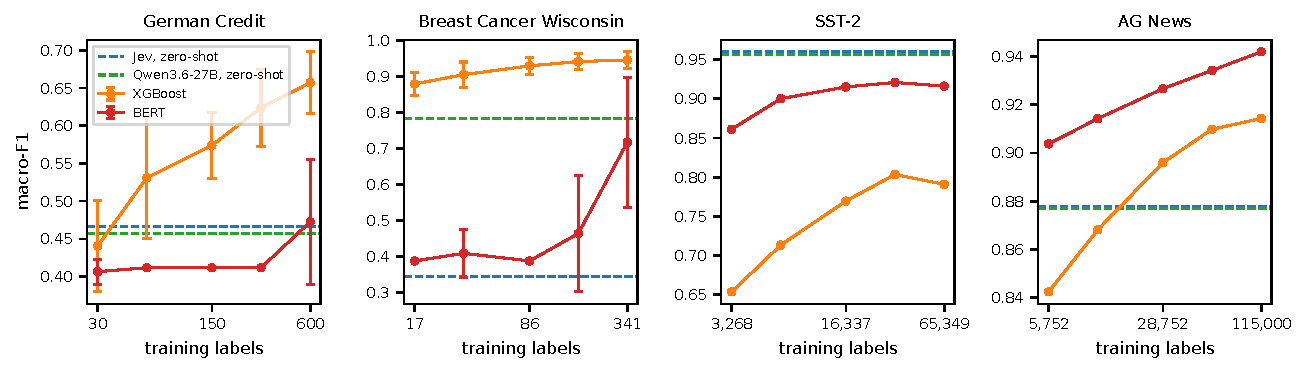
\includegraphics[width=\linewidth]{generated/figs/f1_by_labels}
  \caption{Macro-F1 on the evaluation examples against the number of training labels. Curves:
    supervised models. Dashed lines: zero-shot models, which use no training labels.}
  \label{fig:f1labels}
\end{figure}

\begin{table}[t]
  \caption{Labels, cost in USD and latency. Training cost is the whole recorded job, including
    model selection and the learning curve. Cost per 1,000 predictions: Jev, mean recorded
    request cost; Qwen, the billed scoring job allocated by scoring time, with inference time
    only in parentheses; XGBoost and BERT, measured batch inference time at list price. Latency:
    Jev, one API request; Qwen, one item sent alone, with batch throughput in parentheses;
    XGBoost and BERT, batch inference time per item.}
  \label{tab:costs}
  \centering\small
  \setlength{\tabcolsep}{4pt}
  \fittable{\begin{tabular}{llrcrll}
\toprule
Dataset & Model & Labels & Macro-F1 & Training & Per 1,000 & Latency \\
\midrule
\multirow{4}{*}{German Credit} & Jev & 0 & 0.467 & -- & 0.022 & 0.15\,s \\
 & Qwen3.6-27B & 0 & 0.457 & -- & 0.683 (0.642) & 0.95\,s (2.5/s) \\
 & XGBoost & 600 & 0.657 & 0.0097 & $<$0.0001 & 1.3\,$\mu$s \\
 & BERT & 600 & 0.473 & 0.148 & 0.0003 & 0.76\,ms \\
\addlinespace
\multirow{4}{*}{Breast Cancer Wisconsin} & Jev & 0 & 0.343 & -- & 0.030 & 0.14\,s \\
 & Qwen3.6-27B & 0 & 0.783 & -- & 1.34 (1.26) & 1.10\,s (1.3/s) \\
 & XGBoost & 341 & 0.945 & 0.010 & $<$0.0001 & 3.1\,$\mu$s \\
 & BERT & 341 & 0.716 & 0.129 & 0.0004 & 1.26\,ms \\
\addlinespace
\multirow{4}{*}{SST-2} & Jev & 0 & 0.960 & -- & 0.015 & 0.15\,s \\
 & Qwen3.6-27B & 0 & 0.956 & -- & 0.352 (0.331) & 0.92\,s (4.8/s) \\
 & XGBoost & 65{,}349 & 0.791 & 0.024 & $<$0.0001 & 0.01\,ms \\
 & BERT & 65{,}349 & 0.916 & 0.457 & $<$0.0001 & 0.19\,ms \\
\addlinespace
\multirow{4}{*}{AG News} & Jev & 0 & 0.878 & -- & 0.018 & 0.15\,s \\
 & Qwen3.6-27B & 0 & 0.877 & -- & 0.586 (0.551) & 0.93\,s (2.9/s) \\
 & XGBoost & 115{,}000 & 0.914 & 0.157 & $<$0.0001 & 0.06\,ms \\
 & BERT & 115{,}000 & 0.942 & 1.09 & 0.0001 & 0.31\,ms \\
\bottomrule
\end{tabular}
}
\end{table}

With enough labels a fine-tuned encoder overtakes both zero-shot models on topic classification:
BERT reaches macro-F1 \MacroFOneBertAgnews{} on AG News against \MacroFOneJevAgnews{} for Jev,
and first matches Jev at \LabelsToMatchJevBertAgnews{} training labels (XGBoost:
\LabelsToMatchJevXgbAgnews). On SST-2 neither supervised model matches the zero-shot ones at any
size tried: BERT reaches \MacroFOneBertSst{} with all \NTrainSst{} labels, against
\MacroFOneJevSst{} for Jev. On the tabular datasets XGBoost needs only its smallest training set
to exceed both zero-shot models.

A Jev prediction cost USD~\CostPerKJevSst{} to USD~\CostPerKJevWdbc{} per 1,000, depending on
prompt length, and took \JevLatencySst\,s. Self-hosting Qwen on \texttt{\QwenScoringInstance}
cost USD~\CostPerKQwenSst{} to USD~\CostPerKQwenWdbc{} per 1,000, which is \CostRatioQwenJevSst{}
to \CostRatioQwenJevWdbc{} times Jev's price, at \QwenLatencySst{} to \QwenLatencyWdbc\,s per
single item. The supervised models are cheaper per prediction by orders of magnitude once
trained; their cost is the training run (at most USD~\TrainUSDBertAgnews{} for BERT) and, above
all, the labels. Letting Qwen reason before answering raised its macro-F1 on every dataset on a
\ThinkSubsampleN-item sample (for example \ThinkSubFOneQwenWdbc{} to
\ThinkSubFOneQwenThinkWdbc{} on Breast Cancer Wisconsin) at many times the compute
(Table~\ref{tab:thinking}). Appendix~\ref{app:learning} gives the accuracy curves
(Figure~\ref{fig:learning}) and every point of both curves (Table~\ref{tab:learning}).

\section{Jev with Qwen in the loop}
\label{sec:escalation}

A class distribution also says when a second opinion is worth paying for. We keep Jev's
prediction when its maximum class probability is at least a threshold $t$ and take Qwen's
otherwise. The reported point uses the $t$ that maximizes macro-F1 on validation items only,
with ties broken towards fewer escalations; everything is computed from saved predictions
(Figure~\ref{fig:escalation}; Appendix~\ref{app:escalation} lists the validation items).

\begin{figure}[t]
  \centering
  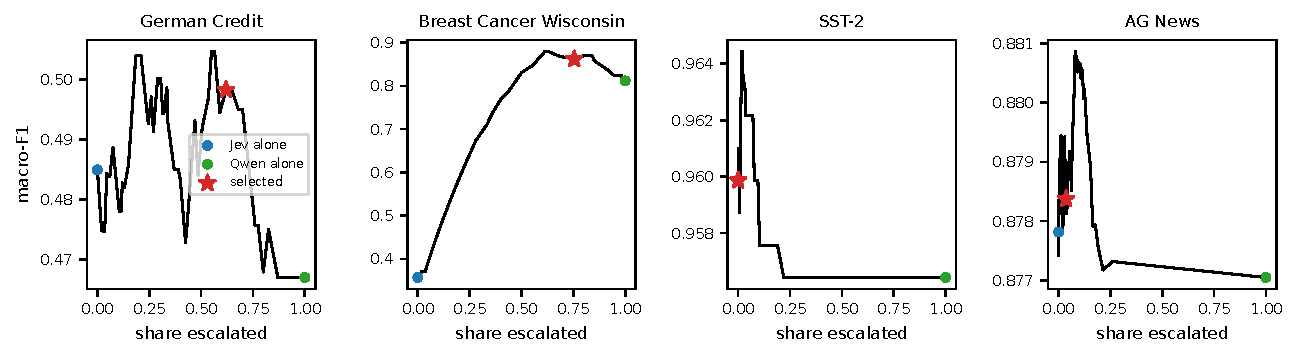
\includegraphics[width=\linewidth]{generated/figs/escalation}
  \caption{Macro-F1 of the ensemble against the share of evaluation items escalated to Qwen
    (first split repeat for the tabular datasets). The star marks the validation-selected
    threshold.}
  \label{fig:escalation}
\end{figure}

\begin{table}[t]
  \caption{Escalation of low-confidence Jev predictions to Qwen3.6-27B: macro-F1 of each model
    alone and of the ensemble at the validation-selected threshold $t$, the share of items
    escalated, the cost per 1,000 predictions, and the Jev errors at its highest reported
    confidence, which no threshold can reach without escalating every item at that confidence.}
  \label{tab:escalation}
  \centering\small
  \setlength{\tabcolsep}{4pt}
  \fittable{\begin{tabular}{lccccccr}
\toprule
Dataset & Jev & Qwen & $t$ & Share & Ensemble & USD/1,000 & Unreachable \\
\midrule
German Credit & 0.467\,{\scriptsize$\pm$0.019} & 0.457\,{\scriptsize$\pm$0.025} & 0.88 & 0.58 & 0.478\,{\scriptsize$\pm$0.029} & 0.421 & 5 of 103 \\
Breast Cancer Wisconsin & 0.343\,{\scriptsize$\pm$0.019} & 0.783\,{\scriptsize$\pm$0.029} & 0.85 & 0.69 & 0.856\,{\scriptsize$\pm$0.027} & 0.950 & 0 of 66 \\
SST-2 & 0.960 & 0.956 & 0.00 & 0.00 & 0.960 & 0.015 & 5 of 35 \\
AG News & 0.878 & 0.877 & 0.65 & 0.04 & 0.878 & 0.040 & 307 of 923 \\
\bottomrule
\end{tabular}
}
\end{table}

The outcome depends on what Jev's confidence knows (Table~\ref{tab:escalation}). On Breast Cancer
Wisconsin the ensemble beats both of its members: macro-F1 \EscFOneWdbc{} against
\EscJevFOneWdbc{} for Jev and \EscQwenFOneWdbc{} for Qwen, escalating \EscShareWdbc{} of the
items. Jev's confident predictions there are mostly right, and the ones it is unsure of are
better left to Qwen. On German Credit, where neither model ranks the rows, escalating
\EscShareGerman{} of them moves macro-F1 only from \EscJevFOneGerman{} to \EscFOneGerman. On
SST-2 the selected threshold escalates nothing. On AG News \EscShareAgnews{} of the items are
escalated and macro-F1 stays at \EscFOneAgnews: the two models are equally accurate, and
\EscUnreachableAgnews{} of Jev's \EscErrorsAgnews{} errors carry its highest reported confidence,
shared by \EscShareAtMaxAgnews{} of all items. Escalation is paid for at Qwen's price: USD
\EscCostPerKWdbc{} per 1,000 predictions on Breast Cancer Wisconsin against USD
\CostPerKJevWdbc{} for Jev alone.

\section{Threshold selection}
\label{sec:thresholding}

With class probabilities a decision can be tuned after the fact: predict the positive class when
$\mu_x(\{\text{positive}\}) \ge t$. We compare the default $t$, the analytic cost threshold
$C_{\text{FP}}/(C_{\text{FP}} + C_{\text{FN}})$, which is optimal under
calibration~\citep{elkan2001cost}, and the threshold that minimizes mean decision cost on
validation examples. German Credit has a canonical cost matrix (\CostRatioGerman); for Breast
Cancer Wisconsin we assume \CostRatioWdbc{} for a missed malignant case and for SST-2 symmetric
costs.

\begin{table}[t]
  \caption{Mean decision cost at the default and the analytic threshold, the validation-selected
    threshold $t$ with its cost, and accuracy before and after selection. Tabular values are
    means over \NRepeats{} split repeats. All models and all metrics are in
    Table~\ref{tab:thresholds-all}, and further sweeps in Figure~\ref{fig:threshold-more}.}
  \label{tab:thresholds}
  \centering\small
  \begin{tabular}{llcccccc}
\toprule
 & & \multicolumn{2}{c}{Cost at fixed $t$} & \multicolumn{2}{c}{Validation-selected} & \multicolumn{2}{c}{Accuracy} \\
\cmidrule(lr){3-4}\cmidrule(lr){5-6}\cmidrule(lr){7-8}
Dataset & Model & default & analytic & $t$ & cost & default & selected \\
\midrule
\multirow{2}{*}{German Credit} & Jev & 0.787 & 0.686 & 0.17 & 0.698 & 0.465 & 0.350 \\
 & XGBoost & 0.963 & 0.544 & 0.17 & 0.566 & 0.741 & 0.588 \\
\addlinespace
\multirow{2}{*}{Breast Cancer Wisconsin} & Jev & 0.605 & 0.630 & 0.77 & 0.395 & 0.405 & 0.735 \\
 & XGBoost & 0.170 & 0.124 & 0.27 & 0.147 & 0.949 & 0.937 \\
\addlinespace
\multirow{2}{*}{SST-2} & Jev & 0.040 & 0.040 & 0.36 & 0.033 & 0.960 & 0.967 \\
 & XGBoost & 0.209 & 0.209 & 0.55 & 0.205 & 0.791 & 0.795 \\
\bottomrule
\end{tabular}

\end{table}

\begin{figure}[t]
  \centering
  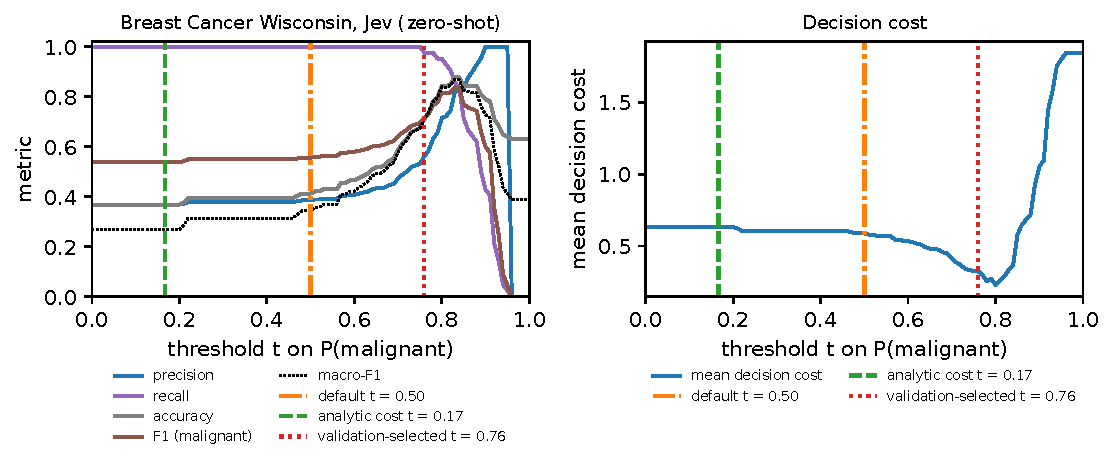
\includegraphics[width=0.86\linewidth]{generated/figs/threshold_wdbc_jev}
  \caption{Jev on Breast Cancer Wisconsin Diagnostic, first split repeat. Left: precision,
    recall, accuracy and positive-class F1 against the threshold $t$ (macro-F1 dashed). Right:
    mean decision cost against $t$. The three thresholds are marked in both panels.}
  \label{fig:threshold}
\end{figure}

Breast Cancer Wisconsin shows what the probabilities are worth when the default decision is not
(Table~\ref{tab:thresholds}, Figure~\ref{fig:threshold}). Jev's probability of \emph{malignant} ranks the rows well but sits
too high. The analytic threshold assumes calibration and moves the wrong way. The
validation-selected threshold moves to $t = \ThresholdValidationJevWdbc$: accuracy rises from
\ThrAccuracyDefaultJevWdbc{} to \ThrAccuracyValidationJevWdbc{} and the cost falls from
\ThrMeanCostDefaultJevWdbc{} to \ThrMeanCostValidationJevWdbc, using \ThrValLabelsJevWdbc{}
labels and no training. It does not close the gap to XGBoost (\ThrMeanCostValidationXgbWdbc).
On German Credit no threshold helps Jev much, because there is little ranking to exploit; for
the calibrated XGBoost the analytic threshold works as theory says, cutting its cost from
\ThrMeanCostDefaultXgbGerman{} to \ThrMeanCostAnalyticXgbGerman. On SST-2, where Jev is already
accurate and calibrated, selection changes little. A model that returns only a label is fixed at
one operating point; a distribution lets about a hundred labels place the decision.

\section{Estimating accuracy from few labels}
\label{sec:importance}

Labels are often the bottleneck for evaluating a deployed classifier. With class probabilities
the predicted uncertainty $u_i = 1 - p_{\max,i}$ can guide which items to label. We compare
uniform sampling with the confidence-guided proposal
$q_i = (1 - \varepsilon)\,u_i^{\alpha} / \sum_j u_j^{\alpha} + \varepsilon / N$ with
$\varepsilon = \ISEpsilon$ and $\alpha = \ISAlpha$~\citep{sawade2010are,kossen2021active},
estimating the error rate with the Hansen--Hurwitz estimator~\citep{hansen1943}, over
\ISTrials{} seeded trials per label budget; the sampler never sees a label it did not draw.

\begin{table}[t]
  \caption{RMSE of the accuracy estimate from $n$ labels, for uniform and confidence-guided
    sampling, and the ratio of their variances (uniform over guided; above 1 favours guided
    sampling), over \ISTrials{} trials.}
  \label{tab:importance}
  \centering\small
  \setlength{\tabcolsep}{4pt}
  \fittable{\begin{tabular}{lrrccccccccc}
\toprule
 & & & \multicolumn{3}{c}{$n = 25$} & \multicolumn{3}{c}{$n = 100$} & \multicolumn{3}{c}{$n = 400$} \\
\cmidrule(lr){4-6}\cmidrule(lr){7-9}\cmidrule(lr){10-12}
Dataset & Pool & Accuracy & uniform & guided & ratio & uniform & guided & ratio & uniform & guided & ratio \\
\midrule
German Credit & 1{,}000 & 0.471 & 0.097 & 0.212 & 0.21 & 0.049 & 0.105 & 0.22 & 0.025 & 0.052 & 0.23 \\
Breast Cancer Wisconsin & 569 & 0.427 & 0.101 & 0.090 & 1.27 & 0.048 & 0.045 & 1.14 & 0.024 & 0.021 & 1.32 \\
SST-2 & 872 & 0.960 & 0.039 & 0.057 & 0.46 & 0.020 & 0.029 & 0.47 & 0.010 & 0.014 & 0.48 \\
AG News & 7{,}600 & 0.879 & 0.067 & 0.135 & 0.24 & 0.032 & 0.069 & 0.22 & 0.017 & 0.032 & 0.28 \\
\bottomrule
\end{tabular}
}
\end{table}

The estimator is unbiased in practice (largest absolute bias \IsMaxAbsBias), but the guided
proposal reduces variance on only \IsDatasetsGuidedWins{} of the \NDatasets{} datasets
(Table~\ref{tab:importance}). At
\ISMaxBudget{} labels the ratio of uniform to guided variance is \IsVarRatioWdbcNFourZeroZero{}
on Breast Cancer Wisconsin and \IsVarRatioGermanNFourZeroZero, \IsVarRatioSstNFourZeroZero{} and
\IsVarRatioAgnewsNFourZeroZero{} on German Credit, SST-2 and AG News. The distribution itself
shows why. Jev rounds probabilities to two decimals, so \IsZeroUncertaintyAgnews{} of
\IsPoolAgnews{} AG News items have a reported uncertainty of exactly zero; they receive only the
minimum sampling probability yet contain \IsErrorsZeroUncertaintyAgnews{} of the
\IsErrorsAgnews{} errors, each weighted by $1/\varepsilon$. And for a 0/1 loss a proposal
proportional to the expected loss is not variance-optimal even under perfect calibration. The
check that reveals this needs only a small labelled sample (Appendix~\ref{app:importance},
Figure~\ref{fig:is}).

\section{Perturbation-based explanations}
\label{sec:explain}

Model-agnostic attribution needs only a real-valued function of the input, and with a class
distribution it is immediate: $f(z) = \mu_{x(z)}(\{c^\star\})$, Jev's probability of the class it
predicts on the full input when only the units in the coalition $z$ are kept (a feature line for
tabular rows, a word for text). We ran KernelSHAP~\citep{lundberg2017shap} and
LIME~\citep{ribeiro2016lime} on \ExExamplesGerman{} seeded examples per dataset, on live Jev, and
tested faithfulness by deleting the top-attributed units and re-querying.

\begin{table}[t]
  \caption{Explanations of Jev's predictions: mean drop in the predicted-class probability and
    share of label flips after deleting the top three attributed units, against three random
    units; Kendall's $\tau$ and top-3 overlap between KernelSHAP and LIME; and Jev requests used.}
  \label{tab:explain}
  \centering\small
  \setlength{\tabcolsep}{4pt}
  \fittable{\begin{tabular}{llrcccccccr}
\toprule
 & & & \multicolumn{3}{c}{Probability drop, $k=3$} & \multicolumn{2}{c}{Label flips, $k=3$} & \multicolumn{2}{c}{Agreement} & \\
\cmidrule(lr){4-6}\cmidrule(lr){7-8}\cmidrule(lr){9-10}
Dataset & Unit & Units & SHAP & LIME & random & SHAP & random & $\tau$ & top-3 & Jev requests \\
\midrule
German Credit & feature & 20 & 0.577 & 0.603 & 0.008 & 0.85 & 0.06 & 0.71 & 0.80 & 7{,}164 \\
Breast Cancer Wisconsin & feature & 30 & 0.065 & 0.155 & 0.010 & 0.05 & 0.02 & 0.37 & 0.35 & 7{,}969 \\
SST-2 & word & 18 & 0.401 & 0.419 & 0.096 & 0.40 & 0.09 & 0.51 & 0.70 & 6{,}666 \\
AG News & word & 34 & 0.075 & 0.091 & 0.003 & 0.10 & 0.00 & 0.19 & 0.27 & 7{,}919 \\
\bottomrule
\end{tabular}
}
\end{table}

Both methods run unmodified, and how useful they are depends on the dataset
(Table~\ref{tab:explain}). On German Credit
and SST-2 the explanations are faithful: deleting the three top KernelSHAP units lowers the
predicted-class probability by \ExDropShapGermanKThree{} and \ExDropShapSstKThree, against
\ExDropRandomGermanKThree{} and \ExDropRandomSstKThree{} for three random units. On Breast Cancer
Wisconsin and AG News they are weak (\ExDropShapWdbcKThree{} and \ExDropShapAgnewsKThree): with
\ExMeanUnitsWdbc{} correlated measurements, or \ExMeanUnitsAgnews{} words, no three units carry
the decision. The base value is informative in itself: with every feature removed, Jev still
gives \emph{bad} a probability of \ExEmptyInputPositiveGerman{} on German Credit, the bias that
Section~\ref{sec:metrics} measures. These explanations cost \ExRequestsTotal{} requests;
Appendix~\ref{app:explain} shows the deletion curves (Figure~\ref{fig:faithfulness}) and
example attributions (Figure~\ref{fig:attributions}).

\section{Limitations}
\label{sec:limitations}

The comparison is unequal by design: two models use no training labels and two use up to
\NTrainAgnews. Each dataset has one frozen template, never tuned; a public result on Breast
Cancer Wisconsin with a different serialization is much higher than ours, so our tabular numbers
describe this template, not Jev's best case. Qwen's distribution comes from scoring option names,
one of several ways to turn a generative model into a classifier, and carries numerical noise at
the second decimal; its cost and latency describe one deployment. No model is recalibrated. The
tabular datasets are small and their repeated splits overlap. Only German Credit has a canonical
cost matrix. Thinking was measured on \ThinkSubsampleN{} items per dataset, and explanations on
\ExExamplesGerman. All four datasets are widely circulated and the models may have seen them. A
fifth dataset was run and removed before writing; its costs are reported
(Appendix~\ref{app:protocol}).

\section{Conclusion}
\label{sec:conclusion}

A generative language model defines a measure on token strings; classes are reached only through
a parsing map that leaks probability, and the class distribution can only be estimated. A model
that returns a probability for every option defines the measure on $(C, 2^C)$ directly. On four
datasets that was enough to apply calibration analysis, threshold selection, escalation,
importance-sampled evaluation and perturbation-based explanations to Jev with standard tools,
and to score it with the same code as supervised classifiers; obtaining the same object from a
generative model took a scoring procedure of its own and far more computation per prediction.
What the toolbox found is mixed, and that is its value: accurate, usable probabilities on text;
a bias towards the adverse class on tables that a threshold or a second model repairs in one
case and not in the other; and guided sampling and escalation that pay off only where the
reported confidence is informative. The first thing the classical toolbox reports about a class
distribution is where it can be trusted.

\label{end:main}

\bibliographystyle{plainnat}
\bibliography{refs}

\clearpage
\appendix
\sloppy
\raggedbottom
\section{Prior public evaluations of Jev}
\label{app:prior}

Table~\ref{tab:prior} sets the public results next to ours. Every prior number in it was read from
its source on \PriorCheckedOn{} and is stored with the quoted text it came from; none was typed
into this paper. The protocols differ: each study uses its own template; the repository results
are for samples, with ECE over 10 bins; and the tabular benchmark uses a single
\PriorNStatsguysamWdbc-row split and a different serialization, which is the likely reason its
accuracy on Breast Cancer Wisconsin Diagnostic (\PriorAccStatsguysamWdbc) is far above ours
(\AccuracyJevWdbc).

\begin{table}[H]
  \caption{Prior public evaluations of zero-shot Jev on the datasets used here, next to our
    results at the default decision. Accuracy is at the argmax label.}
  \label{tab:prior}
  \centering\small
  \fittable{\begin{tabular}{llrrrrrr}
\toprule
 & & \multicolumn{3}{c}{Prior public evaluation} & \multicolumn{3}{c}{This paper (Jev, zero-shot)} \\
\cmidrule(lr){3-5}\cmidrule(lr){6-8}
Dataset & Source & $n$ & Acc. & ECE & $n$ & Acc. & ECE \\
\midrule
SST-2 & Deußer et al.~\citep{deusser2026jev} & 872 & 0.964 & 0.015 & 872 & 0.960 & 0.020 \\
AG News & Deußer et al.~\citep{deusser2026jev} & 7{,}600 & 0.885 & 0.077 & 7{,}600 & 0.879 & 0.082 \\
SST-2 & jevbench~\citep{jevbench2026} & 500 & 0.954 & 0.026 & 872 & 0.960 & 0.020 \\
AG News & jevbench~\citep{jevbench2026} & 500 & 0.843 & 0.112 & 7{,}600 & 0.879 & 0.082 \\
Breast Cancer Wisconsin Diagnostic & jev-classification-benchmark~\citep{statsguysam2026} & 114 & 0.842 & -- & 114 & 0.411 & 0.374 \\
German Credit & none found & -- & -- & -- & 200 & 0.467 & 0.364 \\
\bottomrule
\end{tabular}
}
\end{table}

\section{Protocol, label budgets and cost}
\label{app:protocol}

\paragraph{Models.}
Jev is queried through the \texttt{typesafe-sdk} Python client (version \SdkVersion) with one
\texttt{Choice} question per example; a missing tabular value is written as \texttt{unknown}, and
text is sent after collapsing whitespace. The text templates were tried once on
\TemplateCheckN{} training-split examples and frozen unchanged; the tabular templates were frozen
without being tried on data rows, because every row can be an evaluation row in some repeat.
XGBoost is trained with a fixed grid of \XgbGridSize{} configurations (tree depth and learning
rate), early stopping on the validation part (at most \XgbMaxRounds{} rounds, patience
\XgbPatience) and, for text, TF-IDF weights over unigrams and bigrams (at most \TfidfFeatures{}
features, \XgbTextBins{} histogram bins). BERT is \texttt{\BertModelId} (revision
\texttt{\BertRevision}); learning rates \BertLearningRates{} are each trained for up to
\BertMaxEpochs{} epochs (batch size \BertBatchSize) and the learning rate and epoch with the
lowest validation log-loss are kept, on the first split repeat for the tabular datasets. Inputs
are truncated at \BertMaxLengthGerman{} tokens (tabular), \BertMaxLengthAgnews{} (AG News) or
\BertMaxLengthSst{} (SST-2). Qwen is \texttt{\QwenModelId} (revision \texttt{\QwenRevision}) in
bf16. Its scores are computed with \texttt{transformers} \QwenTransformersVersion{} on
\texttt{\QwenScoringInstance}: the instruction and option list once per dataset, the rest of the
prompt once per item, and every option on a copy of that state, after a check on one item per
dataset that this equals a full recomputation. With thinking enabled the reasoning (greedy, at
most \ThinkMaxTokens{} tokens) is generated with vLLM~\citep{kwon2023vllm} \QwenVllmVersion{} and
the options are scored after it. All supervised training and all Qwen inference ran as managed
cloud training jobs (containers \texttt{sagemaker-xgboost:\XgbImageTag} and \breaktt{\BertImage}
for training).

\begin{table}[H]
  \caption{Labels used by each model, per split repeat. ``Early stopping, selection'' counts the
    validation labels used for early stopping and hyperparameter selection. Threshold selection
    applies to the binary datasets and reuses validation labels. The escalation threshold is
    selected on validation items predicted by both zero-shot models.}
  \label{tab:labels}
  \centering\small
  \fittable{\begin{tabular}{llrrrrr}
\toprule
Dataset & Model & Training & Early stopping, selection & Calibration & Threshold selection & Escalation threshold \\
\midrule
\multirow{4}{*}{German Credit} & Jev, zero-shot & 0 & 0 & 0 & 200 & 200 \\
 & Qwen3.6-27B, zero-shot & 0 & 0 & 0 & 200 & 200 \\
 & XGBoost, supervised & 600 & 200 & 0 & 200 & -- \\
 & BERT, supervised & 600 & 200 & 0 & 200 & -- \\
\addlinespace
\multirow{4}{*}{Breast Cancer Wisconsin} & Jev, zero-shot & 0 & 0 & 0 & 114 & 114 \\
 & Qwen3.6-27B, zero-shot & 0 & 0 & 0 & 114 & 114 \\
 & XGBoost, supervised & 341 & 114 & 0 & 114 & -- \\
 & BERT, supervised & 341 & 114 & 0 & 114 & -- \\
\addlinespace
\multirow{4}{*}{SST-2} & Jev, zero-shot & 0 & 0 & 0 & 500 & 500 \\
 & Qwen3.6-27B, zero-shot & 0 & 0 & 0 & 500 & 500 \\
 & XGBoost, supervised & 65{,}349 & 2{,}000 & 0 & 2{,}000 & -- \\
 & BERT, supervised & 65{,}349 & 2{,}000 & 0 & 2{,}000 & -- \\
\addlinespace
\multirow{4}{*}{AG News} & Jev, zero-shot & 0 & 0 & 0 & 0 & 500 \\
 & Qwen3.6-27B, zero-shot & 0 & 0 & 0 & 0 & 500 \\
 & XGBoost, supervised & 115{,}000 & 5{,}000 & 0 & 0 & -- \\
 & BERT, supervised & 115{,}000 & 5{,}000 & 0 & 0 & -- \\
\bottomrule
\end{tabular}
}
\end{table}

\paragraph{Budget and cost.}
The study was capped at \JevCap{} Jev inferences and used \JevInferencesUsed{}
(\JevRequestsPredict{} for predictions, \JevRequestsExplain{} for explanations,
\JevRequestsEscalationVal{} for escalation validation items, \JevRequestsTemplate{} for template
checks, \JevRequestsSmoke{} for connectivity checks). Every request is counted in a persistent
ledger before it is sent, and client retries are disabled; \JevFailedRequests{} requests failed.
Token counts exist for \JevRequestsWithTokens{} of the requests: \JevInputTokensM{} million input
tokens, USD~\JevCostUSD{} at USD~\JevPricePerMTok{} per million (Table~\ref{tab:cost}). All cloud
jobs together cost about USD~\AwsCostTotalUSD{} at list prices, under a limit of
USD~\AwsSpendLimit: USD~\AwsCostUSDXgb{} for XGBoost, USD~\AwsCostUSDBert{} for BERT
(\AwsGpuHoursBert{} GPU hours) and USD~\AwsCostUSDQwen{} for Qwen (\AwsGpuHoursQwen{} GPU hours),
counting stopped, failed and repeated executions. XGBoost was run a second time on every dataset
to record its inference time, and its predictions were \XgbRerunPredictions{} to the first ones.
Costs are computed from recorded token counts and from job records at list prices, not from
invoices.

\paragraph{A dataset that was run and removed.}
A fifth dataset, \RemovedDataset, was run and then removed from the study, because the
four-model comparison could not be completed on it within the compute limit. Everything spent on
it remains in the totals above: \RemovedJevRequests{} Jev requests (\RemovedJevTokensM{} million
input tokens, USD~\RemovedJevUSD), USD~\RemovedAwsDedicatedUSD{} of cloud jobs dedicated to it
(\RemovedAwsDedicatedExecutions{} executions), and a part of the USD~\RemovedAwsSharedUSD{} spent
on \RemovedAwsSharedExecutions{} exploratory Qwen executions that also covered other datasets and
cannot be split. No result for it is reported.

\paragraph{Societal impact.}
Two of the datasets stand for decisions that affect people: credit and medical diagnosis. Our
results are a caution for such uses. A zero-shot model's default decision was biased towards the
adverse class on both, on German Credit even with no evidence in the input, and nothing in its
text output would have revealed it. The positive side is that a class distribution makes the
bias measurable with standard tools and, where the ranking is sound, repairable with a small
labelled sample. The results describe four public benchmarks and one template per dataset and
should not be read as evidence that any of these models is fit or unfit for a deployment.

\paragraph{Uncertainty.}
For the held-out datasets we report 95\% bootstrap intervals (\BootstrapN{} resamples, fixed
seed). For the tabular datasets we report the mean and standard deviation over the \NRepeats{}
repeats; their test parts overlap across repeats, so the standard deviation describes split
variation, not an independent-sample standard error.

\begin{table}[H]
  \caption{Jev requests by stage. Input tokens are read from the logged responses and, for the
    \JevRequestsBeforeLoggingCached{} cached responses that predate the log, from the cache;
    \JevRequestsWithoutTokens{} request has no recorded token count. Output is not billed. The last
    row is the part of the total that was spent on the removed dataset.}
  \label{tab:cost}
  \centering\small
  \begin{tabular}{lrrrr}
\toprule
Stage & Requests & In request log & Input tokens (M) & Cost (USD) \\
\midrule
smoke & 3 & 2 & 0.00 & 0.000 \\
template & 60 & 60 & 0.06 & 0.003 \\
predict & 13{,}620 & 13{,}521 & 11.80 & 0.496 \\
explain & 35{,}317 & 35{,}317 & 25.81 & 1.084 \\
escalation\_val & 1{,}000 & 1{,}000 & 1.37 & 0.057 \\
\midrule
all stages & 50{,}000 & 49{,}900 & 39.04 & 1.640 \\
of which Banking77 (removed) & 9{,}198 & 9{,}198 & 21.10 & 0.886 \\
\bottomrule
\end{tabular}

\end{table}

\section{Full metrics and calibration}
\label{app:metrics}

\begin{table}[H]
  \caption{Classification metrics on identical evaluation examples. Brackets: 95\% bootstrap
    intervals (held-out datasets). $\pm$: standard deviation over \NRepeats{} split repeats
    (tabular datasets).}
  \label{tab:metrics}
  \centering\small
  \setlength{\tabcolsep}{4pt}
  \fittable{\begin{tabular}{llcccc}
\toprule
Dataset & Model & Accuracy & Macro-F1 & ROC-AUC & PR-AUC \\
\midrule
\multirow{4}{*}{German Credit} & Jev, zero-shot & 0.467\,{\scriptsize$\pm$0.019} & 0.467\,{\scriptsize$\pm$0.019} & 0.537\,{\scriptsize$\pm$0.030} & 0.316\,{\scriptsize$\pm$0.023} \\
 & Qwen3.6-27B, zero-shot & 0.544\,{\scriptsize$\pm$0.023} & 0.457\,{\scriptsize$\pm$0.025} & 0.496\,{\scriptsize$\pm$0.035} & 0.304\,{\scriptsize$\pm$0.028} \\
 & XGBoost, supervised & 0.741\,{\scriptsize$\pm$0.031} & 0.657\,{\scriptsize$\pm$0.041} & 0.768\,{\scriptsize$\pm$0.031} & 0.574\,{\scriptsize$\pm$0.046} \\
 & BERT, supervised & 0.705\,{\scriptsize$\pm$0.008} & 0.473\,{\scriptsize$\pm$0.083} & 0.683\,{\scriptsize$\pm$0.069} & 0.467\,{\scriptsize$\pm$0.071} \\
\addlinespace
\multirow{4}{*}{Breast Cancer Wisconsin} & Jev, zero-shot & 0.411\,{\scriptsize$\pm$0.014} & 0.343\,{\scriptsize$\pm$0.019} & 0.917\,{\scriptsize$\pm$0.021} & 0.878\,{\scriptsize$\pm$0.032} \\
 & Qwen3.6-27B, zero-shot & 0.825\,{\scriptsize$\pm$0.020} & 0.783\,{\scriptsize$\pm$0.029} & 0.969\,{\scriptsize$\pm$0.012} & 0.957\,{\scriptsize$\pm$0.012} \\
 & XGBoost, supervised & 0.949\,{\scriptsize$\pm$0.021} & 0.945\,{\scriptsize$\pm$0.023} & 0.985\,{\scriptsize$\pm$0.015} & 0.982\,{\scriptsize$\pm$0.015} \\
 & BERT, supervised & 0.778\,{\scriptsize$\pm$0.092} & 0.716\,{\scriptsize$\pm$0.182} & 0.853\,{\scriptsize$\pm$0.057} & 0.829\,{\scriptsize$\pm$0.044} \\
\addlinespace
\multirow{4}{*}{SST-2} & Jev, zero-shot & 0.960\,{\scriptsize[0.948,\,0.971]} & 0.960\,{\scriptsize[0.948,\,0.971]} & 0.987\,{\scriptsize[0.979,\,0.993]} & 0.986\,{\scriptsize[0.976,\,0.993]} \\
 & Qwen3.6-27B, zero-shot & 0.956\,{\scriptsize[0.943,\,0.968]} & 0.956\,{\scriptsize[0.943,\,0.968]} & 0.989\,{\scriptsize[0.984,\,0.994]} & 0.990\,{\scriptsize[0.984,\,0.995]} \\
 & XGBoost, supervised & 0.791\,{\scriptsize[0.763,\,0.819]} & 0.791\,{\scriptsize[0.762,\,0.818]} & 0.873\,{\scriptsize[0.848,\,0.896]} & 0.879\,{\scriptsize[0.849,\,0.905]} \\
 & BERT, supervised & 0.916\,{\scriptsize[0.896,\,0.935]} & 0.916\,{\scriptsize[0.896,\,0.935]} & 0.976\,{\scriptsize[0.968,\,0.983]} & 0.979\,{\scriptsize[0.971,\,0.986]} \\
\addlinespace
\multirow{4}{*}{AG News} & Jev, zero-shot & 0.879\,{\scriptsize[0.871,\,0.886]} & 0.878\,{\scriptsize[0.870,\,0.885]} & 0.961\,{\scriptsize[0.958,\,0.964]} & 0.901\,{\scriptsize[0.893,\,0.910]} \\
 & Qwen3.6-27B, zero-shot & 0.877\,{\scriptsize[0.870,\,0.885]} & 0.877\,{\scriptsize[0.870,\,0.884]} & 0.962\,{\scriptsize[0.958,\,0.965]} & 0.909\,{\scriptsize[0.900,\,0.917]} \\
 & XGBoost, supervised & 0.914\,{\scriptsize[0.908,\,0.921]} & 0.914\,{\scriptsize[0.908,\,0.921]} & 0.985\,{\scriptsize[0.983,\,0.986]} & 0.960\,{\scriptsize[0.955,\,0.965]} \\
 & BERT, supervised & 0.942\,{\scriptsize[0.936,\,0.947]} & 0.942\,{\scriptsize[0.937,\,0.947]} & 0.992\,{\scriptsize[0.991,\,0.993]} & 0.979\,{\scriptsize[0.976,\,0.982]} \\
\bottomrule
\end{tabular}
}
\end{table}

\begin{table}[H]
  \caption{Calibration: expected calibration error (\ECEBins{} equal-width bins), Brier score,
    log-loss, and mean confidence (mean of the maximum class probability). A reported probability
    of exactly zero for the true class is clipped at \LogLossClip{} in the log-loss.}
  \label{tab:calibration}
  \centering\small
  \setlength{\tabcolsep}{4pt}
  \fittable{\begin{tabular}{llcccc}
\toprule
Dataset & Model & ECE & Brier & Log-loss & Mean confidence \\
\midrule
\multirow{4}{*}{German Credit} & Jev, zero-shot & 0.364\,{\scriptsize$\pm$0.030} & 0.833\,{\scriptsize$\pm$0.041} & 2.136\,{\scriptsize$\pm$0.291} & 0.814 \\
 & Qwen3.6-27B, zero-shot & 0.136\,{\scriptsize$\pm$0.015} & 0.499\,{\scriptsize$\pm$0.017} & 0.694\,{\scriptsize$\pm$0.019} & 0.669 \\
 & XGBoost, supervised & 0.069\,{\scriptsize$\pm$0.017} & 0.346\,{\scriptsize$\pm$0.022} & 0.516\,{\scriptsize$\pm$0.027} & 0.757 \\
 & BERT, supervised & 0.060\,{\scriptsize$\pm$0.034} & 0.390\,{\scriptsize$\pm$0.024} & 0.574\,{\scriptsize$\pm$0.029} & 0.706 \\
\addlinespace
\multirow{4}{*}{Breast Cancer Wisconsin} & Jev, zero-shot & 0.374\,{\scriptsize$\pm$0.013} & 0.655\,{\scriptsize$\pm$0.014} & 0.865\,{\scriptsize$\pm$0.020} & 0.773 \\
 & Qwen3.6-27B, zero-shot & 0.072\,{\scriptsize$\pm$0.026} & 0.223\,{\scriptsize$\pm$0.012} & 0.341\,{\scriptsize$\pm$0.015} & 0.857 \\
 & XGBoost, supervised & 0.036\,{\scriptsize$\pm$0.010} & 0.074\,{\scriptsize$\pm$0.032} & 0.139\,{\scriptsize$\pm$0.064} & 0.966 \\
 & BERT, supervised & 0.115\,{\scriptsize$\pm$0.052} & 0.312\,{\scriptsize$\pm$0.062} & 0.486\,{\scriptsize$\pm$0.075} & 0.747 \\
\addlinespace
\multirow{4}{*}{SST-2} & Jev, zero-shot & 0.020\,{\scriptsize[0.014,\,0.034]} & 0.064\,{\scriptsize[0.047,\,0.082]} & 0.255\,{\scriptsize[0.138,\,0.397]} & 0.967 \\
 & Qwen3.6-27B, zero-shot & 0.023\,{\scriptsize[0.017,\,0.038]} & 0.073\,{\scriptsize[0.054,\,0.093]} & 0.159\,{\scriptsize[0.112,\,0.214]} & 0.974 \\
 & XGBoost, supervised & 0.026\,{\scriptsize[0.022,\,0.061]} & 0.290\,{\scriptsize[0.261,\,0.320]} & 0.451\,{\scriptsize[0.411,\,0.493]} & 0.799 \\
 & BERT, supervised & 0.054\,{\scriptsize[0.040,\,0.075]} & 0.138\,{\scriptsize[0.109,\,0.170]} & 0.259\,{\scriptsize[0.204,\,0.321]} & 0.966 \\
\addlinespace
\multirow{4}{*}{AG News} & Jev, zero-shot & 0.082\,{\scriptsize[0.076,\,0.090]} & 0.204\,{\scriptsize[0.192,\,0.216]} & 1.464\,{\scriptsize[1.337,\,1.591]} & 0.960 \\
 & Qwen3.6-27B, zero-shot & 0.099\,{\scriptsize[0.093,\,0.107]} & 0.219\,{\scriptsize[0.207,\,0.233]} & 0.925\,{\scriptsize[0.857,\,0.997]} & 0.976 \\
 & XGBoost, supervised & 0.032\,{\scriptsize[0.027,\,0.038]} & 0.135\,{\scriptsize[0.127,\,0.143]} & 0.270\,{\scriptsize[0.256,\,0.286]} & 0.887 \\
 & BERT, supervised & 0.018\,{\scriptsize[0.014,\,0.023]} & 0.091\,{\scriptsize[0.084,\,0.100]} & 0.179\,{\scriptsize[0.165,\,0.197]} & 0.958 \\
\bottomrule
\end{tabular}
}
\end{table}

\begin{figure}[H]
  \centering
  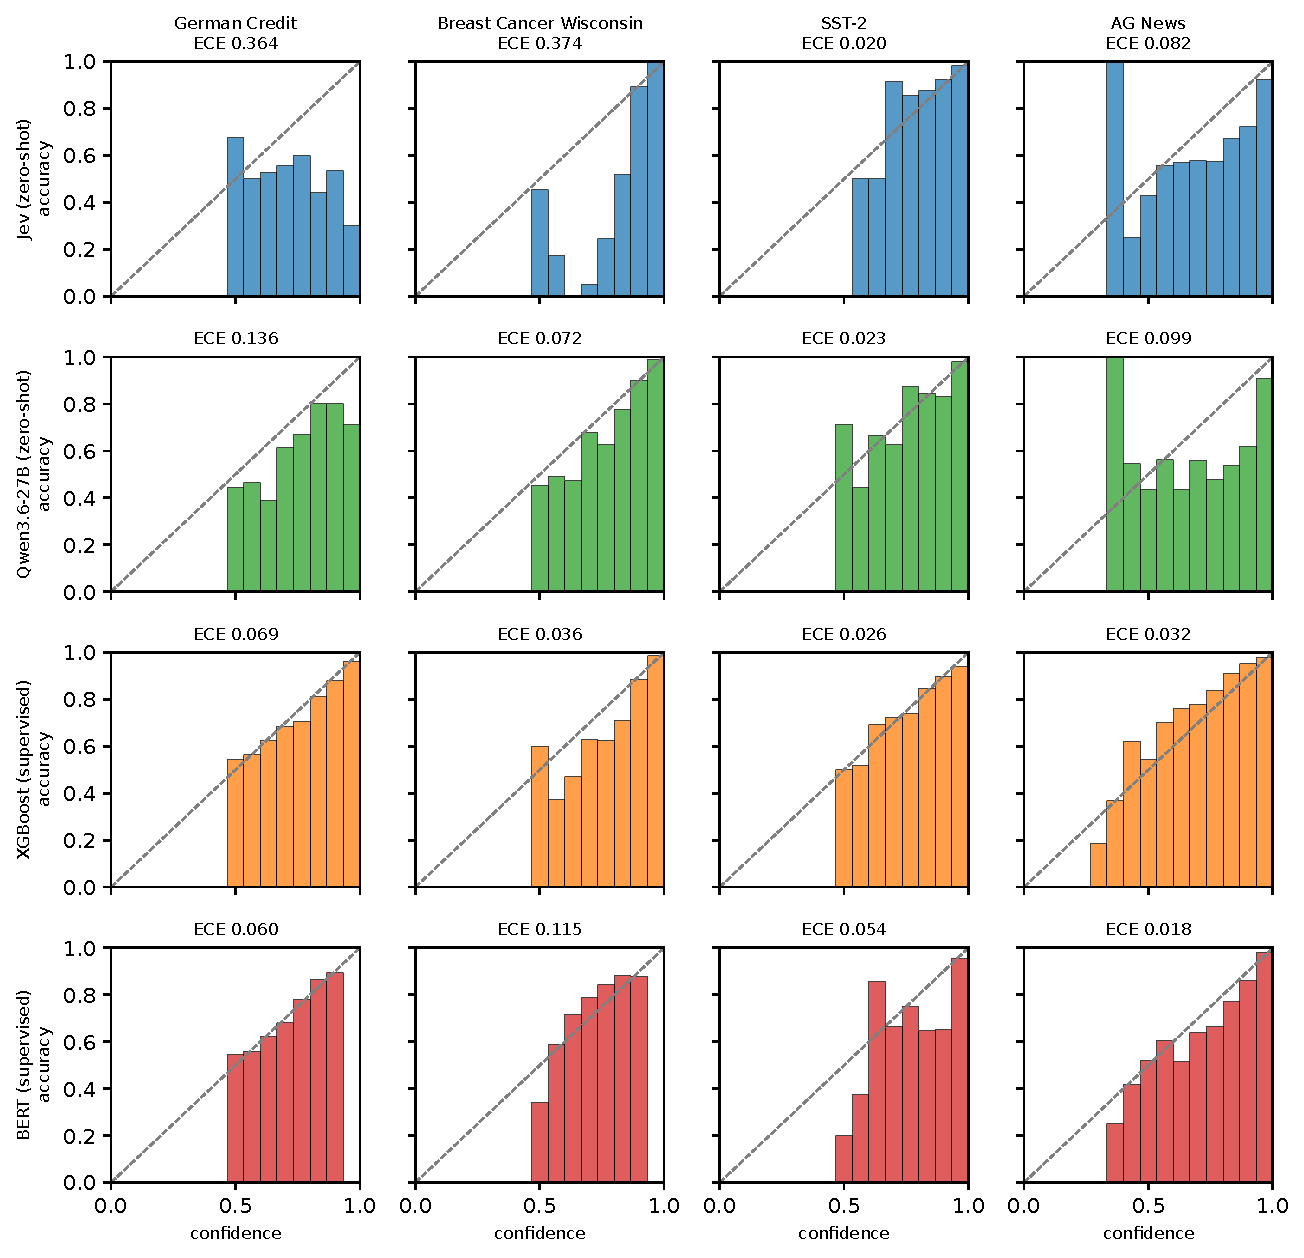
\includegraphics[width=\linewidth]{generated/figs/reliability}
  \caption{Reliability diagrams: accuracy against the maximum class probability, in \ECEBins{}
    equal-width bins. Rows, top to bottom: Jev and Qwen3.6-27B (zero-shot), XGBoost and BERT
    (supervised). Tabular datasets pool the test parts of all split repeats.}
  \label{fig:reliability}
\end{figure}

\section{Learning curves and thinking}
\label{app:learning}

On the text datasets, XGBoost sees only TF-IDF features and reaches 0.791 on SST-2 and 0.914 on AG News (zero-shot Jev: 0.960 and 0.879).
The learning curves (Figure~\ref{fig:learning}) put the comparison in terms of labels: on SST-2 it does not reach zero-shot Jev even with all 65{,}349 training labels; on AG News it first reaches zero-shot Jev at 28{,}752 training labels.


\begin{figure}[H]
  \centering
  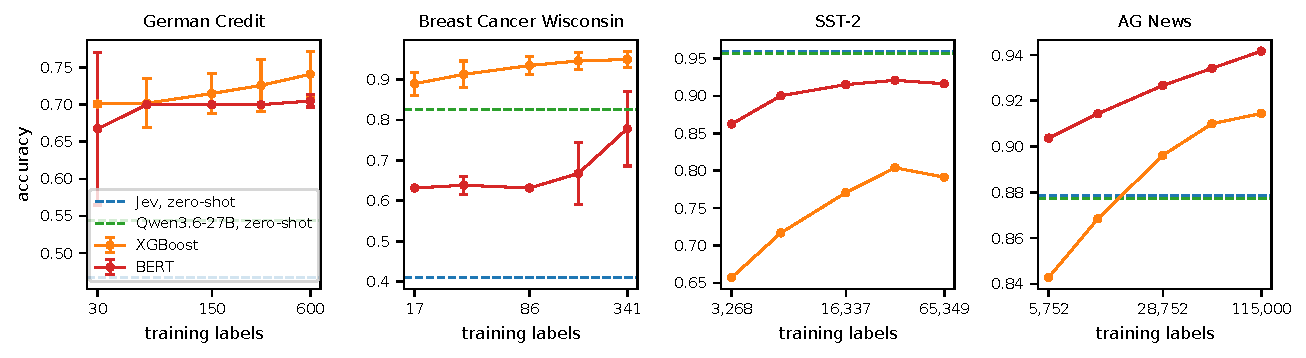
\includegraphics[width=\linewidth]{generated/figs/learning_curves}
  \caption{Accuracy of XGBoost and BERT on the evaluation examples against the number of
    training labels, with the zero-shot models as horizontal references.}
  \label{fig:learning}
\end{figure}

\begin{table}[H]
  \caption{XGBoost and BERT on the evaluation examples when trained on nested, stratified
    fractions of the training part with their selected configuration (mean over split repeats
    for the tabular datasets). The first row of each dataset gives the zero-shot models, at zero
    training labels, as accuracy / macro-F1.}
  \label{tab:learning}
  \centering\small
  \begin{tabular}{lrcccc}
\toprule
 & & \multicolumn{2}{c}{XGBoost, supervised} & \multicolumn{2}{c}{BERT, supervised} \\
\cmidrule(lr){3-4}\cmidrule(lr){5-6}
Dataset & Training labels & Accuracy & Macro-F1 & Accuracy & Macro-F1 \\
\midrule
\multirow{6}{*}{German Credit} & 0 & \multicolumn{4}{l}{Jev 0.467 / 0.467; Qwen3.6-27B 0.544 / 0.457} \\
 & 30 & 0.701 & 0.441 & 0.667 & 0.407 \\
 & 60 & 0.702 & 0.531 & 0.700 & 0.412 \\
 & 150 & 0.715 & 0.574 & 0.700 & 0.412 \\
 & 300 & 0.726 & 0.624 & 0.700 & 0.412 \\
 & 600 & 0.741 & 0.657 & 0.705 & 0.473 \\
\addlinespace
\multirow{6}{*}{Breast Cancer Wisconsin} & 0 & \multicolumn{4}{l}{Jev 0.411 / 0.343; Qwen3.6-27B 0.825 / 0.783} \\
 & 17 & 0.889 & 0.879 & 0.632 & 0.387 \\
 & 34 & 0.912 & 0.904 & 0.639 & 0.408 \\
 & 86 & 0.934 & 0.929 & 0.632 & 0.387 \\
 & 171 & 0.946 & 0.941 & 0.668 & 0.463 \\
 & 341 & 0.949 & 0.945 & 0.778 & 0.716 \\
\addlinespace
\multirow{6}{*}{SST-2} & 0 & \multicolumn{4}{l}{Jev 0.960 / 0.960; Qwen3.6-27B 0.956 / 0.956} \\
 & 3{,}268 & 0.657 & 0.654 & 0.862 & 0.861 \\
 & 6{,}535 & 0.717 & 0.713 & 0.900 & 0.900 \\
 & 16{,}337 & 0.771 & 0.769 & 0.915 & 0.915 \\
 & 32{,}674 & 0.804 & 0.804 & 0.921 & 0.921 \\
 & 65{,}349 & 0.791 & 0.791 & 0.916 & 0.916 \\
\addlinespace
\multirow{6}{*}{AG News} & 0 & \multicolumn{4}{l}{Jev 0.879 / 0.878; Qwen3.6-27B 0.877 / 0.877} \\
 & 5{,}752 & 0.843 & 0.842 & 0.904 & 0.904 \\
 & 11{,}500 & 0.868 & 0.868 & 0.914 & 0.914 \\
 & 28{,}752 & 0.896 & 0.896 & 0.927 & 0.927 \\
 & 57{,}500 & 0.910 & 0.910 & 0.934 & 0.934 \\
 & 115{,}000 & 0.914 & 0.914 & 0.942 & 0.942 \\
\bottomrule
\end{tabular}

\end{table}

\paragraph{Thinking.}
On the \ThinkSubsampleN{} items per dataset where Qwen also reasoned before answering, its
macro-F1 rose on every dataset: from \ThinkSubFOneQwenWdbc{} to \ThinkSubFOneQwenThinkWdbc{} on
Breast Cancer Wisconsin Diagnostic, \ThinkSubFOneQwenGerman{} to \ThinkSubFOneQwenThinkGerman{}
on German Credit, \ThinkSubFOneQwenSst{} to \ThinkSubFOneQwenThinkSst{} on SST-2 and
\ThinkSubFOneQwenAgnews{} to \ThinkSubFOneQwenThinkAgnews{} on AG News. These are small samples,
and the reasoning is long (\ThinkTokensWdbc{} tokens on average on Breast Cancer Wisconsin
Diagnostic, with \ThinkTruncatedGerman{} of German Credit items reaching the limit). Reasoning on
every item was projected at USD~\QwenThinkingAllProjectedUSD, which \QwenThinkingAllFits{} our
spending limit with a safety margin, so it was not run.

\begin{table}[H]
  \caption{Macro-F1 on the thinking subsample. Every model is scored on the same items.
    ``Thinking tokens'' is the mean length of the reasoning and ``Truncated'' the share of items
    whose reasoning reached the limit of \ThinkMaxTokens{} tokens.}
  \label{tab:thinking}
  \centering\small
  \fittable{\begin{tabular}{lrcccccrr}
\toprule
Dataset & $n$ & Jev & Qwen, off & Qwen, on & XGBoost & BERT & Thinking tokens & Truncated \\
\midrule
German Credit & 50 & 0.440 & 0.435 & 0.531 & 0.688 & 0.479 & 1{,}765 & 0.40 \\
Breast Cancer Wisconsin & 50 & 0.319 & 0.772 & 0.890 & 0.934 & 0.792 & 1{,}500 & 0.12 \\
SST-2 & 50 & 0.939 & 0.918 & 0.959 & 0.760 & 0.960 & 376 & 0.00 \\
AG News & 50 & 0.873 & 0.854 & 0.893 & 0.884 & 0.938 & 522 & 0.00 \\
\bottomrule
\end{tabular}
}
\end{table}

\section{Escalation: validation items}
\label{app:escalation}

The validation items for the escalation threshold are each repeat's validation part for the
tabular datasets, the \EscValLabelsSst{} threshold-selection items for SST-2, and
\EscValItemsNew{} seeded validation items for AG News that both models predicted for this
purpose.


\section{Threshold selection in full}
\label{app:thresholds}

Jev's threshold is selected on \ThrValLabelsJevGerman, \ThrValLabelsJevWdbc{} and
\ThrValLabelsJevSst{} validation labels for German Credit, Breast Cancer Wisconsin Diagnostic
and SST-2; on the tabular datasets this is repeated for each of the \NRepeats{} splits. On
Breast Cancer Wisconsin Diagnostic, at the default threshold Jev calls
\PredictedPositiveJevWdbc{} of the rows malignant, for a mean cost of
\ThrMeanCostDefaultJevWdbc; the analytic threshold (\ThresholdAnalyticJevWdbc) moves the wrong
way, to \ThrMeanCostAnalyticJevWdbc; the validation-selected threshold reaches
\ThrMeanCostValidationJevWdbc, with recall \ThrRecallValidationJevWdbc{} and precision
\ThrPrecisionValidationJevWdbc{} on malignant cases. On German Credit the cost is
\ThrMeanCostDefaultJevGerman{} at the default, \ThrMeanCostAnalyticJevGerman{} at the analytic and
\ThrMeanCostValidationJevGerman{} at the validation-selected threshold, and the lower cost is
bought by calling nearly every applicant bad (recall \ThrRecallValidationJevGerman, precision
\ThrPrecisionValidationJevGerman). On SST-2 the selected threshold
($t = \ThresholdValidationJevSst$) changes the cost only from \ThrMeanCostDefaultJevSst{} to
\ThrMeanCostValidationJevSst.


\begin{table}[H]
  \caption{Decisions at three thresholds on P(positive) for every model. Positive classes: bad
    (German Credit), malignant (Breast Cancer Wisconsin), positive (SST-2). Tabular values are
    means $\pm$ standard deviations over \NRepeats{} split repeats, and $t$ is the mean
    threshold. Costs: \CostRatioGerman{} (canonical), \CostRatioWdbc{} (illustrative),
    \CostRatioSst{} (illustrative).}
  \label{tab:thresholds-all}
  \centering\scriptsize
  \setlength{\tabcolsep}{3.5pt}
  \fittable{\begin{tabular}{lllcccccc}
\toprule
Dataset & Model & Threshold & $t$ & Precision & Recall & F1 (pos.) & Accuracy & Mean cost \\
\midrule
\multirow{12}{*}{German Credit} & \multirow{3}{*}{Jev, zero-shot} & default & 0.50 & 0.334\,{\scriptsize$\pm$0.012} & 0.790\,{\scriptsize$\pm$0.030} & 0.470\,{\scriptsize$\pm$0.016} & 0.465\,{\scriptsize$\pm$0.020} & 0.787\,{\scriptsize$\pm$0.048} \\
 &  & analytic & 0.17 & 0.313\,{\scriptsize$\pm$0.007} & 0.968\,{\scriptsize$\pm$0.018} & 0.473\,{\scriptsize$\pm$0.010} & 0.351\,{\scriptsize$\pm$0.016} & 0.686\,{\scriptsize$\pm$0.034} \\
 &  & validation-selected & 0.17 & 0.311\,{\scriptsize$\pm$0.008} & 0.960\,{\scriptsize$\pm$0.027} & 0.470\,{\scriptsize$\pm$0.011} & 0.350\,{\scriptsize$\pm$0.017} & 0.698\,{\scriptsize$\pm$0.042} \\
\cmidrule(lr){2-9}
 & \multirow{3}{*}{Qwen3.6-27B, zero-shot} & default & 0.50 & 0.244\,{\scriptsize$\pm$0.037} & 0.252\,{\scriptsize$\pm$0.043} & 0.248\,{\scriptsize$\pm$0.039} & 0.542\,{\scriptsize$\pm$0.023} & 1.356\,{\scriptsize$\pm$0.068} \\
 &  & analytic & 0.17 & 0.314\,{\scriptsize$\pm$0.009} & 0.955\,{\scriptsize$\pm$0.026} & 0.472\,{\scriptsize$\pm$0.012} & 0.360\,{\scriptsize$\pm$0.020} & 0.694\,{\scriptsize$\pm$0.043} \\
 &  & validation-selected & 0.14 & 0.306\,{\scriptsize$\pm$0.008} & 0.960\,{\scriptsize$\pm$0.039} & 0.464\,{\scriptsize$\pm$0.012} & 0.335\,{\scriptsize$\pm$0.024} & 0.713\,{\scriptsize$\pm$0.046} \\
\cmidrule(lr){2-9}
 & \multirow{3}{*}{XGBoost, supervised} & default & 0.50 & 0.604\,{\scriptsize$\pm$0.084} & 0.413\,{\scriptsize$\pm$0.071} & 0.488\,{\scriptsize$\pm$0.064} & 0.741\,{\scriptsize$\pm$0.031} & 0.963\,{\scriptsize$\pm$0.106} \\
 &  & analytic & 0.17 & 0.419\,{\scriptsize$\pm$0.017} & 0.883\,{\scriptsize$\pm$0.047} & 0.568\,{\scriptsize$\pm$0.021} & 0.597\,{\scriptsize$\pm$0.026} & 0.544\,{\scriptsize$\pm$0.062} \\
 &  & validation-selected & 0.17 & 0.415\,{\scriptsize$\pm$0.031} & 0.872\,{\scriptsize$\pm$0.091} & 0.560\,{\scriptsize$\pm$0.031} & 0.588\,{\scriptsize$\pm$0.057} & 0.566\,{\scriptsize$\pm$0.096} \\
\cmidrule(lr){2-9}
 & \multirow{3}{*}{BERT, supervised} & default & 0.50 & 0.231\,{\scriptsize$\pm$0.306} & 0.093\,{\scriptsize$\pm$0.137} & 0.125\,{\scriptsize$\pm$0.173} & 0.704\,{\scriptsize$\pm$0.007} & 1.384\,{\scriptsize$\pm$0.167} \\
 &  & analytic & 0.17 & 0.345\,{\scriptsize$\pm$0.051} & 0.930\,{\scriptsize$\pm$0.093} & 0.498\,{\scriptsize$\pm$0.038} & 0.426\,{\scriptsize$\pm$0.133} & 0.658\,{\scriptsize$\pm$0.048} \\
 &  & validation-selected & 0.21 & 0.352\,{\scriptsize$\pm$0.034} & 0.918\,{\scriptsize$\pm$0.085} & 0.506\,{\scriptsize$\pm$0.026} & 0.459\,{\scriptsize$\pm$0.085} & 0.639\,{\scriptsize$\pm$0.062} \\
\midrule
\multirow{12}{*}{Breast Cancer Wisconsin} & \multirow{3}{*}{Jev, zero-shot} & default & 0.50 & 0.382\,{\scriptsize$\pm$0.007} & 0.993\,{\scriptsize$\pm$0.012} & 0.552\,{\scriptsize$\pm$0.008} & 0.405\,{\scriptsize$\pm$0.014} & 0.605\,{\scriptsize$\pm$0.030} \\
 &  & analytic & 0.17 & 0.369\,{\scriptsize$\pm$0.001} & 1.000\,{\scriptsize$\pm$0.000} & 0.539\,{\scriptsize$\pm$0.001} & 0.370\,{\scriptsize$\pm$0.004} & 0.630\,{\scriptsize$\pm$0.004} \\
 &  & validation-selected & 0.77 & 0.605\,{\scriptsize$\pm$0.079} & 0.912\,{\scriptsize$\pm$0.083} & 0.721\,{\scriptsize$\pm$0.040} & 0.735\,{\scriptsize$\pm$0.068} & 0.395\,{\scriptsize$\pm$0.089} \\
\cmidrule(lr){2-9}
 & \multirow{3}{*}{Qwen3.6-27B, zero-shot} & default & 0.50 & 0.991\,{\scriptsize$\pm$0.019} & 0.531\,{\scriptsize$\pm$0.056} & 0.690\,{\scriptsize$\pm$0.048} & 0.825\,{\scriptsize$\pm$0.021} & 0.866\,{\scriptsize$\pm$0.104} \\
 &  & analytic & 0.17 & 0.838\,{\scriptsize$\pm$0.031} & 0.905\,{\scriptsize$\pm$0.032} & 0.870\,{\scriptsize$\pm$0.023} & 0.900\,{\scriptsize$\pm$0.018} & 0.240\,{\scriptsize$\pm$0.059} \\
 &  & validation-selected & 0.15 & 0.789\,{\scriptsize$\pm$0.058} & 0.926\,{\scriptsize$\pm$0.046} & 0.850\,{\scriptsize$\pm$0.027} & 0.878\,{\scriptsize$\pm$0.029} & 0.231\,{\scriptsize$\pm$0.059} \\
\cmidrule(lr){2-9}
 & \multirow{3}{*}{XGBoost, supervised} & default & 0.50 & 0.942\,{\scriptsize$\pm$0.023} & 0.919\,{\scriptsize$\pm$0.047} & 0.930\,{\scriptsize$\pm$0.030} & 0.949\,{\scriptsize$\pm$0.021} & 0.170\,{\scriptsize$\pm$0.088} \\
 &  & analytic & 0.17 & 0.879\,{\scriptsize$\pm$0.036} & 0.960\,{\scriptsize$\pm$0.046} & 0.917\,{\scriptsize$\pm$0.029} & 0.936\,{\scriptsize$\pm$0.022} & 0.124\,{\scriptsize$\pm$0.084} \\
 &  & validation-selected & 0.27 & 0.895\,{\scriptsize$\pm$0.042} & 0.943\,{\scriptsize$\pm$0.053} & 0.917\,{\scriptsize$\pm$0.026} & 0.937\,{\scriptsize$\pm$0.019} & 0.147\,{\scriptsize$\pm$0.089} \\
\cmidrule(lr){2-9}
 & \multirow{3}{*}{BERT, supervised} & default & 0.50 & 0.613\,{\scriptsize$\pm$0.333} & 0.593\,{\scriptsize$\pm$0.334} & 0.595\,{\scriptsize$\pm$0.321} & 0.778\,{\scriptsize$\pm$0.092} & 0.822\,{\scriptsize$\pm$0.574} \\
 &  & analytic & 0.17 & 0.560\,{\scriptsize$\pm$0.127} & 0.879\,{\scriptsize$\pm$0.080} & 0.671\,{\scriptsize$\pm$0.089} & 0.661\,{\scriptsize$\pm$0.161} & 0.518\,{\scriptsize$\pm$0.127} \\
 &  & validation-selected & 0.20 & 0.587\,{\scriptsize$\pm$0.103} & 0.845\,{\scriptsize$\pm$0.079} & 0.687\,{\scriptsize$\pm$0.079} & 0.709\,{\scriptsize$\pm$0.099} & 0.519\,{\scriptsize$\pm$0.168} \\
\midrule
\multirow{12}{*}{SST-2} & \multirow{3}{*}{Jev, zero-shot} & default & 0.50 & 0.979 & 0.941 & 0.960 & 0.960 & 0.040 \\
 &  & analytic & 0.50 & 0.979 & 0.941 & 0.960 & 0.960 & 0.040 \\
 &  & validation-selected & 0.36 & 0.975 & 0.959 & 0.967 & 0.967 & 0.033 \\
\cmidrule(lr){2-9}
 & \multirow{3}{*}{Qwen3.6-27B, zero-shot} & default & 0.50 & 0.981 & 0.932 & 0.956 & 0.956 & 0.044 \\
 &  & analytic & 0.50 & 0.981 & 0.932 & 0.956 & 0.956 & 0.044 \\
 &  & validation-selected & 0.29 & 0.972 & 0.953 & 0.962 & 0.962 & 0.038 \\
\cmidrule(lr){2-9}
 & \multirow{3}{*}{XGBoost, supervised} & default & 0.50 & 0.781 & 0.820 & 0.800 & 0.791 & 0.209 \\
 &  & analytic & 0.50 & 0.781 & 0.820 & 0.800 & 0.791 & 0.209 \\
 &  & validation-selected & 0.55 & 0.798 & 0.800 & 0.799 & 0.795 & 0.205 \\
\cmidrule(lr){2-9}
 & \multirow{3}{*}{BERT, supervised} & default & 0.50 & 0.901 & 0.939 & 0.920 & 0.916 & 0.084 \\
 &  & analytic & 0.50 & 0.901 & 0.939 & 0.920 & 0.916 & 0.084 \\
 &  & validation-selected & 0.49 & 0.901 & 0.939 & 0.920 & 0.916 & 0.084 \\
\bottomrule
\end{tabular}
}
\end{table}

\begin{figure}[H]
  \centering
  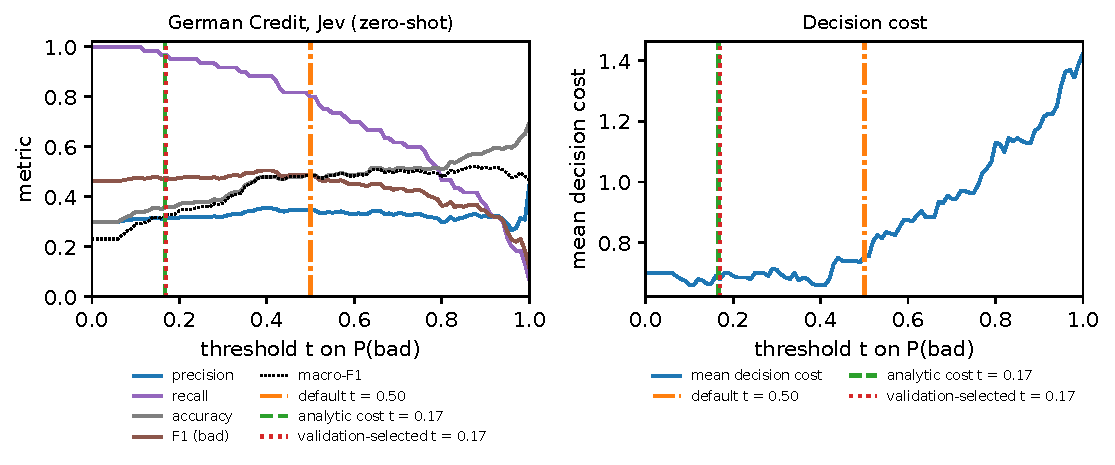
\includegraphics[width=0.8\linewidth]{generated/figs/threshold_german_jev}\\
  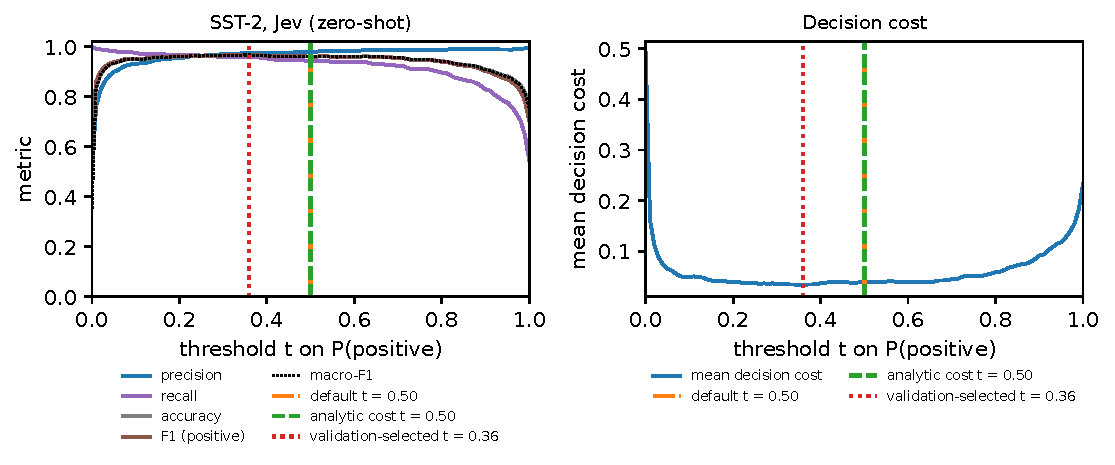
\includegraphics[width=0.8\linewidth]{generated/figs/threshold_sst2_jev}\\
  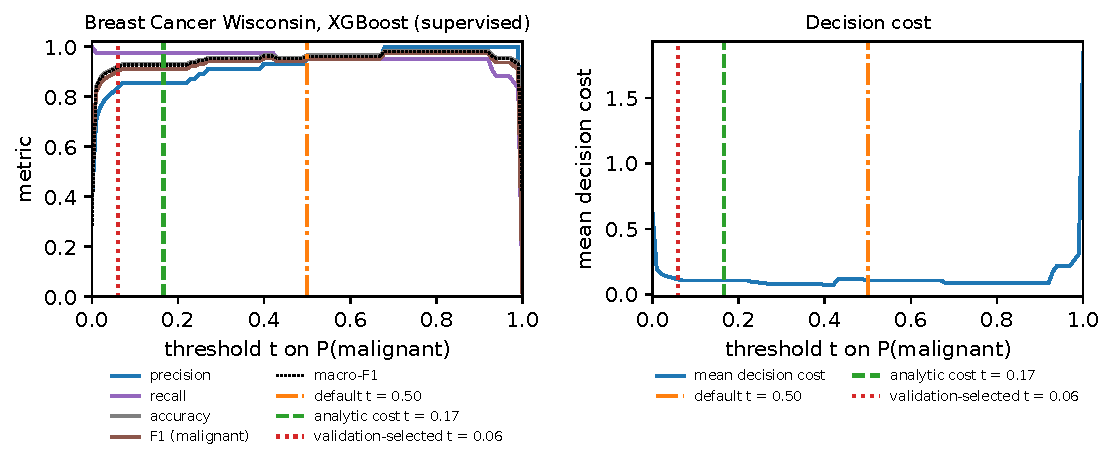
\includegraphics[width=0.8\linewidth]{generated/figs/threshold_wdbc_xgb}
  \caption{Threshold sweeps (first split repeat) for Jev on German Credit and SST-2, and for
    XGBoost on Breast Cancer Wisconsin Diagnostic. For SST-2 the costs are symmetric, so the
    analytic threshold coincides with the default.}
  \label{fig:threshold-more}
\end{figure}

\section{Importance sampling in full}
\label{app:importance}

For each dataset the pool is the fixed set of examples with cached Jev predictions. The sampling
procedure sees only those predictions: it draws $n$ items with replacement and asks for the
labels of the drawn items only. The Hansen--Hurwitz estimate of the error rate is
$\frac{1}{n}\sum_{j} \ell_{i_j}/(N q_{i_j})$, which is unbiased for any positive $q$, and accuracy
is one minus it. We run \ISTrials{} seeded trials at each budget $n \in \{\ISBudgets\}$ and
compare with the full-pool accuracy, which is used only as ground truth.


\begin{figure}[H]
  \centering
  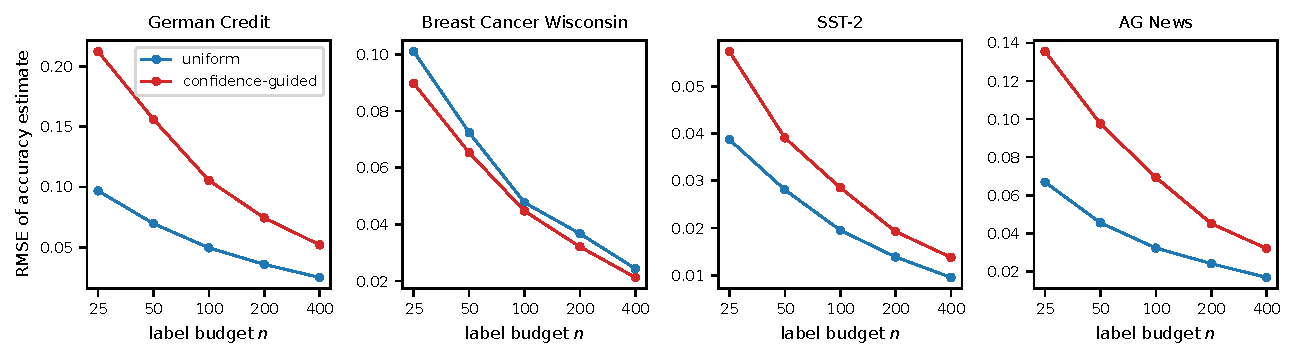
\includegraphics[width=\linewidth]{generated/figs/importance}
  \caption{RMSE of the accuracy estimate against the label budget.}
  \label{fig:is}
\end{figure}

Two things explain the result. First, because of the rounding, a large part of each text pool has
a reported uncertainty of exactly zero: \IsZeroUncertaintySst{} of \IsPoolSst{} items on SST-2
and \IsZeroUncertaintyAgnews{} of \IsPoolAgnews{} on AG News. Those items receive only the minimum
sampling probability $\varepsilon/N$, yet they contain \IsErrorsZeroUncertaintySst{} of the
\IsErrorsSst{} errors on SST-2 and \IsErrorsZeroUncertaintyAgnews{} of \IsErrorsAgnews{} on AG
News. Second, for a 0/1 loss a proposal proportional to the expected loss has the same variance
as uniform sampling under perfect calibration, and the optimum is proportional to the square
root of the expected loss. With $\alpha = \ISAlphaSqrt$ the ratios at $n = \ISMaxBudget$ are
\IsVarRatioHalfWdbc{} on Breast Cancer Wisconsin Diagnostic, \IsVarRatioHalfGerman{} on German
Credit, \IsVarRatioHalfSst{} on SST-2 and \IsVarRatioHalfAgnews{} on AG News: still below 1 on
\IsDatasetsSqrtBelowOne{} of the \NDatasets. Here the check says to sample uniformly unless the
reported uncertainties are first floored or recalibrated.

\section{Explanations in full}
\label{app:explain}

KernelSHAP uses \ShapCoalitions{} coalitions with the all-removed input as background, and LIME
\LimeSamples{} samples. Text examples were drawn among those with \ExMinWords{} to \ExMaxWords{}
words (\ExEligibleSst{} of \NTestSst{} for SST-2, \ExEligibleAgnews{} of \NTestAgnews{} for AG
News), so that deleting five words is meaningful. Faithfulness is tested by deleting the top-$k$
attributed units and re-querying Jev, against deleting $k$ random units (\ExRandomDraws{} draws).
KernelSHAP's attributions plus its base value reconstruct Jev's probability exactly (largest
additivity error \ExAdditivityMax). The two methods agree moderately to well on German Credit
and SST-2 ($\tau = \ExTauGerman$ and \ExTauSst) and little on Breast Cancer Wisconsin Diagnostic
and AG News ($\tau = \ExTauWdbc$ and \ExTauAgnews), where LIME's linear surrogate fits poorly
($R^2 = \ExLimeRTwoWdbc$ and \ExLimeRTwoAgnews, against \ExLimeRTwoGerman{} on German Credit).
With every feature removed, Jev assigns the positive class a probability of
\ExEmptyInputPositiveGerman{} on German Credit and \ExEmptyInputPositiveWdbc{} on Breast Cancer
Wisconsin Diagnostic, where the true shares are \TruePositiveGerman{} and \TruePositiveWdbc.
Perturbation methods are paid for in model calls: at most \ExRequestsPerExample{} per example
here, and \ExRequestsTotal{} requests in total (USD~\ExCostUSD), between \ExRequestsMin{} and
\ExRequestsMax{} per dataset after caching repeated inputs.


\begin{figure}[H]
  \centering
  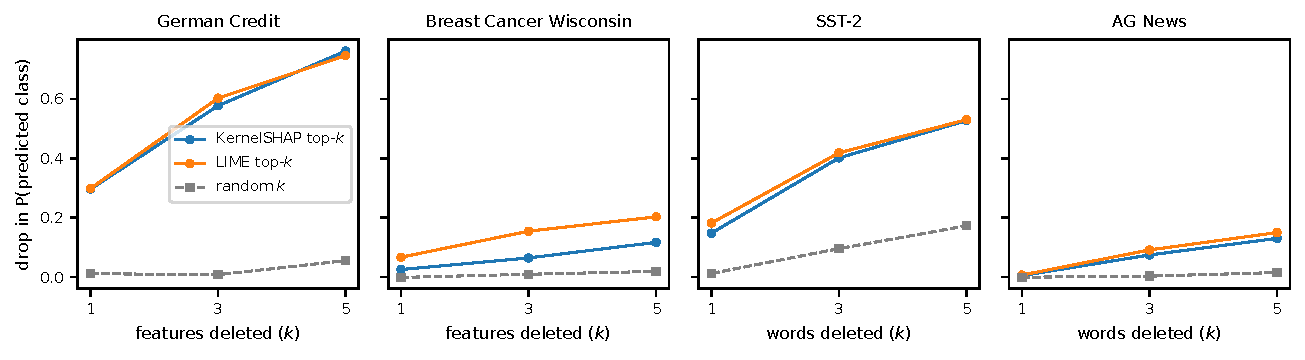
\includegraphics[width=\linewidth]{generated/figs/faithfulness}
  \caption{Deletion test: mean drop in Jev's predicted-class probability after deleting the $k$
    top-attributed units (KernelSHAP, LIME) or $k$ random units.}
  \label{fig:faithfulness}
\end{figure}

\begin{figure}[H]
  \centering
  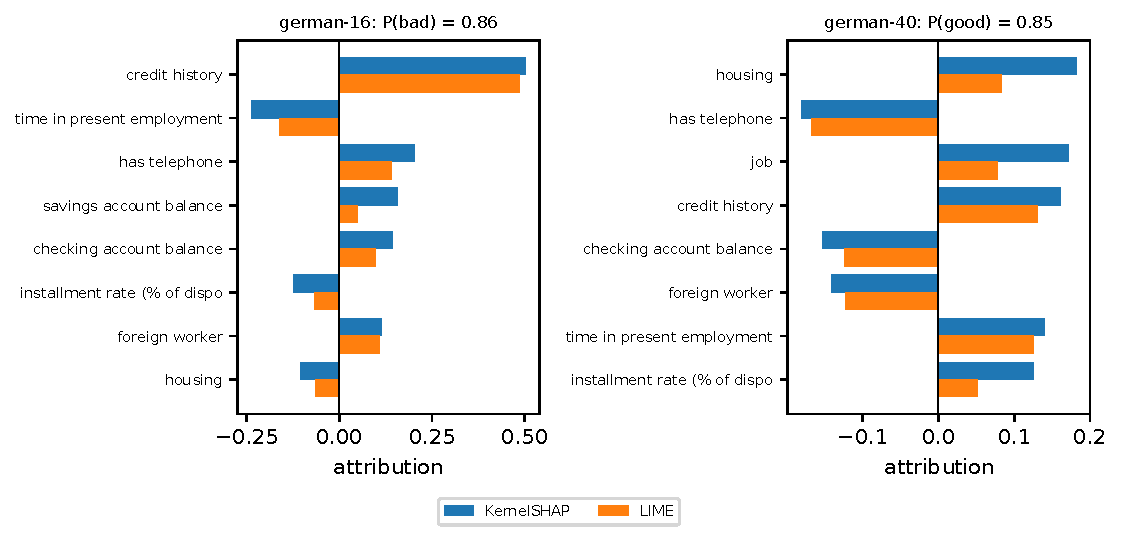
\includegraphics[width=0.49\linewidth]{generated/figs/attributions_german}\hfill
  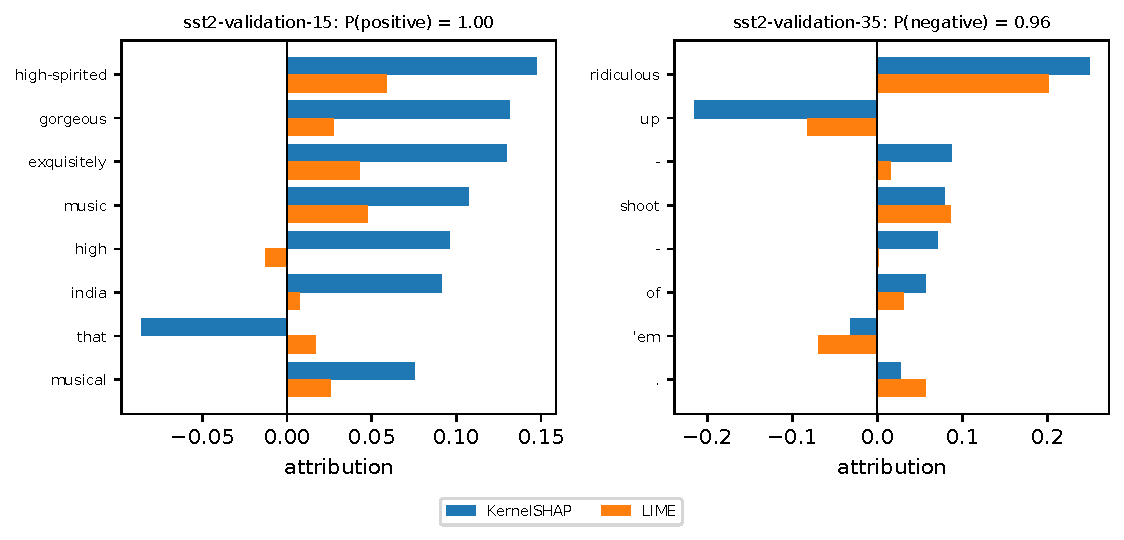
\includegraphics[width=0.49\linewidth]{generated/figs/attributions_sst2}
  \caption{KernelSHAP and LIME attributions for two German Credit applicants (left) and two
    SST-2 sentences (right): the eight units with the largest absolute KernelSHAP value.}
  \label{fig:attributions}
\end{figure}

\section{Exact requests and responses}
\label{app:payloads}

One complete exchange per dataset, copied from the request log. The example is the first
evaluation example, in a seeded order, whose request is in the log. The request and response
bodies are the JSON that crossed the wire, re-indented for reading; non-ASCII characters are shown
as JSON escapes. Headers are not recorded, so the API key cannot appear.

The \AuditUnlogged{} requests made before the log existed are not shown, because there is nothing
to copy. For \AuditUnloggedCached{} of them the response was cached in parsed form; regenerating
their requests from code and hashing them reproduces \AuditRegeneratedMatches{} of the
\AuditUnloggedCached{} stored cache keys, which shows that the same input, instructions, label
descriptions and model version were sent, but does not recover the payloads or the raw responses.
The remaining one was a connectivity check that was not cached.

\subsection*{German Credit}
Example \texttt{german-870}, gold label \texttt{good}; ledger number 951, sent 2026-09-30T13:\allowbreak{}43:\allowbreak{}22.039+00:\allowbreak{}00; \texttt{POST https://api.typesafe.ai/\allowbreak{}v1/\allowbreak{}systemone}; SDK \texttt{typesafe-sdk 0.7.2}; requested model \texttt{jev-1.13.0}, reported model \texttt{jev-1.13.0}; HTTP status 200; latency 0.18\,s.

\noindent\textbf{Request body as sent}
\begin{lstlisting}
{
 "state": "checking account balance: no checking account\nloan duration (months): 36\ncredit history: delayed previously\nloan purpose: furniture/equipment\ncredit amount (DM): 7678\nsavings account balance: 500 to 1000 DM\ntime in present employment: 4 to 7 years\ninstallment rate (% of disposable income): 2\npersonal status and sex: female div/dep/mar\nother debtors / guarantors: none\nyears at present residence: 4\nmost valuable property: car\nage (years): 40\nother installment plans: none\nhousing: own\nnumber of existing credits at this bank: 2\njob: skilled\nnumber of dependents: 1\nhas telephone: yes\nforeign worker: yes",
 "model": "jev-1.13.0",
 "questions": {
  "label": {
   "type": "choice",
   "instructions": "Assess the credit risk of a bank loan applicant described below. Fields that are not listed are unknown.",
   "criteria": {
    "good": "The applicant is a good credit risk and is likely to repay the loan.",
    "bad": "The applicant is a bad credit risk and is likely to default on the loan."
   }
  }
 }
}
\end{lstlisting}
\noindent\textbf{Response body as received}
\begin{lstlisting}
{
 "model": "jev-1.13.0",
 "answers": {
  "label": {
   "type": "choice",
   "choice": "good",
   "confidence": 0.13,
   "probabilities": {
    "good": 0.56,
    "bad": 0.44
   }
  }
 },
 "usage": {
  "input_tokens": 520,
  "output_tokens": 31
 }
}
\end{lstlisting}

\subsection*{Breast Cancer Wisconsin Diagnostic}
Example \texttt{wdbc-360}, gold label \texttt{benign}; ledger number 1423, sent 2026-09-30T13:\allowbreak{}43:\allowbreak{}34.432+00:\allowbreak{}00; \texttt{POST https://api.typesafe.ai/\allowbreak{}v1/\allowbreak{}systemone}; SDK \texttt{typesafe-sdk 0.7.2}; requested model \texttt{jev-1.13.0}, reported model \texttt{jev-1.13.0}; HTTP status 200; latency 0.11\,s.

\noindent\textbf{Request body as sent}
\begin{lstlisting}
{
 "state": "mean radius: 12.54\nmean texture: 18.07\nmean perimeter: 79.42\nmean area: 491.9\nmean smoothness: 0.07436\nmean compactness: 0.0265\nmean concavity: 0.001194\nmean concave points: 0.005449\nmean symmetry: 0.1528\nmean fractal dimension: 0.05185\nradius error: 0.3511\ntexture error: 0.9527\nperimeter error: 2.329\narea error: 28.3\nsmoothness error: 0.005783\ncompactness error: 0.004693\nconcavity error: 0.0007929\nconcave points error: 0.003617\nsymmetry error: 0.02043\nfractal dimension error: 0.001058\nworst radius: 13.72\nworst texture: 20.98\nworst perimeter: 86.82\nworst area: 585.7\nworst smoothness: 0.09293\nworst compactness: 0.04327\nworst concavity: 0.003581\nworst concave points: 0.01635\nworst symmetry: 0.2233\nworst fractal dimension: 0.05521",
 "model": "jev-1.13.0",
 "questions": {
  "label": {
   "type": "choice",
   "instructions": "Assess whether the breast mass described by the cell-nucleus measurements below is benign or malignant. Fields that are not listed are unknown.",
   "criteria": {
    "benign": "The mass is benign (not cancerous).",
    "malignant": "The mass is malignant (cancerous)."
   }
  }
 }
}
\end{lstlisting}
\noindent\textbf{Response body as received}
\begin{lstlisting}
{
 "model": "jev-1.13.0",
 "answers": {
  "label": {
   "type": "choice",
   "choice": "benign",
   "confidence": 0.06,
   "probabilities": {
    "malignant": 0.47,
    "benign": 0.53
   }
  }
 },
 "usage": {
  "input_tokens": 733,
  "output_tokens": 35
 }
}
\end{lstlisting}

\subsection*{SST-2}
Example \texttt{sst2-validation-36}, gold label \texttt{positive}; ledger number 1668, sent 2026-09-30T13:\allowbreak{}43:\allowbreak{}49.101+00:\allowbreak{}00; \texttt{POST https://api.typesafe.ai/\allowbreak{}v1/\allowbreak{}systemone}; SDK \texttt{typesafe-sdk 0.7.2}; requested model \texttt{jev-1.13.0}, reported model \texttt{jev-1.13.0}; HTTP status 200; latency 0.13\,s.

\noindent\textbf{Request body as sent}
\begin{lstlisting}
{
 "state": "the weight of the piece , the unerring professionalism of the chilly production , and the fascination embedded in the lurid topic prove recommendation enough .",
 "model": "jev-1.13.0",
 "questions": {
  "label": {
   "type": "choice",
   "instructions": "Classify the sentiment of the movie review sentence below.",
   "criteria": {
    "negative": "The sentence expresses a negative opinion of the movie.",
    "positive": "The sentence expresses a positive opinion of the movie."
   }
  }
 }
}
\end{lstlisting}
\noindent\textbf{Response body as received}
\begin{lstlisting}
{
 "model": "jev-1.13.0",
 "answers": {
  "label": {
   "type": "choice",
   "choice": "positive",
   "confidence": 0.96,
   "probabilities": {
    "negative": 0.02,
    "positive": 0.98
   }
  }
 },
 "usage": {
  "input_tokens": 359,
  "output_tokens": 31
 }
}
\end{lstlisting}

\subsection*{AG News}
Example \texttt{agnews-test-3752}, gold label \texttt{Business}; ledger number 9835, sent 2026-09-30T13:\allowbreak{}46:\allowbreak{}45.754+00:\allowbreak{}00; \texttt{POST https://api.typesafe.ai/\allowbreak{}v1/\allowbreak{}systemone}; SDK \texttt{typesafe-sdk 0.7.2}; requested model \texttt{jev-1.13.0}, reported model \texttt{jev-1.13.0}; HTTP status 200; latency 0.11\,s.

\noindent\textbf{Request body as sent}
\begin{lstlisting}
{
 "state": "McTeer: Lonesome Dove to be an Aggie NEW YORK (CNN/Money) - A New Economy champion, a lover of the Texas picker poets who write lovesick country songs...and, oh, by the way, a member of the Federal Reserve system for 36 years.",
 "model": "jev-1.13.0",
 "questions": {
  "label": {
   "type": "choice",
   "instructions": "Classify the topic of the news article below.",
   "criteria": {
    "World": "International news, politics, conflicts and world affairs.",
    "Sports": "Sports news: games, athletes, teams and competitions.",
    "Business": "Business and economic news: companies, markets, finance and the economy.",
    "Sci/Tech": "Science and technology news: computing, the internet, research, space and health science."
   }
  }
 }
}
\end{lstlisting}
\noindent\textbf{Response body as received}
\begin{lstlisting}
{
 "model": "jev-1.13.0",
 "answers": {
  "label": {
   "type": "choice",
   "choice": "Business",
   "confidence": 0.97,
   "probabilities": {
    "Sci/Tech": 0.0,
    "Business": 0.98,
    "Sports": 0.01,
    "World": 0.01
   }
  }
 },
 "usage": {
  "input_tokens": 446,
  "output_tokens": 47
 }
}
\end{lstlisting}


\section{Qwen prompts}
\label{app:qwen}

One prompt per dataset as rendered by Qwen's own tokenizer inside the job, with thinking
disabled, and the distribution obtained by scoring every option after it. The end-of-turn token
is part of every scored option, which makes an option that is a prefix of another a complete
answer.

\subsection*{German Credit}
Example \texttt{german-529}. Prompt with thinking disabled, as rendered by the model's tokenizer inside the job:
\begin{lstlisting}
<|im_start|>system
Assess the credit risk of a bank loan applicant described below. Fields that are not listed are unknown.

Options:
- good: The applicant is a good credit risk and is likely to repay the loan.
- bad: The applicant is a bad credit risk and is likely to default on the loan.

Answer with exactly one option name.<|im_end|>
<|im_start|>user
checking account balance: below 0 DM
loan duration (months): 6
credit history: existing paid
loan purpose: new car
credit amount (DM): 662
savings account balance: below 100 DM
time in present employment: less than 1 year
installment rate (% of disposable income): 3
personal status and sex: male single
other debtors / guarantors: none
years at present residence: 4
most valuable property: real estate
age (years): 41
other installment plans: none
housing: own
number of existing credits at this bank: 1
job: unskilled resident
number of dependents: 2
has telephone: yes
foreign worker: yes<|im_end|>
<|im_start|>assistant
<think>

</think>


\end{lstlisting}
Qwen3.6-27B's distribution: \texttt{good} 0.679, \texttt{bad} 0.321.

\subsection*{Breast Cancer Wisconsin Diagnostic}
Example \texttt{wdbc-477}. Prompt with thinking disabled, as rendered by the model's tokenizer inside the job:
\begin{lstlisting}
<|im_start|>system
Assess whether the breast mass described by the cell-nucleus measurements below is benign or malignant. Fields that are not listed are unknown.

Options:
- benign: The mass is benign (not cancerous).
- malignant: The mass is malignant (cancerous).

Answer with exactly one option name.<|im_end|>
<|im_start|>user
mean radius: 13.9
mean texture: 16.62
mean perimeter: 88.97
mean area: 599.4
mean smoothness: 0.06828
mean compactness: 0.05319
mean concavity: 0.02224
mean concave points: 0.01339
mean symmetry: 0.1813
mean fractal dimension: 0.05536
radius error: 0.1555
texture error: 0.5762
perimeter error: 1.392
area error: 14.03
smoothness error: 0.003308
compactness error: 0.01315
concavity error: 0.009904
concave points error: 0.004832
symmetry error: 0.01316
fractal dimension error: 0.002095
worst radius: 15.14
worst texture: 21.8
worst perimeter: 101.2
worst area: 718.9
worst smoothness: 0.09384
worst compactness: 0.2006
worst concavity: 0.1384
worst concave points: 0.06222
worst symmetry: 0.2679
worst fractal dimension: 0.07698<|im_end|>
<|im_start|>assistant
<think>

</think>


\end{lstlisting}
Qwen3.6-27B's distribution: \texttt{benign} 0.977, \texttt{malignant} 0.023.

\subsection*{SST-2}
Example \texttt{sst2-validation-2}. Prompt with thinking disabled, as rendered by the model's tokenizer inside the job:
\begin{lstlisting}
<|im_start|>system
Classify the sentiment of the movie review sentence below.

Options:
- negative: The sentence expresses a negative opinion of the movie.
- positive: The sentence expresses a positive opinion of the movie.

Answer with exactly one option name.<|im_end|>
<|im_start|>user
allows us to hope that nolan is poised to embark a major career as a commercial yet inventive filmmaker .<|im_end|>
<|im_start|>assistant
<think>

</think>


\end{lstlisting}
Qwen3.6-27B's distribution: \texttt{positive} 1.000, \texttt{negative} 0.000.

\subsection*{AG News}
Example \texttt{agnews-test-20}. Prompt with thinking disabled, as rendered by the model's tokenizer inside the job:
\begin{lstlisting}
<|im_start|>system
Classify the topic of the news article below.

Options:
- World: International news, politics, conflicts and world affairs.
- Sports: Sports news: games, athletes, teams and competitions.
- Business: Business and economic news: companies, markets, finance and the economy.
- Sci/Tech: Science and technology news: computing, the internet, research, space and health science.

Answer with exactly one option name.<|im_end|>
<|im_start|>user
IBM to hire even more new workers By the end of the year, the computing giant plans to have its biggest headcount since 1991.<|im_end|>
<|im_start|>assistant
<think>

</think>


\end{lstlisting}
Qwen3.6-27B's distribution: \texttt{Business} 0.997, \texttt{Sci/Tech} 0.001, \texttt{World} 0.001, \texttt{Sports} 0.001.


\section{Dataset documentation}
\label{app:datasets}

Evaluation identifiers were frozen on \FrozenAt{} (UTC), before any template check, training or
threshold selection; every stage verifies their hash before running.

\begin{table}[H]
  \caption{Datasets and split protocol. ``Jev requests'' is the number of examples Jev predicts:
    every row of the tabular datasets (each repeat's validation and test parts both use its
    predictions), and the held-out split of the text datasets plus, for SST-2, \NJevValSst{}
    validation items for threshold selection.}
  \label{tab:datasets-full}
  \centering\small
  \fittable{\begin{tabular}{llrllr}
\toprule
Dataset & Type & Classes & Evaluation examples & Train / validation & Jev requests \\
\midrule
German Credit & tabular & 2 & 10 stratified repeats, test 200 each & 600 / 200 per repeat & 1{,}000 \\
Breast Cancer Wisconsin Diagnostic & tabular & 2 & 10 stratified repeats, test 114 each & 341 / 114 per repeat & 569 \\
SST-2 & text & 2 & official validation split, 872 & 65{,}349 / 2{,}000 & 1{,}372 \\
AG News & text & 4 & official test split, 7{,}600 & 115{,}000 / 5{,}000 & 7{,}600 \\
\bottomrule
\end{tabular}
}
\end{table}

Table~\ref{tab:datasets-full} gives the split protocol in full.

\paragraph{German Credit.} \emph{Source:} OpenML dataset 31 (credit-g, version 1). \emph{Classes, in the order sent:} \texttt{good} (The applicant is a good credit risk and is likely to repay the loan., 621 evaluation examples); \texttt{bad} (The applicant is a bad credit risk and is likely to default on the loan., 264 evaluation examples). \emph{Positive class:} bad. \emph{Splits:} 10 stratified repeats with seeds 0--9; train 600, validation 200, test 200 in each; 885 distinct rows are a test row in some repeat. \emph{Input:} one \texttt{name: value} line per feature (20 features), categorical codes decoded; a missing value is written as \texttt{unknown} (0 missing values in this dataset). \emph{Instructions:} ``Assess the credit risk of a bank loan applicant described below. Fields that are not listed are unknown.''

\paragraph{Breast Cancer Wisconsin Diagnostic.} \emph{Source:} scikit-learn 1.9.1 sklearn.datasets.load\_breast\_cancer (UCI Machine Learning Repository, Breast Cancer Wisconsin (Diagnostic), 569 rows, 30 features). \emph{Classes, in the order sent:} \texttt{benign} (The mass is benign (not cancerous)., 317 evaluation examples); \texttt{malignant} (The mass is malignant (cancerous)., 189 evaluation examples). \emph{Positive class:} malignant. \emph{Splits:} 10 stratified repeats with seeds 0--9; train 341, validation 114, test 114 in each; 506 distinct rows are a test row in some repeat. \emph{Input:} one \texttt{name: value} line per feature (30 features), categorical codes decoded; a missing value is written as \texttt{unknown} (0 missing values in this dataset). \emph{Instructions:} ``Assess whether the breast mass described by the cell-nucleus measurements below is benign or malignant. Fields that are not listed are unknown.''

\paragraph{SST-2.} \emph{Source:} Hugging Face nyu-mll/\allowbreak{}glue, configuration sst2, revision bcdcba79\allowbreak{}d07bc864\allowbreak{}c1c254cc\allowbreak{}fcedcce5\allowbreak{}5bcc9a8c. \emph{Classes, in the order sent:} \texttt{negative} (The sentence expresses a negative opinion of the movie., 428 evaluation examples); \texttt{positive} (The sentence expresses a positive opinion of the movie., 444 evaluation examples). \emph{Positive class:} positive. \emph{Splits:} official validation split (872 examples, all used); validation 2{,}000 drawn stratified from the official training split with seed 0; training 65{,}349. \emph{Input:} the text itself, with whitespace runs collapsed to one space; leading and trailing space removed; no example is empty. \emph{Instructions:} ``Classify the sentiment of the movie review sentence below.''

\paragraph{AG News.} \emph{Source:} Hugging Face fancyzhx/\allowbreak{}ag\_news, revision eb185aad\allowbreak{}e064a813\allowbreak{}bc0b7f42\allowbreak{}de025955\allowbreak{}23103ca4. \emph{Classes, in the order sent:} \texttt{World} (International news, politics, conflicts and world affairs., 1900 evaluation examples); \texttt{Sports} (Sports news: games, athletes, teams and competitions., 1900 evaluation examples); \texttt{Business} (Business and economic news: companies, markets, finance and the economy., 1900 evaluation examples); \texttt{Sci/Tech} (Science and technology news: computing, the internet, research, space and health science., 1900 evaluation examples). \emph{Positive class:} not applicable. \emph{Splits:} official test split (7{,}600 examples, all used); validation 5{,}000 drawn stratified from the official training split with seed 0; training 115{,}000. \emph{Input:} the text itself, with whitespace runs collapsed to one space; leading and trailing space removed; no example is empty. \emph{Instructions:} ``Classify the topic of the news article below.''


\section{Per-class metrics}
\label{app:perclass}

\begin{table}[H]
\centering\scriptsize
\setlength{\tabcolsep}{3pt}
\fittable{\begin{tabular}{lrcccccccccccc}
\toprule
 & & \multicolumn{3}{c}{Jev} & \multicolumn{3}{c}{Qwen3.6-27B} & \multicolumn{3}{c}{XGBoost} & \multicolumn{3}{c}{BERT} \\
\cmidrule(lr){3-5}\cmidrule(lr){6-8}\cmidrule(lr){9-11}\cmidrule(lr){12-14}
Class & Support & P & R & F1 & P & R & F1 & P & R & F1 & P & R & F1 \\
\midrule
good & 1400 & 0.78 & 0.33 & 0.46 & 0.67 & 0.67 & 0.67 & 0.78 & 0.88 & 0.83 & 0.71 & 0.97 & 0.82 \\
bad & 600 & 0.33 & 0.79 & 0.47 & 0.24 & 0.24 & 0.24 & 0.60 & 0.41 & 0.49 & 0.55 & 0.09 & 0.16 \\
\bottomrule
\end{tabular}}
\caption{Per-class precision (P), recall (R) and F1 on German Credit. Support and metrics are pooled over the split repeats.}
\end{table}

\begin{table}[H]
\centering\scriptsize
\setlength{\tabcolsep}{3pt}
\fittable{\begin{tabular}{lrcccccccccccc}
\toprule
 & & \multicolumn{3}{c}{Jev} & \multicolumn{3}{c}{Qwen3.6-27B} & \multicolumn{3}{c}{XGBoost} & \multicolumn{3}{c}{BERT} \\
\cmidrule(lr){3-5}\cmidrule(lr){6-8}\cmidrule(lr){9-11}\cmidrule(lr){12-14}
Class & Support & P & R & F1 & P & R & F1 & P & R & F1 & P & R & F1 \\
\midrule
benign & 720 & 0.94 & 0.07 & 0.13 & 0.78 & 1.00 & 0.88 & 0.95 & 0.97 & 0.96 & 0.79 & 0.89 & 0.83 \\
malignant & 420 & 0.38 & 0.99 & 0.55 & 0.99 & 0.53 & 0.69 & 0.94 & 0.92 & 0.93 & 0.75 & 0.59 & 0.66 \\
\bottomrule
\end{tabular}}
\caption{Per-class precision (P), recall (R) and F1 on Breast Cancer Wisconsin Diagnostic. Support and metrics are pooled over the split repeats.}
\end{table}

\begin{table}[H]
\centering\scriptsize
\setlength{\tabcolsep}{3pt}
\fittable{\begin{tabular}{lrcccccccccccc}
\toprule
 & & \multicolumn{3}{c}{Jev} & \multicolumn{3}{c}{Qwen3.6-27B} & \multicolumn{3}{c}{XGBoost} & \multicolumn{3}{c}{BERT} \\
\cmidrule(lr){3-5}\cmidrule(lr){6-8}\cmidrule(lr){9-11}\cmidrule(lr){12-14}
Class & Support & P & R & F1 & P & R & F1 & P & R & F1 & P & R & F1 \\
\midrule
negative & 428 & 0.94 & 0.98 & 0.96 & 0.93 & 0.98 & 0.96 & 0.80 & 0.76 & 0.78 & 0.93 & 0.89 & 0.91 \\
positive & 444 & 0.98 & 0.94 & 0.96 & 0.98 & 0.93 & 0.96 & 0.78 & 0.82 & 0.80 & 0.90 & 0.94 & 0.92 \\
\bottomrule
\end{tabular}}
\caption{Per-class precision (P), recall (R) and F1 on SST-2.}
\end{table}

\begin{table}[H]
\centering\scriptsize
\setlength{\tabcolsep}{3pt}
\fittable{\begin{tabular}{lrcccccccccccc}
\toprule
 & & \multicolumn{3}{c}{Jev} & \multicolumn{3}{c}{Qwen3.6-27B} & \multicolumn{3}{c}{XGBoost} & \multicolumn{3}{c}{BERT} \\
\cmidrule(lr){3-5}\cmidrule(lr){6-8}\cmidrule(lr){9-11}\cmidrule(lr){12-14}
Class & Support & P & R & F1 & P & R & F1 & P & R & F1 & P & R & F1 \\
\midrule
World & 1900 & 0.90 & 0.89 & 0.90 & 0.92 & 0.87 & 0.90 & 0.93 & 0.91 & 0.92 & 0.97 & 0.93 & 0.95 \\
Sports & 1900 & 0.97 & 0.98 & 0.97 & 0.96 & 0.99 & 0.97 & 0.95 & 0.98 & 0.96 & 0.99 & 0.99 & 0.99 \\
Business & 1900 & 0.76 & 0.92 & 0.83 & 0.75 & 0.92 & 0.83 & 0.89 & 0.88 & 0.88 & 0.91 & 0.92 & 0.91 \\
Sci/Tech & 1900 & 0.92 & 0.72 & 0.81 & 0.90 & 0.74 & 0.81 & 0.89 & 0.89 & 0.89 & 0.90 & 0.93 & 0.92 \\
\bottomrule
\end{tabular}}
\caption{Per-class precision (P), recall (R) and F1 on AG News.}
\end{table}



% The NeurIPS paper checklist (sections/checklist.tex) was removed from this version at the
% author's request on 2026-10-02; a NeurIPS submission needs it back:
% \clearpage
% \section*{NeurIPS Paper Checklist}




\begin{enumerate}

\item {\bf Claims}
    \item[] Question: Do the main claims made in the abstract and introduction accurately reflect the paper's contributions and scope?
    \item[] Answer: \answerYes{}
    \item[] Justification: The abstract and introduction state the framing, the four-dataset evaluation of four models and the mixed findings; Sections~\ref{sec:metrics}--\ref{sec:explain} support each claim with generated numbers, and the introduction says the paper is not a leaderboard.
    \item[] Guidelines:
    \begin{itemize}
        \item The answer \answerNA{} means that the abstract and introduction do not include the claims made in the paper.
        \item The abstract and/or introduction should clearly state the claims made, including the contributions made in the paper and important assumptions and limitations. A \answerNo{} or \answerNA{} answer to this question will not be perceived well by the reviewers. 
        \item The claims made should match theoretical and experimental results, and reflect how much the results can be expected to generalize to other settings. 
        \item It is fine to include aspirational goals as motivation as long as it is clear that these goals are not attained by the paper. 
    \end{itemize}

\item {\bf Limitations}
    \item[] Question: Does the paper discuss the limitations of the work performed by the authors?
    \item[] Answer: \answerYes{}
    \item[] Justification: Section~\ref{sec:limitations} lists the unequal label budgets, the single untuned template per dataset, the scoring noise and single deployment of Qwen, the lack of recalibration, the small tabular datasets, the assumed cost matrices and the possibility that the models have seen the datasets.
    \item[] Guidelines:
    \begin{itemize}
        \item The answer \answerNA{} means that the paper has no limitation while the answer \answerNo{} means that the paper has limitations, but those are not discussed in the paper. 
        \item The authors are encouraged to create a separate ``Limitations'' section in their paper.
        \item The paper should point out any strong assumptions and how robust the results are to violations of these assumptions (e.g., independence assumptions, noiseless settings, model well-specification, asymptotic approximations only holding locally). The authors should reflect on how these assumptions might be violated in practice and what the implications would be.
        \item The authors should reflect on the scope of the claims made, e.g., if the approach was only tested on a few datasets or with a few runs. In general, empirical results often depend on implicit assumptions, which should be articulated.
        \item The authors should reflect on the factors that influence the performance of the approach. For example, a facial recognition algorithm may perform poorly when image resolution is low or images are taken in low lighting. Or a speech-to-text system might not be used reliably to provide closed captions for online lectures because it fails to handle technical jargon.
        \item The authors should discuss the computational efficiency of the proposed algorithms and how they scale with dataset size.
        \item If applicable, the authors should discuss possible limitations of their approach to address problems of privacy and fairness.
        \item While the authors might fear that complete honesty about limitations might be used by reviewers as grounds for rejection, a worse outcome might be that reviewers discover limitations that aren't acknowledged in the paper. The authors should use their best judgment and recognize that individual actions in favor of transparency play an important role in developing norms that preserve the integrity of the community. Reviewers will be specifically instructed to not penalize honesty concerning limitations.
    \end{itemize}

\item {\bf Theory assumptions and proofs}
    \item[] Question: For each theoretical result, does the paper provide the full set of assumptions and a complete (and correct) proof?
    \item[] Answer: \answerNA{}
    \item[] Justification: The paper states one definition (Section~\ref{sec:background}) and no theorem; it makes no claim that requires a proof.
    \item[] Guidelines:
    \begin{itemize}
        \item The answer \answerNA{} means that the paper does not include theoretical results. 
        \item All the theorems, formulas, and proofs in the paper should be numbered and cross-referenced.
        \item All assumptions should be clearly stated or referenced in the statement of any theorems.
        \item The proofs can either appear in the main paper or the supplemental material, but if they appear in the supplemental material, the authors are encouraged to provide a short proof sketch to provide intuition. 
        \item Inversely, any informal proof provided in the core of the paper should be complemented by formal proofs provided in appendix or supplemental material.
        \item Theorems and Lemmas that the proof relies upon should be properly referenced. 
    \end{itemize}

    \item {\bf Experimental result reproducibility}
    \item[] Question: Does the paper fully disclose all the information needed to reproduce the main experimental results of the paper to the extent that it affects the main claims and/or conclusions of the paper (regardless of whether the code and data are provided or not)?
    \item[] Answer: \answerYes{}
    \item[] Justification: Appendix~\ref{app:protocol} gives model versions, hyperparameter grids, selection rules and container versions; Appendices~\ref{app:payloads} and~\ref{app:qwen} show the exact requests and prompts; Appendix~\ref{app:datasets} gives sources, revisions, splits and seeds.
    \item[] Guidelines:
    \begin{itemize}
        \item The answer \answerNA{} means that the paper does not include experiments.
        \item If the paper includes experiments, a \answerNo{} answer to this question will not be perceived well by the reviewers: Making the paper reproducible is important, regardless of whether the code and data are provided or not.
        \item If the contribution is a dataset and\slash or model, the authors should describe the steps taken to make their results reproducible or verifiable. 
        \item Depending on the contribution, reproducibility can be accomplished in various ways. For example, if the contribution is a novel architecture, describing the architecture fully might suffice, or if the contribution is a specific model and empirical evaluation, it may be necessary to either make it possible for others to replicate the model with the same dataset, or provide access to the model. In general. releasing code and data is often one good way to accomplish this, but reproducibility can also be provided via detailed instructions for how to replicate the results, access to a hosted model (e.g., in the case of a large language model), releasing of a model checkpoint, or other means that are appropriate to the research performed.
        \item While NeurIPS does not require releasing code, the conference does require all submissions to provide some reasonable avenue for reproducibility, which may depend on the nature of the contribution. For example
        \begin{enumerate}
            \item If the contribution is primarily a new algorithm, the paper should make it clear how to reproduce that algorithm.
            \item If the contribution is primarily a new model architecture, the paper should describe the architecture clearly and fully.
            \item If the contribution is a new model (e.g., a large language model), then there should either be a way to access this model for reproducing the results or a way to reproduce the model (e.g., with an open-source dataset or instructions for how to construct the dataset).
            \item We recognize that reproducibility may be tricky in some cases, in which case authors are welcome to describe the particular way they provide for reproducibility. In the case of closed-source models, it may be that access to the model is limited in some way (e.g., to registered users), but it should be possible for other researchers to have some path to reproducing or verifying the results.
        \end{enumerate}
    \end{itemize}


\item {\bf Open access to data and code}
    \item[] Question: Does the paper provide open access to the data and code, with sufficient instructions to faithfully reproduce the main experimental results, as described in supplemental material?
    \item[] Answer: \answerNo{}
    \item[] Justification: All four datasets are public and are identified by source and pinned revision in Appendix~\ref{app:datasets}, but the code and saved predictions are not included with this submission. One of the evaluated models is a commercial API.
    \item[] Guidelines:
    \begin{itemize}
        \item The answer \answerNA{} means that paper does not include experiments requiring code.
        \item Please see the NeurIPS code and data submission guidelines (\url{https://neurips.cc/public/guides/CodeSubmissionPolicy}) for more details.
        \item While we encourage the release of code and data, we understand that this might not be possible, so \answerNo{} is an acceptable answer. Papers cannot be rejected simply for not including code, unless this is central to the contribution (e.g., for a new open-source benchmark).
        \item The instructions should contain the exact command and environment needed to run to reproduce the results. See the NeurIPS code and data submission guidelines (\url{https://neurips.cc/public/guides/CodeSubmissionPolicy}) for more details.
        \item The authors should provide instructions on data access and preparation, including how to access the raw data, preprocessed data, intermediate data, and generated data, etc.
        \item The authors should provide scripts to reproduce all experimental results for the new proposed method and baselines. If only a subset of experiments are reproducible, they should state which ones are omitted from the script and why.
        \item At submission time, to preserve anonymity, the authors should release anonymized versions (if applicable).
        \item Providing as much information as possible in supplemental material (appended to the paper) is recommended, but including URLs to data and code is permitted.
    \end{itemize}


\item {\bf Experimental setting/details}
    \item[] Question: Does the paper specify all the training and test details (e.g., data splits, hyperparameters, how they were chosen, type of optimizer) necessary to understand the results?
    \item[] Answer: \answerYes{}
    \item[] Justification: Section~\ref{sec:setup} and Appendix~\ref{app:protocol} specify the splits, the repeated-split protocol, the hyperparameter grids and how configurations and thresholds are selected on validation data only.
    \item[] Guidelines:
    \begin{itemize}
        \item The answer \answerNA{} means that the paper does not include experiments.
        \item The experimental setting should be presented in the core of the paper to a level of detail that is necessary to appreciate the results and make sense of them.
        \item The full details can be provided either with the code, in appendix, or as supplemental material.
    \end{itemize}

\item {\bf Experiment statistical significance}
    \item[] Question: Does the paper report error bars suitably and correctly defined or other appropriate information about the statistical significance of the experiments?
    \item[] Answer: \answerYes{}
    \item[] Justification: Held-out datasets carry 95\% bootstrap intervals and tabular datasets the mean and standard deviation over ten split repeats (Table~\ref{tab:main}, Appendix~\ref{app:protocol}); the paper states that the repeats overlap, so the standard deviation describes split variation.
    \item[] Guidelines:
    \begin{itemize}
        \item The answer \answerNA{} means that the paper does not include experiments.
        \item The authors should answer \answerYes{} if the results are accompanied by error bars, confidence intervals, or statistical significance tests, at least for the experiments that support the main claims of the paper.
        \item The factors of variability that the error bars are capturing should be clearly stated (for example, train/test split, initialization, random drawing of some parameter, or overall run with given experimental conditions).
        \item The method for calculating the error bars should be explained (closed form formula, call to a library function, bootstrap, etc.)
        \item The assumptions made should be given (e.g., Normally distributed errors).
        \item It should be clear whether the error bar is the standard deviation or the standard error of the mean.
        \item It is OK to report 1-sigma error bars, but one should state it. The authors should preferably report a 2-sigma error bar than state that they have a 96\% CI, if the hypothesis of Normality of errors is not verified.
        \item For asymmetric distributions, the authors should be careful not to show in tables or figures symmetric error bars that would yield results that are out of range (e.g., negative error rates).
        \item If error bars are reported in tables or plots, the authors should explain in the text how they were calculated and reference the corresponding figures or tables in the text.
    \end{itemize}

\item {\bf Experiments compute resources}
    \item[] Question: For each experiment, does the paper provide sufficient information on the computer resources (type of compute workers, memory, time of execution) needed to reproduce the experiments?
    \item[] Answer: \answerYes{}
    \item[] Justification: Appendix~\ref{app:protocol} reports the instance types, GPU hours and cost of every training and inference job, including stopped and repeated ones, and the number and cost of API requests; Table~\ref{tab:costs} gives per-prediction cost and latency.
    \item[] Guidelines:
    \begin{itemize}
        \item The answer \answerNA{} means that the paper does not include experiments.
        \item The paper should indicate the type of compute workers CPU or GPU, internal cluster, or cloud provider, including relevant memory and storage.
        \item The paper should provide the amount of compute required for each of the individual experimental runs as well as estimate the total compute. 
        \item The paper should disclose whether the full research project required more compute than the experiments reported in the paper (e.g., preliminary or failed experiments that didn't make it into the paper). 
    \end{itemize}
    
\item {\bf Code of ethics}
    \item[] Question: Does the research conducted in the paper conform, in every respect, with the NeurIPS Code of Ethics \url{https://neurips.cc/public/EthicsGuidelines}?
    \item[] Answer: \answerYes{}
    \item[] Justification: The work uses public benchmark datasets and existing models; it involves no human subjects and no new data collection.
    \item[] Guidelines:
    \begin{itemize}
        \item The answer \answerNA{} means that the authors have not reviewed the NeurIPS Code of Ethics.
        \item If the authors answer \answerNo, they should explain the special circumstances that require a deviation from the Code of Ethics.
        \item The authors should make sure to preserve anonymity (e.g., if there is a special consideration due to laws or regulations in their jurisdiction).
    \end{itemize}


\item {\bf Broader impacts}
    \item[] Question: Does the paper discuss both potential positive societal impacts and negative societal impacts of the work performed?
    \item[] Answer: \answerYes{}
    \item[] Justification: Appendix~\ref{app:protocol} discusses the implication of the results for automated decisions on credit and medical data: a zero-shot model's default decision was biased towards the adverse class, which the reported tools detect and in one case repair.
    \item[] Guidelines:
    \begin{itemize}
        \item The answer \answerNA{} means that there is no societal impact of the work performed.
        \item If the authors answer \answerNA{} or \answerNo, they should explain why their work has no societal impact or why the paper does not address societal impact.
        \item Examples of negative societal impacts include potential malicious or unintended uses (e.g., disinformation, generating fake profiles, surveillance), fairness considerations (e.g., deployment of technologies that could make decisions that unfairly impact specific groups), privacy considerations, and security considerations.
        \item The conference expects that many papers will be foundational research and not tied to particular applications, let alone deployments. However, if there is a direct path to any negative applications, the authors should point it out. For example, it is legitimate to point out that an improvement in the quality of generative models could be used to generate Deepfakes for disinformation. On the other hand, it is not needed to point out that a generic algorithm for optimizing neural networks could enable people to train models that generate Deepfakes faster.
        \item The authors should consider possible harms that could arise when the technology is being used as intended and functioning correctly, harms that could arise when the technology is being used as intended but gives incorrect results, and harms following from (intentional or unintentional) misuse of the technology.
        \item If there are negative societal impacts, the authors could also discuss possible mitigation strategies (e.g., gated release of models, providing defenses in addition to attacks, mechanisms for monitoring misuse, mechanisms to monitor how a system learns from feedback over time, improving the efficiency and accessibility of ML).
    \end{itemize}
    
\item {\bf Safeguards}
    \item[] Question: Does the paper describe safeguards that have been put in place for responsible release of data or models that have a high risk for misuse (e.g., pre-trained language models, image generators, or scraped datasets)?
    \item[] Answer: \answerNA{}
    \item[] Justification: The paper releases no model and no dataset.
    \item[] Guidelines:
    \begin{itemize}
        \item The answer \answerNA{} means that the paper poses no such risks.
        \item Released models that have a high risk for misuse or dual-use should be released with necessary safeguards to allow for controlled use of the model, for example by requiring that users adhere to usage guidelines or restrictions to access the model or implementing safety filters. 
        \item Datasets that have been scraped from the Internet could pose safety risks. The authors should describe how they avoided releasing unsafe images.
        \item We recognize that providing effective safeguards is challenging, and many papers do not require this, but we encourage authors to take this into account and make a best faith effort.
    \end{itemize}

\item {\bf Licenses for existing assets}
    \item[] Question: Are the creators or original owners of assets (e.g., code, data, models), used in the paper, properly credited and are the license and terms of use explicitly mentioned and properly respected?
    \item[] Answer: \answerNo{}
    \item[] Justification: Every dataset and model is cited with its source and pinned version (Appendix~\ref{app:datasets}, Appendix~\ref{app:protocol}); the licence is stated for the Qwen model in the references, but the licences of the datasets and of the other models are not listed in the paper.
    \item[] Guidelines:
    \begin{itemize}
        \item The answer \answerNA{} means that the paper does not use existing assets.
        \item The authors should cite the original paper that produced the code package or dataset.
        \item The authors should state which version of the asset is used and, if possible, include a URL.
        \item The name of the license (e.g., CC-BY 4.0) should be included for each asset.
        \item For scraped data from a particular source (e.g., website), the copyright and terms of service of that source should be provided.
        \item If assets are released, the license, copyright information, and terms of use in the package should be provided. For popular datasets, \url{paperswithcode.com/datasets} has curated licenses for some datasets. Their licensing guide can help determine the license of a dataset.
        \item For existing datasets that are re-packaged, both the original license and the license of the derived asset (if it has changed) should be provided.
        \item If this information is not available online, the authors are encouraged to reach out to the asset's creators.
    \end{itemize}

\item {\bf New assets}
    \item[] Question: Are new assets introduced in the paper well documented and is the documentation provided alongside the assets?
    \item[] Answer: \answerNA{}
    \item[] Justification: The paper introduces no new dataset, model or code asset.
    \item[] Guidelines:
    \begin{itemize}
        \item The answer \answerNA{} means that the paper does not release new assets.
        \item Researchers should communicate the details of the dataset\slash code\slash model as part of their submissions via structured templates. This includes details about training, license, limitations, etc. 
        \item The paper should discuss whether and how consent was obtained from people whose asset is used.
        \item At submission time, remember to anonymize your assets (if applicable). You can either create an anonymized URL or include an anonymized zip file.
    \end{itemize}

\item {\bf Crowdsourcing and research with human subjects}
    \item[] Question: For crowdsourcing experiments and research with human subjects, does the paper include the full text of instructions given to participants and screenshots, if applicable, as well as details about compensation (if any)? 
    \item[] Answer: \answerNA{}
    \item[] Justification: The paper involves no crowdsourcing and no research with human subjects.
    \item[] Guidelines:
    \begin{itemize}
        \item The answer \answerNA{} means that the paper does not involve crowdsourcing nor research with human subjects.
        \item Including this information in the supplemental material is fine, but if the main contribution of the paper involves human subjects, then as much detail as possible should be included in the main paper. 
        \item According to the NeurIPS Code of Ethics, workers involved in data collection, curation, or other labor should be paid at least the minimum wage in the country of the data collector. 
    \end{itemize}

\item {\bf Institutional review board (IRB) approvals or equivalent for research with human subjects}
    \item[] Question: Does the paper describe potential risks incurred by study participants, whether such risks were disclosed to the subjects, and whether Institutional Review Board (IRB) approvals (or an equivalent approval/review based on the requirements of your country or institution) were obtained?
    \item[] Answer: \answerNA{}
    \item[] Justification: The paper involves no research with human subjects.
    \item[] Guidelines:
    \begin{itemize}
        \item The answer \answerNA{} means that the paper does not involve crowdsourcing nor research with human subjects.
        \item Depending on the country in which research is conducted, IRB approval (or equivalent) may be required for any human subjects research. If you obtained IRB approval, you should clearly state this in the paper. 
        \item We recognize that the procedures for this may vary significantly between institutions and locations, and we expect authors to adhere to the NeurIPS Code of Ethics and the guidelines for their institution. 
        \item For initial submissions, do not include any information that would break anonymity (if applicable), such as the institution conducting the review.
    \end{itemize}

\item {\bf Declaration of LLM usage}
    \item[] Question: Does the paper describe the usage of LLMs if it is an important, original, or non-standard component of the core methods in this research? Note that if the LLM is used only for writing, editing, or formatting purposes and does \emph{not} impact the core methodology, scientific rigor, or originality of the research, declaration is not required.
    %this research? 
    \item[] Answer: \answerYes{}
    \item[] Justification: Language models are the object of study: two of the four evaluated classifiers are language models, and Section~\ref{sec:setup} with Appendices~\ref{app:protocol}, \ref{app:payloads} and~\ref{app:qwen} describe exactly how each was queried and scored.
    \item[] Guidelines:
    \begin{itemize}
        \item The answer \answerNA{} means that the core method development in this research does not involve LLMs as any important, original, or non-standard components.
        \item Please refer to our LLM policy in the NeurIPS handbook for what should or should not be described.
    \end{itemize}

\end{enumerate}

\end{document}
